%&bericht

%%%%%%%%%%%%%%%%%%%%%%%%%%%%%%%%%%%%%%%%%%%%%%%%%%%%%%%%%%%%%%%%%%%%%%%%%%%%%%%
%% Descr:       Vorlage für Berichte der DHBW-Karlsruhe
%% Author:      Prof. Dr. Jürgen Vollmer, juergen.vollmer@dhbw-karlsruhe.de
%% $Id: bericht.tex,v 1.25 2020/03/13 15:07:45 vollmer Exp $
%%  -*- coding: utf-8 -*-
%%%%%%%%%%%%%%%%%%%%%%%%%%%%%%%%%%%%%%%%%%%%%%%%%%%%%%%%%%%%%%%%%%%%%%%%%%%%%%%

\documentclass[
   ngerman          % neue deutsche Rechtschreibung
  ,a4paper          % Papiergrösse
% ,twoside          % Zweiseitiger Druck (rechts/links)
% ,10pt             % Schriftgrösse
% ,11pt
  ,12pt
  ,pdftex
%  ,disable         % Todo-Markierungen auschalten
]{report}

%%%%%%%%%%%%%%%%%%%%%%%%%%%%%%%%%%%%%%%%%%%%%%%%%%%%%%%%%%%%%%%%%%%%%%%%%%%%%%%
%% Descr:       LaTeX Style für Vorlage für Berichte der DHBW-Karlsruhe
%% Author:      Prof. Dr. Jürgen Vollmer, juergen.vollmer@dhbw-karlsruhe.de
%% $Id: bericht.sty,v 1.25 2020/03/13 15:38:13 vollmer Exp $
%% -*- coding: utf-8 -*-
%%%%%%%%%%%%%%%%%%%%%%%%%%%%%%%%%%%%%%%%%%%%%%%%%%%%%%%%%%%%%%%%%%%%%%%%%%%%%%%

%% ACHTUNG, wenn man eine eigene Format-Datei benutzt dann werden Änderungen an bericht.sty
%% erst wirksam, wenn die Format-Datei neu erzeugt wurde!!!

%\NeedsTeXFormat{LaTeX2e}
%\ProvidesPackage{bericht}[2017/10/06 v1.2]

% Bitte die Codierung Ihrer Dateien auswählen:
% \usepackage[latin1]{inputenc}    % Für UNIX mit ISO-LATIN-codierten Dateien
% \usepackage[applemac]{inputenc}  % Für Apple Mac
% \usepackage[ansinew]{inputenc}   % Für Microsoft Windows
\usepackage[utf8]{inputenc}        % UTF-8 codierte Dateien
                                   % Dieses Dokument ist unter Unix erstellt, daher
                                   % wird diese Input-Codierung benutzt.

%%%%%%%%%%%%%%%%%%%%%%%%%%%%%%%%%%%%%%%%%%%%%%%%%%%%%%%%%%%%%%%%%%%%%%%%%%%
%% needed packages
%%%%%%%%%%%%%%%%%%%%%%%%%%%%%%%%%%%%%%%%%%%%%%%%%%%%%%%%%%%%%%%%%%%%%%%%%%%
\usepackage[onehalfspacing]{setspace}
\usepackage[utf8]{inputenc}   % UTF8-Codierung
\usepackage{babel}      % Sprachanpassungen für generierte Texte wie "Inhaltsverzeichnis" etc
\usepackage[T1]{fontenc}% Interne LaTeX Codierungen
\usepackage[dvipsnames,table]{xcolor} % Extending L A TEX’s color facilities
\usepackage[babel, german=guillemets]{csquotes}   % Context sensitive quotation facilities.
\usepackage{xspace}     % http://www.ctan.org/tex-archive/help/Catalogue/entries/xspace.html
\usepackage{array}      % http://www.ctan.org/tex-archive/help/Catalogue/entries/array.html
\usepackage{tabularx}   % http://www.ctan.org/tex-archive/help/Catalogue/entries/tabularx.html
\usepackage{eurosym}    % \euro
\usepackage{pdfpages}   % http://www.ctan.org/tex-archive/help/Catalogue/entries/pdfpages.html
\usepackage{needspace}  % http://www.tex.ac.uk/cgi-bin/texfaq2html?label=nopagebrk
\usepackage[bookmarksopen,bookmarksnumbered]{hyperref}
\usepackage{bookmark}   % Bookmarks for hyperref
\usepackage{graphicx}
\usepackage[headings]{fullpage}
\usepackage{fancyhdr}
\usepackage{url}
\usepackage{microtype}  % http://tug.ctan.org/tex-archive/macros/latex/contrib/microtype/
\usepackage{lmodern}    % Computern-Modern Schriftfamilie
\usepackage{amssymb}    % Symbole
\usepackage{framed}     % Framed or shaded regions that can break across pages.
		        % http://dante.ctan.org/tex-archive/help/Catalogue/entries/framed.html
			% Benutzung siehe erklaerung.tex

\usepackage{wrapfig}    % Bilder von textumfliessen lassen

\usepackage[colorinlistoftodos]{todonotes}
                        % Einfache Verwaltung und Erstellung von TODO's Markierungen
			% http://tug.ctan.org/tex-archive/macros/latex/contrib/todonotes/
			% wichtige Paket-Optionen: disable

\usepackage{makeidx}    % Erstellung eines Indexes
\makeindex

%%%%%%%%%%%%%%%%%%%%%%%%%%%%%%%%%%%%%%%%%%%%%%%%%%%%%%%%%%%%%%%%%%%%%%%%%%%
%% eigene Macros
%%%%%%%%%%%%%%%%%%%%%%%%%%%%%%%%%%%%%%%%%%%%%%%%%%%%%%%%%%%%%%%%%%%%%%%%%%%

\newcommand{\email}[1]{\href{mailto:#1}{\textless#1\textgreater}}

%%%%%%%%%%%%%%%%%%%%%%%%%%%%%%%%%%%%%%%%%%%%%%%%%%%%%%%%%%%%%%%%%%%%%%%%%%%
%% citation, bibliography, BIBLATEX
%%%%%%%%%%%%%%%%%%%%%%%%%%%%%%%%%%%%%%%%%%%%%%%%%%%%%%%%%%%%%%%%%%%%%%%%%%%
% Wer etwas mehr "Kontrolle" über das Aussehen der Referenzen haben möchte, kann
% auch das "biblatex"-Paket benutzen.
\usepackage{etoolbox}  % http://dante.ctan.org/tex-archive/help/Catalogue/entries/etoolbox.html
\usepackage[
	hyperref=true,          % Klickbare Referenzen in der PDF-Datei
        backref=true,           % In der Literaturref. die Seiten angeben, wo ein \cite dazu steht
        bibencoding=inputenc,   % s. inputenc-Paket
	style=authoryear-comp,
        backend=bibtex,
	sorting=nty]{biblatex}  % http://dante.ctan.org/tex-archive/help/Catalogue/entries/biblatex.html
%\renewcommand{\mkbibnamelast}[1]{\textsc{#1}}

% Abstand der einzelnen Einträge in der Literaturangaben
\renewcommand{\bibitemsep}{1ex}

% Welche Klammern soll \parencite{..} benutzen?
\renewcommand{\bibleftparen}{[}
\renewcommand{\bibrightparen}{]}

% biblatex's \cite{..} gibt "normalerweise" keine Klammern um die Referenz aus
% \parencite{..} gibt Klammern aus (die oben definiert sind)
% Damit das "normale" Verhalten andere BibTeX-Stile realisiert wird, d.h. \cite{..}
% gibt Klammen aus, wird folgendes definiert:
% "Merke" ursprünliche Definition unter neuem Namen
\let\citeNoParen\cite
% "Redefiniere" \cite:
\let\cite\parencite

% Meine speziellen \cite-Kommandos:
% Ausgabe des Untertitels (SUBTITLE) Feldes einer Referenz
\DeclareCiteCommand{\citesubtitle}
  {\boolfalse{citetracker}%
   \boolfalse{pagetracker}%
   \usebibmacro{prenote}}
  {\indexfield{indextitle}%
   \printfield[citetitle]{subtitle}}
  {\multicitedelim}
  {\usebibmacro{postnote}}

% Ausgabe des Titels (TITLE) Feldes und der Referenz
\DeclareCiteCommand{\citetitleref}
  {\booltrue{citetracker}%
   \booltrue{pagetracker}%
   \usebibmacro{prenote}}
  {\indexfield{indextitle}%
   \printfield[citetitle]{title} \cite{\thefield{entrykey}}}
  {\multicitedelim}
  {\usebibmacro{postnote}}

% wie citetitleref, nur als Fussnote
\DeclareCiteCommand{\citetitlerefFootnote}
  {}
  {\footnote{\citetitleref{\thefield{entrykey}}}}
  {}
  {}


% Ausgabe der URL im HOWPUBLISHED Feld
% Referenzieren von URL's, Format in der *.bib-Datei
%@MISC{key,
%  AUTHOR	= "....",
%  TITLE	= "Webseite....",
%  HOWPUBLISHED = "\url{http://www.domain.tld}",
%  YEAR		= YYYY,    % Jahr  der Einsichtname, YYYY = Jahreszahl 4 Stellog
%  MONTH	= ABC      % Monat der Einsichtnahme (jan, feb, mar, apr, may, jun, jul, aug, sep, oct, nov. dec
%}
\DeclareCiteCommand{\citeurl}
  {\booltrue{citetracker}%
   \booltrue{pagetracker}%
   \usebibmacro{prenote}}
  {\indexfield{indextitle}%
   \printfield[citetitle]{howpublished}}
  {\multicitedelim}
  {\usebibmacro{postnote}}

% Ausgabe der URL im HOWPUBLISHED Feld und Referenz
\DeclareCiteCommand{\citeurlref}
  {\booltrue{citetracker}%
   \booltrue{pagetracker}%
   \usebibmacro{prenote}}
  {\indexfield{indextitle}%
   \printfield[citetitle]{howpublished} \cite{\thefield{entrykey}}}
  {\multicitedelim}
  {\usebibmacro{postnote}}

% Augabe: Vorname Nachname des Autors
\DeclareCiteCommand{\citefullauthor}
  {\booltrue{citetracker}%
   \booltrue{pagetracker}%
   \usebibmacro{prenote}}
  {\indexfield{indextitle}%
    \textsc{\printnames[byeditor]{author}}}
  {\multicitedelim}
  {\usebibmacro{postnote}}

%%%%%%%%%%%%%%%%%%%%%%%%%%%%%%%%%%%%%%%%%%%%%%%%%%%%%%%%%%%%%%%%%%%%%%%%%%%
% Programmlistings setzen
%%%%%%%%%%%%%%%%%%%%%%%%%%%%%%%%%%%%%%%%%%%%%%%%%%%%%%%%%%%%%%%%%%%%%%%%%%%
\usepackage{listings}   % http://www.ctan.org/tex-archive/macros/latex/contrib/listings/

% Wie sollen die Überschriften benannt werden:
\renewcommand{\lstlistingname}{Algorithmus}

% Wie die Liste der Listings, s. \lstlistoflistings in bericht.tex
\renewcommand{\lstlistlistingname}{Liste der Algorithmen}

% So kann man einen Stil für alle  Algorithmen definieren
\lstdefinestyle{algoBericht}{
  numbers=left,              % Zeilennummern einfügen
  numberstyle=\tiny,         % wie werden sie gesetzt
  numbersep=5pt,             % Abstand der Nummern zum Text
  numberblanklines=false,    % bei Leerzeilen keine Nummer ausgeben (aber zählen)
  basicstyle=\sffamily\small,         % Wie soll der Algorithmus gesetzt werden
}


%%%%%%%%%%%%%%%%%%%%%%%%%%%%%%%%%%%%%%%%%%%%%%%%%%%%%%%%%%%%%%%%%%%%%%%%%%%
% Abkürzungen, http://www.ctan.org/tex-archive/macros/latex/contrib/acronym/
%%%%%%%%%%%%%%%%%%%%%%%%%%%%%%%%%%%%%%%%%%%%%%%%%%%%%%%%%%%%%%%%%%%%%%%%%%%
\usepackage[printonlyused,withpage]{acronym}

%%%%%%%%%%%%%%%%%%%%%%%%%%%%%%%%%%%%%%%%%%%%%%%%%%%%%%%%%%%%%%%%%%%%%%%%%%%
% Formelverzeichnis, Dank an Andy Nöltner <ANoeltner@lstelcom.com>
% Leider versursacht float zusammen mit Hyperref Warnungen
% siehe http://www.tex.ac.uk/cgi-bin/texfaq2html?label=hyperdupdest
% Wenn also das Formelverzeichnis nicht benötigt, dann das folgende
% auskommentieren
%%%%%%%%%%%%%%%%%%%%%%%%%%%%%%%%%%%%%%%%%%%%%%%%%%%%%%%%%%%%%%%%%%%%%%%%%%%
\usepackage{float}
\newfloat{eq}{H}{for}[chapter]
\newcommand{\forname}{Formelverzeichnis}
\newcommand{\listofequations}{\listof{eq}{\forname}}

\newcommand{\eqlabel}[2]{
        \label{#1}
        \addcontentsline{for}{eq}{(\ref{#1}) #2}}

%%%%%%%%%%%%%%%%%%%%%%%%%%%%%%%%%%%%%%%%%%%%%%%%%%%%%%%%%%%%%%%%%%%%%%%%%%%

% zum zeichnen
\usepackage{tikz}
\usetikzlibrary{shapes.geometric}
\usetikzlibrary{arrows.meta}
\usetikzlibrary{positioning}
\usetikzlibrary{calc}

\usepackage{pgfplots}
\pgfplotsset{width=10cm,compat=1.9}

% mathe
\usepackage{amsmath}

%%%%%%%%%%%%%%%%%%%%%%%%%%%%%%%%%%%%%%%%%%%%%%%%%%%%%%%%%%%%%%%%%%%%%%%%%%%

% Definitionen mit Ausgabe im Index
% gibt #2 aus und fügt #1 bzw. #2 (wenn #1 nicht angegeben) in den Index ein
\newcommand{\Def}[2][]{%
   \def\OPTARG{#1}%
   \def\EMPTY{}%
   \ifx\OPTARG\EMPTY\index{#2}\else\index{#1}\fi%
   \textbf{#2}\xspace%
}

%%%%%%%%%%%%%%%%%%%%%%%%%%%%%%%%%%%%%%%%%%%%%%%%%%%%%%%%%%%%%%%%%%%%%%%%%%%
\endinput
%%
%% End of file `bericht.sty'.


%% ACHTUNG, wenn man eine eigene Formatdatei (bericht.fmt) benutzt, werden Änderungen an bericht.sty
%% erst wirksam, wenn die Format-Datei neu erzeugt wurde!!!
%% Genauer alle Änderungen, die textuell vor der nächsten Zeile ".... endofdump...." stehen
%% werden erst wirksam, wenn die Formatdatei neu erzeugt wurde
%%\csname endofdump\endcsname

%%%%%%%%%%%%%%%%%%%%%%%%%%%%%%%%%%%%%%%%%%%%%%%%%%%%%%%%%%%%%%%%%%%%%%%%%%%%%%%
%% Angaben zur Arbeit
%%%%%%%%%%%%%%%%%%%%%%%%%%%%%%%%%%%%%%%%%%%%%%%%%%%%%%%%%%%%%%%%%%%%%%%%%%%%%%%

\newcommand{\Autor}{Nico Argast, Johannes Methfessel, Lukas Weber}
\newcommand{\MatrikelNummer}{9826501, 3814063, 8157471}
\newcommand{\Kursbezeichnung}{TINF21B4}

%\newcommand{\FirmenName}{}
\newcommand{\FirmenStadt}{Karlsruhe}
\newcommand{\FirmenLogoDeckblatt}%{\fbox{\includegraphics[width=3cm]{}}}

% Falls es kein Firmenlogo gibt:
%  \newcommand{\FirmenLogoDeckblatt}{}

%\newcommand{\BetreuerFirma}{}
\newcommand{\BetreuerDHBW}{Silvan M. Müller}

%%%%%%%%%%%%%%%%%%%%%%%%%%%%%%%%%%%%%%%%%%%%%%%%%%%%%%%%%%%%%%%%%%%%%%%%%%%%%%%%%%%%%

% Wird auf dem Deckblatt und in der Erklärung benutzt:
%\newcommand{\Was}{Projekt-/Studien-/Bachleorarbeit}
%\newcommand{\Was}{Projektarbeit 2 }
\newcommand{\Was}{Studienarbeit}
%\newcommand{\Was}{Bachleorarbeit}

%%%%%%%%%%%%%%%%%%%%%%%%%%%%%%%%%%%%%%%%%%%%%%%%%%%%%%%%%%%%%%%%%%%%%%%%%%%%%%%%%%%%%

\newcommand{\Titel}{Akustische Vermessung von robotischen Schleifprozessen zur prädiktiven Wartung}
\newcommand{\AbgabeDatum}{20. Mai 2024}

\newcommand{\Dauer}{24 Wochen}

% \newcommand{\Abschluss}{Bachelor of Engineering}
\newcommand{\Abschluss}{Bachelor of Science}

% \newcommand{\Studiengang}{Informatik / Informationstechnik}
\newcommand{\Studiengang}{Informatik / Angewandte Informatik}

\hypersetup{%%pdfauthor={\Autor},pdftitle={\Titel},pdfsubject={\Was}
}

%%%%%%%%%%%%%%%%%%%%%%%%%%%%%%%%%%%%%%%%%%%%%%%%%%%%%%%%%%%%%%%%%%%%%%%%%%%%%%%

% Wenn \includeonly{..} benutzt wird, werden nur diese Kaptitel ausgegeben.
%\includeonly{abk,kapitel1,kapitel2,kapitel3}

%%%%%%%%%%%%%%%%%%%%%%%%%%%%%%%%%%%%%%%%%%%%%%%%%%%%%%%%%%%%%%%%%%%%%%%%%%%%%%%
\setlength {\marginparwidth }{2cm}
% Benutzt man das "biblatex"-Paket, dann muß das hier stehen:
% siehe auch die mit BIBLATEX markierten Zeilen in bericht.sty
\bibliography{bericht}

\begin{document}


\begin{titlepage}
\begin{center}
\vspace*{-2cm}
\FirmenLogoDeckblatt\hfill
\includegraphics[width=4cm]{images/dhbw-logo}\\[2cm]
{\Huge \Titel}\\[1cm]
{\Huge\scshape \Was}\\[1cm]
{\large für die Prüfung zum}\\[0.5cm]
{\Large \Abschluss}\\[0.5cm]
{\large des Studienganges \Studiengang}\\[0.5cm]
{\large an der}\\[0.5cm]
{\large Dualen Hochschule Baden-Württemberg Karlsruhe}\\[0.5cm]
{\large von}\\[0.5cm]
{\large\bfseries \Autor}\\[1cm]
{\large Abgabedatum \AbgabeDatum}
\vfill
\end{center}
\begin{tabular}{l@{\hspace{2cm}}l}
Bearbeitungszeitraum	         & \Dauer 			\\
Matrikelnummer	                 & \MatrikelNummer		\\
Kurs			         & \Kursbezeichnung		\\
%Ausbildungsfirma	         & \FirmenName			\\
%			         & \FirmenStadt			\\
%Betreuer der Ausbildungsfirma	 & \BetreuerFirma		\\
Gutachter der Studienakademie	 & \BetreuerDHBW		\\
\end{tabular}
\end{titlepage}

%%%%%%%%%%%%%%%%%%%%%%%%%%%%%%%%%%%%%%%%%%%%%%%%%%%%%%%%%%%%%%%%%%%%%%%%%%%%%%%
%% Descr:       Vorlage für Berichte der DHBW-Karlsruhe, Erklärung
%% Author:      Prof. Dr. Jürgen Vollmer, vollmer@dhbw-karlsruhe.de
%% $Id: erklaerung.tex,v 1.11 2020/03/13 14:24:42 vollmer Exp $
%% -*- coding: utf-8 -*-
%%%%%%%%%%%%%%%%%%%%%%%%%%%%%%%%%%%%%%%%%%%%%%%%%%%%%%%%%%%%%%%%%%%%%%%%%%%%%%%

% In Bachelorarbeiten muss eine schriftliche Erklärung abgegeben werden.
% Hierin bestätigen die Studierenden, dass die Bachelorarbeit, etc.
% selbständig verfasst und sämtliche Quellen und Hilfsmittel angegeben sind. Diese Erklärung
% bildet das zweite Blatt der Arbeit. Der Text dieser Erklärung muss auf einer separaten Seite
% wie unten angegeben lauten.

\newpage
\thispagestyle{empty}
\begin{framed}
\begin{center}
\Large\bfseries Erklärung
\end{center}
\medskip
\noindent
% siehe §5(3) der \enquote{Studien- und Prüfungsordnung DHBW Technik} vom 29.\,9.\,2017 und Anhang 1.1.13
Wir versichern hiermit, dass wir unsere \Was mit dem Thema:
\enquote{\Titel}
selbstständig verfasst und keine anderen als die angegebenen Quellen und Hilfsmittel benutzt haben. Als Hilfsmittel wurde hierbei auch teilweise KI benutzt, um die \textbf{eigenständig} verfassten Texte mit einem größeren und wissenschaftlicheren Wortschatz anzureichern. Wir versichern zudem, dass die eingereichte elektronische Fassung mit der gedruckten Fassung übereinstimmt.

\vspace{3cm}
\noindent
\underline{\hspace{4cm}}\hfill\underline{\hspace{6cm}}\\
Ort~~~~~Datum\hfill Unterschrift\hspace{4cm}
\end{framed}

\vfill

%\begin{framed}
%\begin{center}
%\Large\bfseries Sperrvermerk
%\end{center}
%\medskip
%\noindent
%Der Inhalt dieser Arbeit darf weder als Ganzes noch in Auszügen Personen
%außerhalb des Prüfungsprozesses und des Evaluationsverfahrens zugänglich gemacht
%werden, sofern keine anderslautende Genehmigung vom Dualen Partner vorliegt.
%\end{framed}

%%%%%%%%%%%%%%%%%%%%%%%%%%%%%%%%%%%%%%%%%%%%%%%%%%%%%%%%%%%%%%%%%%%%%%%%%%%%%%%
\endinput
%%%%%%%%%%%%%%%%%%%%%%%%%%%%%%%%%%%%%%%%%%%%%%%%%%%%%%%%%%%%%%%%%%%%%%%%%%%%%%%


\begin{abstract}

Diese Arbeit untersucht die Schnittstelle zwischen Robotik und akustischer Messtechnik und konzentriert sich dabei insbesondere auf die Nutzung akustischer Signale, die während Schleifprozessen erzeugt werden, um den Zustand von Schleifwerkzeugen zu überwachen. Durch die Nutzung dieser akustischen Signale können der Schleifprozess gesteuert und Anomalien frühzeitig erkannt werden, was präventive Wartungsmaßnahmen ermöglicht. Dieser Ansatz steigert nicht nur die Produktivität, sondern verbessert auch die Sicherheit am Arbeitsplatz und senkt die Wartungskosten.

Die Studie untersucht, ob es möglich ist, Details des Schleifprozesses, wie etwa die Drehzahl der Schleifmaschine und den ausgeübten Druck auf das Werkstück, allein aus Audioaufzeichnungen automatisiert zu ermitteln. Im Rahmen einer experimentellen Studie wurden Audiodaten unter verschiedenen Schleifbedingungen gesammelt und mit Methoden wie Fourier- und Wavelet-Transformationen analysiert. Die Ergebnisse deuten auf Korrelationen zwischen den im Audiosignal vorhandenen Frequenzen und sowohl der Rotationsgeschwindigkeit als auch dem ausgeübten Druck auf das Werkstück hin.

Darüber hinaus werden in der Arbeit die Herausforderungen bei der Positionierung des Mikrofons in der Nähe des Schleifers und die Komplexität der Datenanalyse erörtert, einschließlich der Probleme, die bei Fourier- und Wavelet-Transformationen auftreten. Die Studie bietet zwar keine umfassende Lösung, bietet aber Einblicke in zukünftige Schritte zur Weiterentwicklung der vorausschauenden Wartung bei Roboterschleifanwendungen. Die Forschung unterstreicht das Potenzial für die Weiterentwicklung von Methoden zur Extraktion relevanter Merkmale aus Audiosignalen zur Unterstützung prädiktiver Wartungsstrategien.

\end{abstract}

\newpage
\tableofcontents           % Inhaltsverzeichnis hier ausgeben
\listoffigures             % Liste der Abbildungen
% \listoftables              % Liste der Tabellen
% \lstlistoflistings         % Liste der Listings
% \listofequations           % Liste der Formeln

% Jetzt kommt der "eigentliche" Text
%%%%%%%%%%%%%%%%%%%%%%%%%%%%%%%%%%%%%%%%%%%%%%%%%%%%%%%%%%%%%%%%%%%%%%%%%%%%%%
%% Descr:       Vorlage für Berichte der DHBW-Karlsruhe, Datei mit Abkürzungen
%% Author:      Prof. Dr. Jürgen Vollmer, vollmer@dhbw-karlsruhe.de
%% $Id: abk.tex,v 1.4 2017/10/06 14:02:03 vollmer Exp $
%% -*- coding: utf-8 -*-
%%%%%%%%%%%%%%%%%%%%%%%%%%%%%%%%%%%%%%%%%%%%%%%%%%%%%%%%%%%%%%%%%%%%%%%%%%%%%%%

\chapter*{Abkürzungsverzeichnis}                   % chapter*{..} -->   keine Nummer, kein "Kapitel"
						         % Nicht ins Inhaltsverzeichnis
% \addcontentsline{toc}{chapter}{Akürzungsverzeichnis}   % Damit das doch ins Inhaltsverzeichnis kommt

% Hier werden die Abkürzungen definiert
\begin{acronym}[DHBW]
  % \acro{Name}{Darstellung der Abkürzung}{Langform der Abkürzung}
 \acro{Abk}[Abk.]{Abkürzung}
 
 \acro{ROS}[ROS]{Robot Operating System}
 
 \acro{FT}[FT]{Fourier-Transformation}
 \acro{FFT}[FFT]{Schnelle Fourier-Transformation (eng. Fast Fourier-Transformation)}
 \acro{DFT}[DFT]{Discrete Fourier-Transformation}
 \acro{STFT}[STFT]{Kurzzeit-Fourier-Transformation (eng. Short-time Fourier transform) }
 
 \acro{WT}[WT]{Wavelet-Transformation}
 \acro{CWT}[CWT]{Kontinuierliche Wavelet Transformation (eng. Continuous wavelet transform)}

 
 \acro{KI}[KI]{Künstliche Intelligenz}

 \acro{CNN}[CNN]{Convolutional Neural Network}
 \newacroplural{CNN}[CNNs]{Convolutional Neural Networks}

 \acro{DCNN}[DCNN]{Deep Convolutional Neural Networks}
 \newacroplural{DCNN}[DCNNs]{Deep Convolutional Neural Networks}

 \acro{AMKI}[AMKI]{Angereichert mit KI}
 
 % Folgendes benutzen, wenn der Plural einer Abk. benöigt wird
 % \newacroplural{Name}{Darstellung der Abkürzung}{Langform der Abkürzung}
 \newacroplural{Abk}[Abk-en]{Abkürzungen}

 \acro{H2O}[\ensuremath{H_2O}]{Di-Hydrogen-Monoxid}


 % Wenn neicht benutzt, erscheint diese Abk. nicht in der Liste
 \acro{NUA}{Not Used Acronym}
\end{acronym}
             % Abkürzungsverzeichnis
\chapter{Einführung}
\label{Kapitel1}

\section{Einleitung}

In einer Welt, die von immer rasanteren technologischen Fortschritten geprägt ist, hat die Robotik zweifellos eine zentrale Rolle eingenommen. Von Fertigungsanlagen bis hin zu autonomen Fahrzeugen – Roboter sind längst zu unverzichtbaren Akteuren in zahlreichen Branchen geworden. Dabei stellen sie nicht nur eine effiziente und präzise Alternative zur manuellen Arbeit dar, sondern bieten auch das Potenzial für beispiellose Innovationen. Eine dieser innovativen Anwendungen, die in den letzten Jahren verstärkt an Bedeutung gewonnen hat, ist die robotische Schleiftechnologie.

Roboterbasierte Schleifprozesse kommen in verschiedenen Bereichen der Industrie von entscheidender Bedeutung. Dazu zählen die Automobilindusrie, sowie die Luft- und Raumfahrt, aber auch die Medizintechnik. Diese Prozesse sind verschleißintensiv und erfordern eine kontinuierliche Überwachung und Wartung, um ihre Effizienz und Lebensdauer zu gewährleisten. In diesem Kontext gewinnt die akustische Vermessung als Methode zur prädiktiven Wartung von robotischen Schleifprozessen zunehmend an Bedeutung, da so die Prozesse automatisch und mit immer weniger menschlicher Arbeitskraft ausgeführt werden können.

Diese Studienarbeit widmet sich der Verbindung von Robotik und akustischer Messtechnik. Sie untersucht, wie akustische Signale, die während des Schleifvorgangs erzeugt werden, genutzt werden können, um den Zustand des Schleifwerkzeugs zu überwachen. Mit Hilfe dieser Daten kann der Schleifprozess kontrolliert und Anomalien frühzeitig erkannt werden, wodurch präventive Wartungsmaßnahmen eingeleitet werden können. Dies steigert nicht nur die die Produktivität, sondern erhöht auch die Sicherheit am Arbeitsplatz und senkt die nötigen Wartungskosten. Um dies zu erreichen erforscht die Arbeit die technischen Aspekte der akustischen Vermessung, beleuchtet aktuelle Fortschritte auf diesem Gebiet und untersucht, wie sie in die Praxis umgesetzt werden können. Wichtig ist hierbei zu erwähnen, dass die Arbeit kein ganzheitliches Konzept bietet, sondern sich vielmehr damit auseinandersetzt in einem spezifischen Anwendungsfall ein solche akustische Vermessung durchzuführen. Ziel ist es anhand dessen zukünftige Schritte abzuleiten, die die prädiktive Wartung weiter voranbringen können.

Die Wichtigkeit einer solchen Arbeit wird dadurch betont, dass bei einer solchen akustischen Vermessung zum einen viele Methoden genutzt werden können, zum anderen aber auch viele Probleme auftreten können. Solche Probleme reichen von der Positionierung des Mikrofon, da dieses sehr nah am Schleifer sein muss, bis hin zu komplexen Probleme in der Datenanalyse, bei welcher insbesondere durch die Anwendung von Fourier-Transformationen und Wavelet-Analysen verschiedenste Probleme auftreten können. 

\section{Schwerpunkt der Arbeit und Herangehensweise}

Der Schwerpunkt der Arbeit beschäftigt sich mit der Frage ob es möglich ist, nur anhand von Audioaufnahmen eines Schleifvorgangs die Details dessen automatisch herauszufinden. Dazu gehört vor allem die Drehgeschwindigkeit des Schleifers sowie der Anpressdruck auf das Werkstück. Die Hypothesen die dabei getestet werden sollen sind folgende:
\begin{enumerate}
    \item Es gibt eine Korrelation zwischen den im Audiosignal enthaltenen Frequenzen und der Drehgeschwindigkeit des Schleifers
    \item Es gibt eine Korrelation zwischen den im Audiosignal enthaltenen Frequenzen und dem Anpressdruck auf das Werkstück.
\end{enumerate}

Diese Hypothesen sollen getestet werden, indem Audiodaten analysiert werden, die unter verschiedenen Schleifbedingungen gesammelt werden. Die Kriterien für die Auswahl der Schleifbedingungen umfassen z. B. unterschiedliche Drehgeschwindigkeiten und gewährleisten so eine breitere Datenbasis. Die Audiodaten wurden mittels eines hoch sensiblen Mikrofons und der Software Audacity aufgenommen. Eine speziell dafür konstruierte Mikrofonhalterung wurde verwendet, um einerseits konstante Aufnahmebedingungen zu gewährleisten und andererseits ein Spielraum für die Entfernung des Mikrofons zum Schleifkopf zu geben. Eine genauere Erläuterung dieses Versuchsaufbaus und der Datenaufnahme findet im Kapitel \ref{Kapitel5} statt. Anschließend ist es wichtig die Rohdaten aufzubereiten, um Rauschen und unerwünschte Störungen zu eliminieren, Grundlagen hierfür werden im Kapitel \ref{Kapitel2} vermittelt. Für die Datenanalyse werden verschiedene Methoden wie die Fourier- und Wavelet-Transformation in Betracht bezogen. Die Grundlagen dieser Methoden wird zunächst in Kapitel \ref{Kapitel2} erläutert. Das Kapitel \ref{Kapitel3} baut auf diesen Grundlagen auf und erläutert wie die Methoden sich im Laufe der Zeit entwickelt haben und was der aktuelle Stand dieser ist. Diese State-of-the-Art Methoden liefern die Grundlagen für die Durchführung der tatsächlichen Analyse, welche im Kapitel \ref{Kapitel6} genauer erläutert wird. Da es sich bei dem untersuchten Problem um einen robotischen Prozess handelt, wird anschließend an die Analyse eine ROS-Node implementiert, welche die Methoden zur Analyse benutzt und eine Auswertung in ROS ermöglicht (Kapitel \ref{Kapitel7}). Der Abschluss der Arbeit erfolgt in den Kapiteln \ref{Kapitel8} und \ref{Kapitel9}. Zunächst wird ein Fazit gezogen, das die erzielten Ergebnisse sowie aufgetretene Probleme zusammenfasst. Anschließend wird ein Ausblick auf die Zukunft gegeben. Auf Grundlage der gewonnenen Erkenntnisse werden Ideen und Vorschläge präsentiert, um die akustische Vermessung eines robotischen Schleifprozesses weiter zu verbessern. 


%%%%%%%%%%%%%%%%%%%%%%%%%%%%%%%%%%%%%%%%%%%%%%%%%%%%%%%%%%%%%%%%%%%%%%%%%%%%%%%
\endinput
%%%%%%%%%%%%%%%%%%%%%%%%%%%%%%%%%%%%%%%%%%%%%%%%%%%%%%%%%%%%%%%%%%%%%%%%%%%%%%%

\part{Grundlagen und Stand der Technik}
\chapter{Theoretische Grundlagen}
\label{Kapitel2}

Das folgende Kapitel fokussiert sich darauf, die theoretischen Grundlagen für diese Arbeit zu schaffen. Da es sich nicht um eine Grundlagen Arbeit handelt, werden nur für die Arbeit relevanten Technologien betrachtet und bei tiefergehenden Thematiken auf externe Quellen verwiesen. Vorausgesetzt für diese Arbeit sollte ein grundsätzliches Verständnis über Roboter und Áudiosignale und deren Verarbeitung sein. Im folgenden Abschnitt folgt nun eine Einführung in das Thema ROS.

\section{ROS}

Das \ac{ROS} ist eine umfassende Sammlung von Softwarebibliotheken und Werkzeugen, die speziell für die Robotikentwicklung konzipiert wurde. Es dient als flexible Plattform zur Erstellung von Roboteranwendungen und bietet alles von Treiberintegration bis hin zu modernsten Algorithmen. \ac{ROS} unterstützt eine Vielzahl von Hardwareplattformen und Betriebssystemen, einschließlich Linux, Windows und macOS, und ermöglicht dadurch eine breite Einsatzfähigkeit von Roboterautonomie über Back-End-Management bis hin zu Benutzeroberflächen. Als Open-Source-Projekt ermöglicht \ac{ROS} eine umfassende Zusammenarbeit und Weiterentwicklung durch eine globale Gemeinschaft von Entwicklern und Forschern. Dies fördert nicht nur die Innovation und Verbreitung in verschiedenen Industriezweigen, sondern verkürzt auch die Zeit zur Markteinführung neuer robotergestützter Lösungen \cite{ros_official} \cite{ros_wiki_intro}.

\subsection{Architektur von ROS}

Die Architektur von \ac{ROS} ist als flexibles Framework für die Robotikentwicklung konzipiert. Es handelt sich um ein Meta-Betriebssystem, das Dienste wie Hardwareabstraktion, Steuerung von Niederstufen-Hardware, Implementierung von häufig verwendeten Funktionalitäten, Nachrichtenaustausch zwischen Prozessen und Paketverwaltung bietet.
Zentral für die Architektur von \ac{ROS} ist das Konzept der Knoten (Nodes), die Prozesse darstellen, welche spezifische Aufgaben innerhalb des Gesamtsystems eines Roboters ausführen. Diese Knoten kommunizieren über ein Publish-Subscribe- oder Service-Client-Modell, das den asynchronen und synchronen Nachrichtenaustausch ermöglicht. Knoten können Nachrichten über Themen (Topics) austauschen, Dienste anbieten oder nutzen und auf einen zentralen Parameter-Server zugreifen, um Konfigurationsdaten zu speichern und abzurufen.
Die Modularität ermöglicht es, dass diese Knoten über verschiedene Rechner verteilt und dennoch als einheitliches System betrieben werden können. Diese Verteilbarkeit unterstützt die Skalierung von einfachen bis zu hochkomplexen Robotikanwendungen und fördert die Wiederverwendung von Code innerhalb und zwischen Projekten.


\begin{figure}[H]
    \centering
    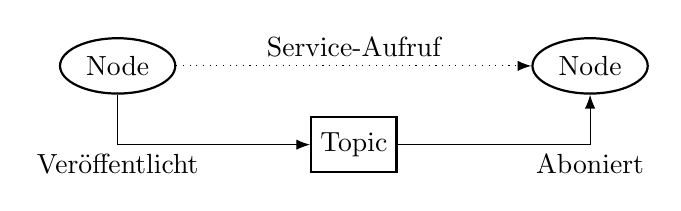
\begin{tikzpicture}[
        auto,
        defaultS/.style={
            thick,
            fill=white,
            align=center,
            minimum height=2em,
            draw=black
        },
        boxS/.style={
        	defaultS,
        	rectangle
        },
        ellipseS/.style={
        	defaultS,
        	ellipse
        },
        arrowS/.style={
            -{Latex[length=0.5em]}
        },
        lineS/.style={-},
    ]
    
	\node[ellipseS] (N1) at (0,1) {Node};
	\node[ellipseS] (N2) at (6,1) {Node};
	\node[boxS] (T) at (3,0) {Topic};
	
	\draw[arrowS] (N1) |- node[midway,below]{Veröffentlicht} (T);
	\draw[arrowS] (T) -| node [midway,below] {Aboniert} (N2);
	\draw[arrowS,dotted] (N1) -- node [midway,above] {Service-Aufruf} (N2);
    
    \end{tikzpicture}
    \caption{Einfacher ROS-Graph}
    \label{fig:ros-graph}
\end{figure}


%%%%%%%%%%%%%%%%%%%%%%%%%%%%%%%%%%%%%%%%%%%%%%%%%%%%%%%%%%%%%%%%%%%%%%%%%%%%%%%
\endinput
%%%%%%%%%%%%%%%%%%%%%%%%%%%%%%%%%%%%%%%%%%%%%%%%%%%%%%%%%%%%%%%%%%%%%%%%%%%%%%%


\subsubsection*{Nodes}

Eine Node ist ein Teilnehmer im \ac{ROS} Graphen, der über verschiedene Schnittstelle mit anderen Nodes kommuniziert. Dabei können sich die anderen Nodes im selben, in einem anderen Prozess oder auch auf einem anderen Rechner befinden. Nodes sind typischerweise die Recheneinheiten in einem ROS-Graphen, wobei jede Node eine logische Aufgabe erfüllt.

Nodes können Daten über sogenannte Topics veröffentlichen, um sie an andere Nodes zu senden. Andere Nodes können dann diese Topics abonieren, um Daten von dieser Node zu erhalten. Zusätzlilch können Nodes einen sogenannten Service-Server bereitstellen und für andere Nodes Berechnungen durchführen. Beliebig viele andere Nodes können bei diesem Service-Server Berechnungen in ihrem Namen durchführen lassen. Für länger dauernde Berechnungen können Nodes einen sogenannten Action-Server bereitstellen, der zusätzlich zum Service-Server die Möglichkeit bietet, Berechnungen Abzubrechen und fortlaufende Rückmeldungen über den Stand der Berechnungen zu liefern. Um das verhalten von Nodes während der Laufzeit zu beeinflussen, können diese konfigurierbare Parameter bereitstellen.

Oft stellen Nodes eine komplexe Kombination auws den oben beschriebenen Funktionalitäten da, indem sie zur gleichen Zeit mehrere Topics veröffentlichen und abonieren und verschiedene Services und Actions bereitstellen und von anderen Nodes verwenden.

Verbindungen zwischen Knoten werden automatisch durch die \ac{ROS} zugrundeliegende Middleware hergestellt.

\subsubsection*{Topics}

Topics sind einer der drei Arten von Schnittstellen, die \ac{ROS} bereitstellt und werden für kontinuierliche Datenströme wie Sensorinformationen oder Informationen über den Zustand des Roboters verwendet.

Topics funktionieren nach dem Publish-Subscribe-Prinzip \cite{baldoni2007}.
Hier gibt es zwei Gruppen von Beteiligten, eine die Daten produziert und sendet (Publisher) und eine welche diese empfängt und verarbeitet (Subscriber). Beide Gruppen Nutzen das Topic um miteinander in Kontakt zu treten. Dabei kann es in einem Topic keine oder beliebig viele Publisher geben und ebenso keine oder beliebig viele Subscriber.

\subsubsection*{Services}

Services in \ac{ROS} ermöglichen den Aufruf von Prozeduren in anderen Nodes. Anfragen werden durch eine Node initiiert und durch eine andere Node (den Service-Server) akzeptiert, welcher daraufhin eine Berechnung ausführt. Da die anfragende Node meißtens wartet, bis das Ergebnis eingetroffen ist, werden Services meistens für schnelle Berechnungen verwendet. Services bestehen aus einem Server an den beliebig viele Nodes Anfragen stellen können und werden wie Topics eindeutig durch einen Namen identifiziert. 

\subsubsection*{Actions}

Actions in \ac{ROS} fungieren ähnlich wie Services, sind jedoch auf lang laufende Prozeduren ausgelegt. Wie bei Services sendet eine Node eine Anfrage, hier jedoch an einen Action-Server. Anders als Services können Actions zusätzlich zum Ergebnis fortlaufende Rückmeldungen liefern und bieten die Möglichkeit zum Abbruch durch die anfragende Node. All dies führt jedoch zum einem Mehraufwand beim  erstellen der Verbindung.

\section{Verarbeitung von Audiosignalen}
Nachdem nun im letzten Kapitel Grundlagen über die Arbeit mit Robotern vermittelt wurde soll nun der Fokus auf der Audiosignalverarbeitung liegen. Da es sich hierbei nicht um eine Grundlagen Arbeit handelt wird grundsätzliches Wissen im Bereich Audiosignale und deren Eigenschaften vorausgesetzt. Dieses Kapitel soll einen Überblick darüber schaffen, welche Schritte notwendig sind, um eine Audiosignal erfolgreich zu analysieren und welche Methoden es grundsätzlich für diese Schritte gibt. Eine genauere Analyse der aktuell genutzten Methoden findet in Kapitel \ref{Kapitel3} statt. 

\subsection{Rauschen in Audiosignalen}
Rauschen bezeichnet in der Akustik und Signalverarbeitung jede Art von unerwünschtem Signal, das das Nutzsignal überlagert und dessen Qualität oder Verständlichkeit mindert. Als Maß von Rauschen in Audiosignalen gibt es das Signal-Rausch-Verhältnis (SNR, von englisch Signal-to-Noise Ratio). Es wird üblicherweise in Dezibel (dB) ausgedrückt und gibt an, wie viel höher das Niveau des gewünschten Signals im Vergleich zum Niveau des Rauschens ist. Ein höheres SNR bedeutet, dass das Signal im Verhältnis zum Rauschen stark ist, was allgemein mit einer besseren Qualität des Signals gleichgesetzt wird.


\subsubsection{Rauschquellen}
Nachfolgend sind mögliche Rauschquellen aufgeführt, welche in Audioaufnahmen von robotischen Schleifprozessen auftreten können. Wichtig an dieser Stelle ist zu bemerken, dass nicht alle hier aufgeführten Rauschquellen in diesem speziellen Anwendungsfall als ungewolltes Rauschen aufgefasst werden kann. Vielmehr muss bestimmtes Rauschen analysiert werden um die für diese Arbeit notwendigen Informationen zu beschaffen und eine spätere Klassifizierung vorzunehmen. Welche Rolle die einzelnen Rauschquellen spielen wird zu einem späteren Zeitpunkt bei der Umsetzung der tatsächlichen Rauschfilterung nochmals erläutert.

\begin{enumerate}
    \item \textbf{Mechanisches Rauschen}: Dieses Rauschen entsteht durch die Bewegung mechanischer Komponenten des Roboters und der Schleifausrüstung. Dazu gehören Vibrationen, die durch Unwuchten, Lagerfehler oder die Interaktion des Schleifwerkzeugs mit dem Werkstück entstehen. \cite{xiang2023}
    
    \item \textbf{Elektrisches Rauschen}: Elektrisches Rauschen kann aus der Roboterelektronik oder der Umgebung kommen. Dazu zählen Störungen durch elektromagnetische Felder, die von Motoren, Schaltern und anderen elektronischen Geräten erzeugt werden. \cite{xiang2023}
    
    \item \textbf{Akustisches Rauschen}: Umgebungsgeräusche, wie sie in industriellen Umgebungen üblich sind, können ebenfalls aufgezeichnet werden. Dazu zählen Gespräche, Geräusche anderer Maschinen und Werkzeuge sowie Lärm von Lüftungsanlagen. Zusätzlich können bei Schleifprozessen auch Windgeräusche entstehen, da das Schleifgerät auf eine sehr hohe Drehzahl beschleunigt wird und dadurch Luft umhergewirbelt wird. \cite{xiang2023}
    
    \item \textbf{Interferenzen durch Material und Werkzeug}: Die Art des bearbeiteten Materials und die Beschaffenheit des Schleifwerkzeugs können ebenfalls zu spezifischen Rauschmustern führen. Unterschiedliche Materialien und Werkzeuge erzeugen unterschiedliche Schwingungen und Geräuschpegel. \cite{plos2021}
    
    \item \textbf{Resonanzen im Aufnahmesystem}: Die Komponenten des Audioaufnahmesystems selbst (wie Mikrofone und ihre Befestigungen) können Resonanzen aufweisen, die das aufgezeichnete Signal verzerren. So können auch Resonanzen durch das Audiokabel auftreten, welches beim Schleifprozess Vibrationen ausgesetzt ist.
    
    \item \textbf{Digitales Rauschen}: Bei der Digitalisierung des Audiosignals kann digitales Rauschen auftreten, insbesondere wenn die Hardware nicht hochwertig ist oder falsch kalibriert wurde. Dies kann zu einem Verlust an Klangtreue und Präzision führen. \cite{plos2021}
    
\end{enumerate}

\subsubsection{Filtertechniken}
Da nun ein Überblick darüber geschaffen wurde, was Rauschen ist gilt es nun Möglichkeiten zu finden ungewolltes Rauschen aus der Audiospur zu entfernen. Eine Möglichkeit dies umzusetzen sind Filter.  Es folgt nun eine Übersicht über die gängigsten Filtertypen und ihre allgemeine Anwendung im Kontext der genannten Rauschquellen bei robotischen Schleifprozessen:

\begin{enumerate}

\item \textbf{Tiefpassfilter}
Ein Tiefpassfilter lässt Frequenzen unterhalb einer bestimmten Grenzfrequenz passieren und dämpft Frequenzen oberhalb dieser Grenze.

Anwendung:
\begin{itemize}
    \item Mechanisches Rauschen: Kann effektiv reduziert werden, wenn die Vibrationen zu hochfrequenten Geräuschen führen.
    \item Elektrisches Rauschen: Hochfrequentes Rauschen von elektronischen Komponenten kann gemindert werden.
\end{itemize}

\item \textbf{Hochpassfilter}
Ein Hochpassfilter lässt Frequenzen oberhalb einer bestimmten Grenzfrequenz passieren und dämpft niedrigere Frequenzen.

Anwendung:
\begin{itemize}
    \item Akustisches Rauschen: Tiefere Umgebungsgeräusche, wie das Brummen von Maschinen, können herausgefiltert werden.
\end{itemize}

\item \textbf{Bandpassfilter}
Ein Bandpassfilter lässt nur Frequenzen innerhalb eines bestimmten Bereichs passieren und dämpft Frequenzen außerhalb dieses Bereichs.

Anwendung:
\begin{itemize}
    \item Interferenzen durch Material und Werkzeug: Wenn das Rauschen oder die nützlichen Signale in einem bekannten Frequenzband liegen, kann ein Bandpassfilter eingesetzt werden.
\end{itemize}

\item \textbf{Bandstoppfilter (Notch-Filter)}
Ein Bandstoppfilter, auch als Notch-Filter bekannt, dämpft Frequenzen in einem schmalen Bereich und lässt Frequenzen außerhalb dieses Bereichs passieren.

Anwendung:
\begin{itemize}
    \item Resonanzen im Aufnahmesystem: Spezifische Resonanzfrequenzen, die durch die Aufnahmeausrüstung verursacht werden, können gezielt unterdrückt werden.
\end{itemize}
\end{enumerate}

\subsection{Fourier-Transformation}
Die Fourier-Transformation ist ein grundlegendes Werkzeug bei der Analyse von Audiosignalen. Sie ermöglicht ein Signal aus der Zeitdomäne in die Frequenzdomäne zu transformieren. Das heißt, das Signal wird in seine Frequenzen und die dazugehörigen Amplituden zerlegt. Benannt ist sie nach dem französischen Mathematiker Jean-Baptiste J. Fourier, der im 19. Jahrhundert die Herzfrequenz von Menschen untersuchte und dabei wichtige Grundlagen auf diesem Gebiet entwickelte \cite{Fourier1822}.

Im Wesentlichen zerlegt die Fourier-Transformation ein zeitabhängiges Signal in eine Summe von Sinus- und Kosinusfunktionen unterschiedlicher Frequenzen und Amplituden. 
Diese Bestandteile werden als Frequenzkomponenten des Signals bezeichnet. Das Ergebnis der Fourier-Transformation ist das Frequenzspektrum des ursprünglichen Signals, das angibt, welche Frequenzen im Signal enthalten sind und mit welcher Amplitude diese vertreten sind \cite{Wirsing2020}.

\begin{figure}[H]
    \centering
    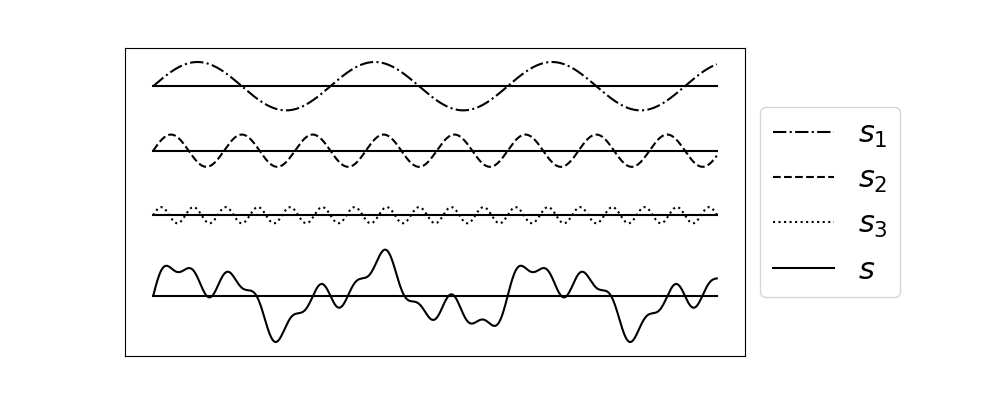
\includegraphics[width=1\linewidth]{images/simple_signal.png}
    \caption[Beispiel Signal \(s\)] {Ein Signal \(s\) zusammengesetzt aus verschiedenen Sinusfunktionen \\ \(s_1 : x \mapsto 1.5 \cdot sin(2x)\), \(s_2 : x \mapsto 1 \cdot sin(5x)\), \(s_3 : x \mapsto 0.5 \cdot sin(11x)\)}
    \label{fig:simple_signal}
\end{figure}

Beispielhaft betrachten wir das Signal \(s\) aus Abbildung \ref{fig:simple_signal}.
Dabei ist das Signal \(s\) die Summe folgender drei Sinusfunktionen:
\begin{align*}
s_1(x) =& 1.5 \cdot sin(2x) \\
s_2(x) =& 1 \cdot sin(5x) \\
s_3(x) =& 0.5 \cdot sin(11x) \\
\end{align*}
Die Sinusfunktionen haben jeweils, unterschiedliche Frequenzen und Amplituden:

\begin{itemize}
    \item \(s_1\) hat eine Frequenz von \(2\) und eine Amplitude von \(1.5\)
    \item \(s_2\) hat eine Frequenz von \(5\) und eine Amplitude von \(1\)
    \item \(s_3\) hat eine Frequenz von \(11\) und eine Amplitude von \(0.5\)
\end{itemize}

\begin{figure}[H]
    \centering
    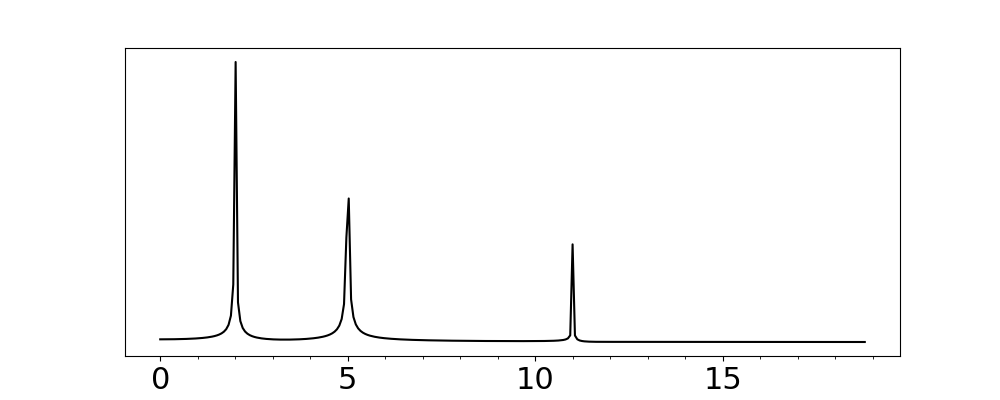
\includegraphics[width=1\linewidth]{images/simple_fft.png}
    \caption[Fourier-Transformation des Signals \(s\)] {Fourier-Transformation des Signals \(s\) aus Abbildung \ref{fig:simple_signal}}
    \label{fig:simple_fft}
\end{figure}

Abbildung \ref{fig:simple_fft} zeigt die Frequenzkomonenten des Signals \(s\) nach der Fourier-Transformation. Auf der x-Achse sind dabei die Frequenzen aufgetragen und auf der y-Achse die Amplituden dieser Frequenzen.
Man erkannt deutlich drei Peaks.
Einen Peak bei einer Frequenz von \(x_1 = 2\) mit einer relativ hohen Ausprägung, einen Peak bei \(x_2 = 5\) mit einer deutlich niedrigeren Ausprägung und einen bei \(x_3 = 11\) mit der niedrigsten Ausprägung.

\subsection{Wavelet} \label{ss:wavelet}

Ein Wavelet ist eine mathematische Funktion, die, wie die oben genannte Fourier-Transformation zur Analyse von Signalen verwendet werden kann. Ein Problem bei der Fourier-Transformation ist jedoch, das die Information über die Zeit verloren geht. So besitzen zum Beispiel ein Audiosignal und dessen Spiegelung exakt das gleiche Frequenzspektrum. \cite{Lee1999}

Im Gegensatz dazu kann man mithilfe einer, Wavelet-Transformation das Signal sowohl in die Zeit- als auch in dessen Frequenzdomänen zerlegen. Dies bedeutet, dass Wavelets Informationen über die Frequenzverteilung eines Signals sowie über die zeitliche Lokalisierung von Ereignissen liefern können.

\begin{figure}[H]
    \centering
    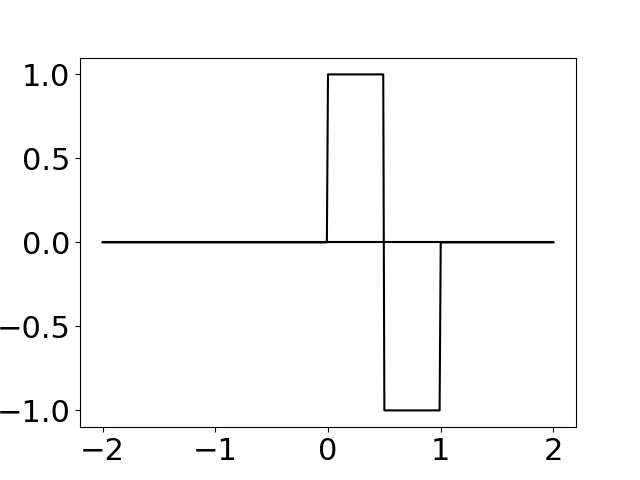
\includegraphics[width=0.5\linewidth]{images/haar.png}
    \caption{Haar-Wavelet}
    \label{fig:haar-wavelet}
\end{figure}

Das Besondere an Wavelets ist, dass sie lokalisiert sind, was bedeutet, dass sie nur in einem begrenzten Bereich des Signals signifikant von null abweichen, im Gegensatz zu den sinusförmigen Funktionen der Fourier-Transformation, die über das gesamte Signal ausgedehnt sind. Dies macht Wavelets besonders nützlich für die Analyse von Signalen mit diskreten Ereignissen oder abrupten Veränderungen, wie zum Beispiel bei der Analyse periodischen Wetterphänomenen \cite{Schulte2019}.

\begin{figure}[H]
    \centering
    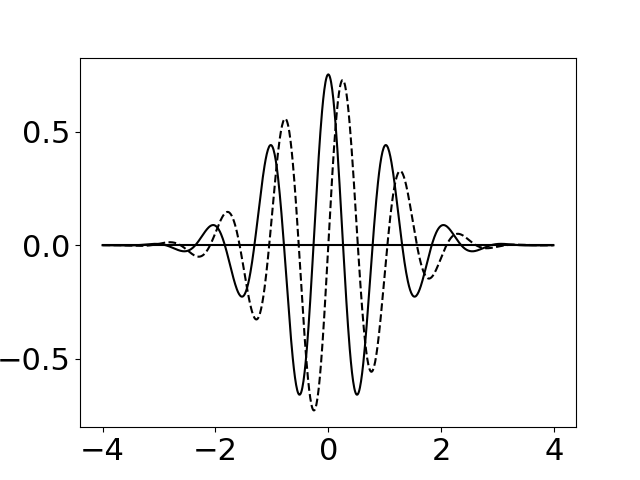
\includegraphics[width=0.5\linewidth]{images/morlet.png}
    \caption{Morlet-Wavelet}
    \label{fig:morlet-wavelet}
\end{figure}

Eine häufig verwendete Wavelet-Funktion ist das Haar-Wavelet (siehe Abbildung \ref{fig:haar-wavelet}):

\begin{equation} \label{eq:haar}
    \psi (t) \; = \; 
    \begin{cases}
        1 \quad &0 \leq \: t \: < \: {1 \over 2} \\
        -1      &{1 \over 2}  \leq \: t \: < \: 1 \\
        0       &\texttt{sonst}
    \end{cases}
\end{equation}

Es ist die einfachste Form des Wavelets. Ein weiteres, häufig verwendetes Wavelet ist das Morlet-Wavelet (siehe Abbildung \ref{fig:morlet-wavelet}):

\begin{equation} \label{eq:morlet}
    \psi (t) \; = \; \pi^{-{1 \over 4}} e^{i\omega_0 t}e^{-{t^2 \, / 2}}
\end{equation}

Wobei \(\omega_0\) (hier \(\omega_0 \; = \; 6\)) die Anzahl der Maxima im Wavelet verändert. \cite{Torrence1998}

%%%%%%%%%%%%%%%%%%%%%%%%%%%%%%%%%%%%%%%%%%%%%%%%%%%%%%%%%%%%%%%%%%%%%%%%%%%%%%%
\endinput
%%%%%%%%%%%%%%%%%%%%%%%%%%%%%%%%%%%%%%%%%%%%%%%%%%%%%%%%%%%%%%%%%%%%%%%%%%%%%%%

\chapter{Stand der Dinge}
\label{Kapitel3}

Das vorliegende Kapitel widmet sich der Untersuchung des aktuellen Forschungsstands auf dem Gebiet der akustischen Vermessung von robotischen Schleifprozessen zur prädiktiven Wartung. Anschließend wird auf die spezifischen Herausforderungen und Möglichkeiten eingegangen, die die akustische Vermessung in robotergestützten Schleifanwendungen bietet.
    

\section{Analyse des Audiosignals}
%https://www.intechopen.com/chapters/74096

Wie bereits im Kapitel \ref{Kapitel2} vermittelt, werden Informationen aus Audiosignalen extrahiert, indem das vorliegende Audiosignal in den Frequenzbereich umgewandelt wird. Dafür werden die Methoden der Fourier-Transformation und der Wavelet-Transformation genauer betrachtet. Im Folgenden werden nun praktische Umsetzungen zu diesen Methoden aufgezeigt.

\subsection{Fast Fourier transform}

Angefangen bei der praktischen Umsetzung der Fourier-Transformation. Hierzu hat im Laufe der Zeit festgestellt, dass der ursprüngliche Algorithmus sehr komplex und zeitaufwendig ist und somit bei der praktischen Anwendung nicht effektiv eingesetzt werden kann. Aus diesem Grund haben sich zahlreiche Heuristiken Entwickelt, welche diese Berechnung schneller machen und dennoch gute Ergebnisse erzielen. Diese Heuristiken sind heutzutage allgemein als \ac{FFT} bekannt. \cite[155f.]{Meyer2000} Praktisch gesehen ist fast jede praktische Implementierung der \ac{FT} eigentlich eine \ac{FFT}. \cite[6]{Heckbert1995}

\paragraph{Cooley und Tukey}
   
Der \ac{FFT}-Algorithmus von Cooley und Tukey, oder auch Radix-2-Algorithmus genannt, ist der bekannteste Algorithmus für die schnelle Berechnung einer \ac{FT}, da er sowohl leicht zu implementieren ist, als auch konsistent sehr gute Ergebnisse liefert. \cite[156ff.]{Meyer2000} 
Dies erreicht der Algorithmus, indem er die \ac{DFT} direkt und nicht über Matrixmultiplikation berechnet. Der Trick dahinter ist die Nutzung von Rekursion. So wird die zu berechnende Matrix wieder und wieder in zwei Teile aufgeteilt, bis die Teile so klein sind, dass die Anwendung der \ac{DFT} nur geringfügig komplex ist. Die einzige Bedingung hierfür ist, dass die Anzahl der Objekte eine Zweierpotenz sein muss. \cite{Rabiner1969} Erreichbar ist dies aber mit einfachen 0-padding. \cite[41 ff.]{Aamir2005} Diese Implementierung alleine ist schon eine gültige \ac{FFT}, jedoch fehlt hierbei ein weiterer Trick, welcher den Algorithmus besonders macht. Dieser Trick sind sogenannte Butterfly-Diagramme. Diese Diagramme überwachen und sortieren die Elemente in jedem Zustand der \ac{FFT}. Sie sorgen dafür, dass die Listen, auf welchem die \ac{DFT} durchgeführt wird, Werte enthalten die nahe beieinander liegen, wodurch die Berechnung der DFT schneller durchgeführt werden kann. \cite[3ff.]{Burrus2009} \cite[7]{Heckbert1995} Dafür werden immer Approximationen von zwei Werte verglichen, weshalb der Algorithmus auch Radix-2-Algorithmus genannt wird.  Diese Sortierung reduziert am Ende die Komplexität mehr als sie selbst bei der Implementierung erzeugt, wodurch der Algorithmus effizienter wird. Auf die dahinter steckenden mathematischen Beweise wird in dieser Arbeit nicht weiter eingegangen.  Bei Interesse werden weiterführende Quellen empfohlen.  \cite[9f.]{Heckbert1995} \cite{Bekele2016}

Neben dem Algorithmus von Cooley und Tukey gibt es noch weitere Algorithmen, welche die \ac{DFT} durch Heuristiken weniger komplex berechnen. Die bekanntesten Vertreter hierbei sind Primfaktor-Algorithmen und die Chirp-z-Transformation. Im Allgemeinen zielen die Primfaktor-Algorithmen darauf ab die Anzahl an Multiplikationen während einer \ac{DFT} zu reduzieren, indem die Anzahl an Additionen erhöht wird. Da Additionen weniger komplexe mathematische Operationen sind, sinkt somit die Komplexität zur Berechnung der \ac{DFT}. \cite{Temperton1992} Die Chirp-z-Transformation oder auch Bluestein-FFT genannt, berechnet die \ac{DFT}, indem diese als komplexe Faltung betrachtet wird, welche stattdessen gelöst wird. Dadurch wird die Einschränkung, dass die Anzahl der Daten eine Zweierpotenz sein muss aufgehoben. \cite{Rabiner1969} Auf eine genauere Erläuterung dieser Alternativen und der mathematischen Grundlagen dahinter, wird in dieser Arbeit verzichtet, da wie an späterer Stelle genauer erläutert die für die Umsetzung genutzten Implementierungen auf dem Algorithmus von Cooley und Tukey beruhen.

\subsection{Kurzzeit-Fourier Transformation}
    
Wie bereits im Kapitel Grundlagen \ref{Kapitel2} erläutert ist einer der größten Nachteile der \ac{FT}, dass jegliche Informationen über die Zeit verloren geht. In Falle der Schleifanalyse bedeutet dies, dass nach der Anwendung der \ac{FT} auf eine Audiospur nicht erkennbar ist, wann in dieser Audiospur beispielsweise eine Anomalie auftritt, des Weiteren kann es auch passieren, dass die auftretende Anomalie in einem so kurzen Zeitabschnitt geschieht, sodass diese im letztendlichen Ergebnis des \ac{FT} völlig untergeht. Die einfachste Lösung hierzu ist, dass man die \ac{FT} nicht auf das ganze Audiosignal anwendet, sondern immer nur auf einen kleinen Teil. Dieser Algorithmus wird dann als \ac{STFT} bezeichnet, wobei die Umsetzung der \ac{FT} immer durch eine im letzten Kapitel \ref{Kapitel2} erläuterte \ac{FFT} stattfindet. \cite{Okumura2011}

\paragraph{Funktionsweise der Kurzzeit-Fourier-Transformation}
    
Grundsätzlich gesprochen funktioniert die \ac{STFT}, indem ein Teil-Zeitabschnitt festgelegt wird, auf welchem dann eine \ac{STFT} angewendet wird. Der Zeitabschnitt wird dann verschoben, dieses Vorgehen wird dann rekursiv weitergeführt, bis das ganze Audiosignal betarchtet wurde. Im Beispiel gesprochen heißt das, dass bei einem 10-sekündigen Audiosignal eine \ac{FFT} immer aus z.B. eine Sekunde angewendet wird. Die Ergebnisse dieser 10 \ac{FFT} werden anschließend zusammengefasst. \cite[69]{Kiencke2008}
Dieses Schrittweise ablaufen des Signals kann schon als \ac{STFT} betarchtet werden, jedoch gibt es viele Parameter, welche die \ac{STFT} beeinflussen können, um so das Ergebnis zu optimieren. So entstanden die Idee eines Fensters und des Versatzes. \cite[5f.]{Okumura2011} Ein Fenster besitzt hierbei eine feste Breite, welche dann auf den Zeitabschnitt des Signals gelegt werden kann, auf welchen eine \ac{FFT} durchgeführt werden soll. Die Wahl der Breite bestimmt die Genauigkeit des Ergebnisses, welche sich in Zeitgenauigkeit und Frequenzgenauigkeit aufteilen lässt. \cite{jacobsen2003} Diese Genauigkeiten können nie gleichzeitig hoch sein, dieses Problem ist in der Quantenmechanik auch als ,,Uncertainty Principle'' bekannt. \cite{uncertainty2024} Will man nun die Zeitgenauigkeit erhöhen, so  muss die Fenster-Größe verringert werden. Im Gegenzug sinkt jedoch die die Frequenzgenauigkeit. 
    
Der zweite Parameter einer \ac{STFT} ist der Versatz, dieser beschreibt wie weit das Fenster sich nach jeder Anwendung der \ac{FFT} verschiebt. Der Versatz wird typischerweise nun kleiner als das Fenster gewählt, sodass jeder Datenpunkt nicht nur einmal sondern mehrmals ausgewertet wird. Dieses mehrfache Auswerten jedes Datenpunktes erhöht zum einen die Genauigkeit des Ergebnisses und glättet zum anderen den Übergang zwischen den Ergebnissen zweier nachfolgender \ac{FFT}. Je kleiner der Versatz, desto höher ist jedoch auch der Berechnungsaufwand. \cite{jacobsen2003} Die Abbildung \ref{fig:hop-overlpa-fenster} zeigt die Anwendung solcher Fenster und des Versatzes im allgemeinen und die Abbildung \ref{fig:different-overlaps} zeigt die Auswirkung verschiedener Versetze auf ein Ergebnis.
    
    \begin{figure}[H]
        \centering
        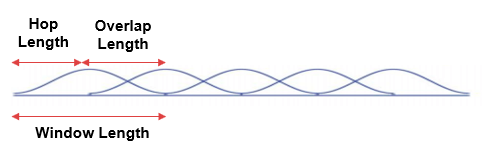
\includegraphics[width=0.5\linewidth]{images/hop-overlpa-fenster.png}
        \caption{Visualisierung des Fensters und des Versatzes \cite{hopAWindow}}
        \label{fig:hop-overlpa-fenster}
    \end{figure}
    
    \begin{figure}[H]
        \centering
        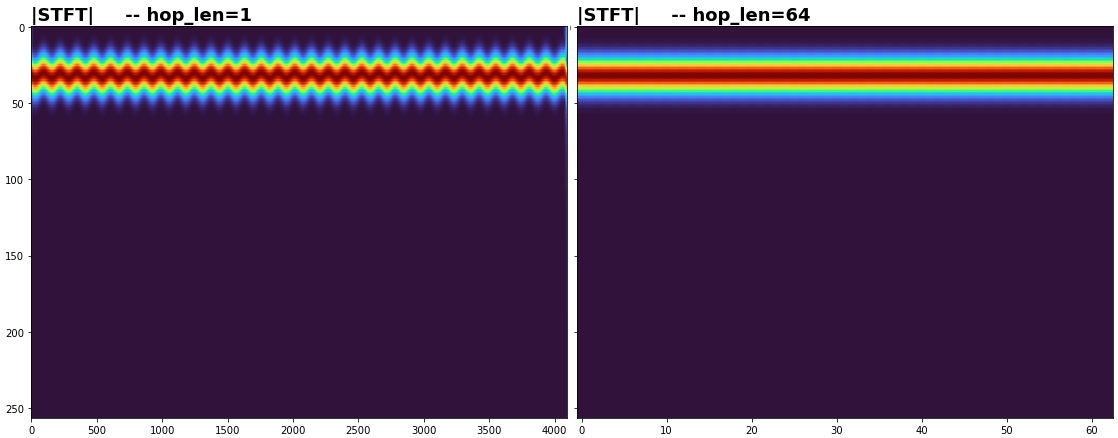
\includegraphics[width=0.5\linewidth]{images/different-overlaps.png}
        \caption{Auswirkungen verschiedener Versätze \cite{versätze}}
        \label{fig:different-overlaps}
    \end{figure}
    %https://dsp.stackexchange.com/questions/19311/stft-why-overlapping-the-window
    
Zusätzlich zu der Wahl des Versatzes lässt sich aber auch das Fenster anpassen. So kann das Fenster nicht nur eine Breite haben, sondern es kann zusätzlich eine Funktion gewählt werden, die die Daten innerhalb des Fensters manipuliert. Die einfachste Funktion spiegelt die zu analysierenden Daten 1zu1 wieder. Jedoch ist es auch möglich beispielsweise eine Funktion als Grundlage zu benutzen, welche die Daten, welche im Zentrum des Fensters liegen stärker gewichtet. Die Abbildungen \ref{fig:Veranschaulichung verschiedener Fenster und deren Frequenzspektren} zeigen verschiedene Beispiele solcher Fenster. 

    \begin{figure}[H]
        \centering
        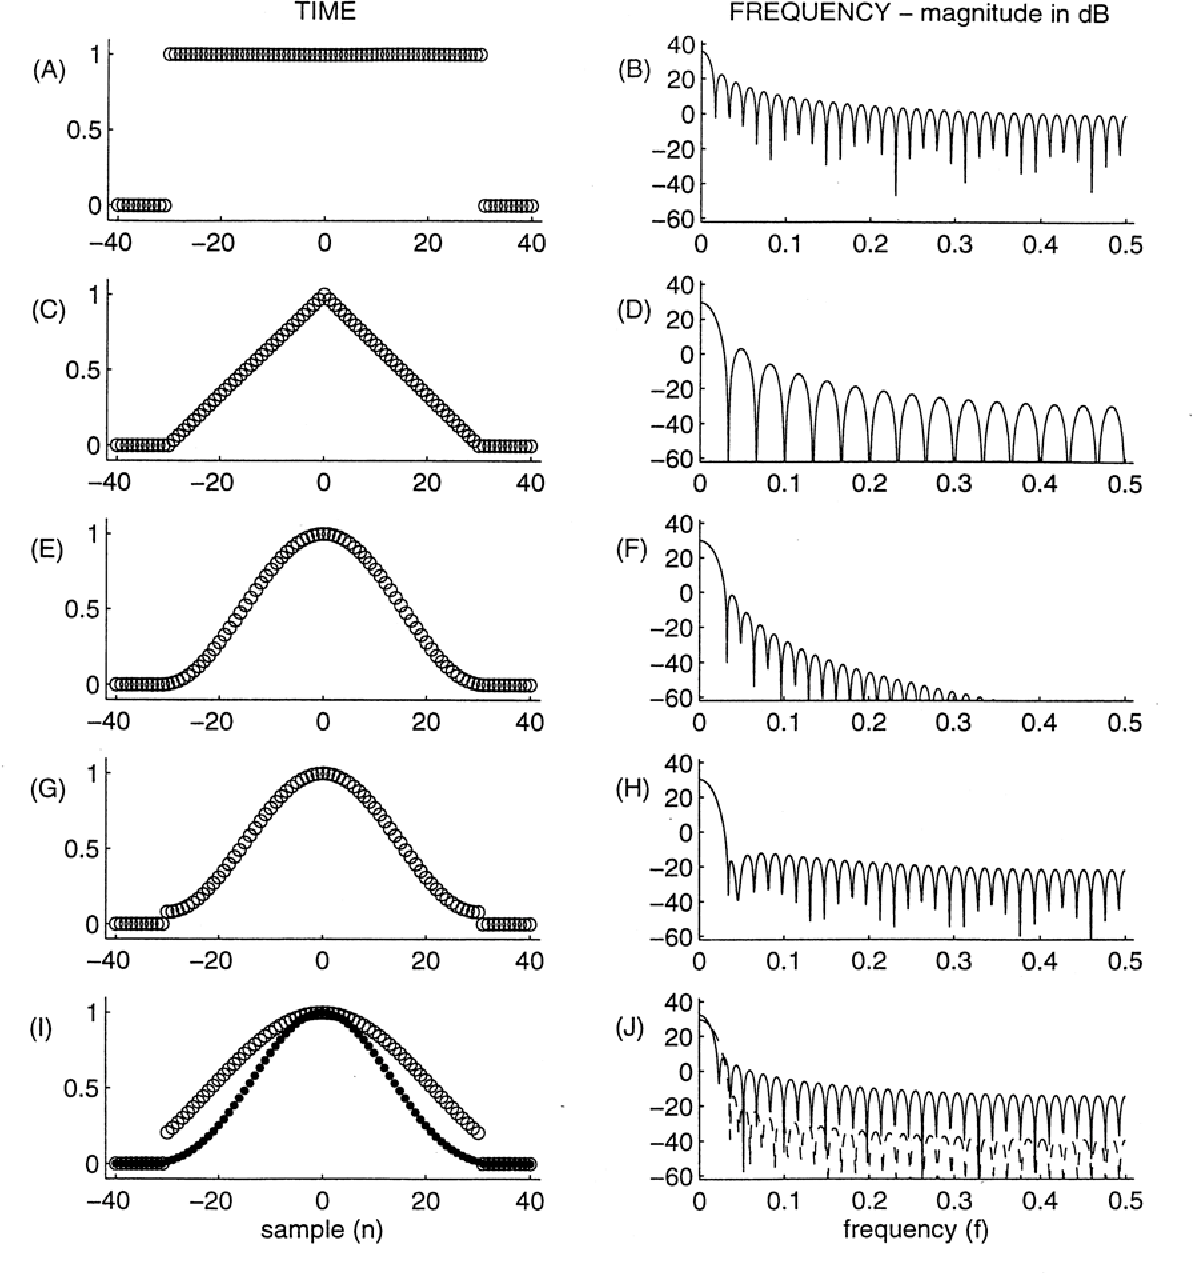
\includegraphics[width=0.5\linewidth]{images/Veranschaulichung verschiedener Fenster und deren Frequenzspektren.png}
        \caption{Veranschaulichung verschiedener Fenster und deren Frequenzspektren} \cite{windowFunctions}
        \label{fig:Veranschaulichung verschiedener Fenster und deren Frequenzspektren}
    \end{figure}
    
Der Vorteil der durch den in Abbildungen \ref{fig:Veranschaulichung verschiedener Fenster und deren Frequenzspektren} gezeigten Fenster entstehen dadurch, dass wie bereits zuvor erwähnt die am Rand des Fenster liegenden Datenpunkte durch die Wahl des Versatzes sowieso mehrfach analysiert werden und somit eine höhere Gewichtung im Endergebnis erhalten. Durch die stärkere Gewichtung der Zentralen Daten wird dem entgegengewirkt. Aus diesem Grund hat sich die Gaussian-Verteilung als gute Allgemeine Lösung etabliert, welche durch die Wahl der Standardabweichung auf den jeweiligen Versatz und zu lösendes Problem angewendet werden kann.
    
Zusammengefasst lässt sich festhalten, dass die Wahl der einzelnen Parameter stark von dem zu lösenden Problem abhängen. Durch die Notwendigkeit der Festlegung dieser Parameter entsteht auch das Problem, dass je nach Signalart oder Signallänge verschiedene Parameter zu verschiedenen Ergebnissen führen kann und die Wahl dieser Parameter somit einer hohen Komplexität unterliegen. So können die Parameter, welche gute Ergebnisse für ein Problem bei langen Signalen erzeugen schlechte Ergebnisse beim selben Problem und kurzen Signalen erzeugen. Kurz gesagt kann es sich als sehr schwierig herausstellen eine \ac{STFT} zu generalisieren, sei es auch nur für einen spezifischeren Anwendungsfall, wie die Analyse von Schleifgeräuschen. Inwiefern dieses Problem in diesem Fall besteht wird in der späteren Durchführung genauer erläutert, wenn tatsächlich mehrere verschiedene \ac{STFT} implementiert und ausgewertet werden.

\subsection{Kontinuierliche Wavelet-Transformation}

Die \ac{CWT} ist wie die \ac{STFT} eine Methode zur Analyse von Signalen. Wie bereits in \ref{ss:wavelet} beschrieben, bietet die \ac{WT} im Vergleich zur \ac{FT} den Vorteil, die zeitlichen Komponente der Signalen zu bewahren. 
Sie kommt an verschiedensten Bereichen zum Einsatz, wie zum Beispiel in der Meteorologie bei der Analyse von zyklischen Wetterphänomenen \cite{Torrence1999}.

\paragraph{Funktionsweise der Kontinuierlichen Wavelet-Transformation}

Bei der \ac{CWT} wird ein Signal mit einer skalierten und verschobenen Version eines sogenannten ,,Mother-Wavelet'' gefaltet. Beispiele für häufig verwendete Wavelets sind das in \ref{ss:wavelet} gezeigten Haar-Wavelet (siehe Abbildung \ref{fig:haar-wavelet}) welches durch Gleichung \ref{eq:haar} beschrieben wird und das Morlet-Wavelet (siehe Abbildung \ref{fig:morlet-wavelet}) welches durch \ref{eq:morlet} beschrieben wird. Die Transformation wird durch folgende Gleichung beschreiben \cite[92]{Schulte2019}:

\begin{equation}
W(a, b) = \int_{-\infty}^\infty x(t) \Psi^* \left( \frac{t - b}{a} \right) dt
\end{equation}

Hierbei stellt \(x(t)\) das zu analysierende Signal da und \(\Psi(t)\) das ,,Mother''-Wavelet. Mithilfe von \(a\) kann das Wavelet skaliert werden und mit \(b\) verschoben werden. 
Der Skalierungsparameter \(a\) variiert die Breite des Wavelets. Ein großer Skalar \(a\) entspricht dabei einer breiten Wavelet-Funktion und ermöglicht das Abtasten auf niedrigere Frequenzen. Dabei sinkt jedoch die Auflösung in der Zeit-Domäne. \cite{Torrence1998}

Der Parameter \(b\) gibt an, zu welchem Zeitpunkt die Analyse durchgeführt wird. Durch kontinuierliche Verschiebung des Wavelets entlang der Zeitachse kann die zeitliche Entwicklung einzelner Frequenzkomponenten des Signals verfolgt werden.

\paragraph{Beispielhafte Verwendung}

Um die Funktionsweise der \ac{CWT} zu veranschaulichen, betrachten wir zwei Beispiele, die anhand der folgenden Abbildungen dargestellt werden.

 \begin{figure}[H]
     \centering
            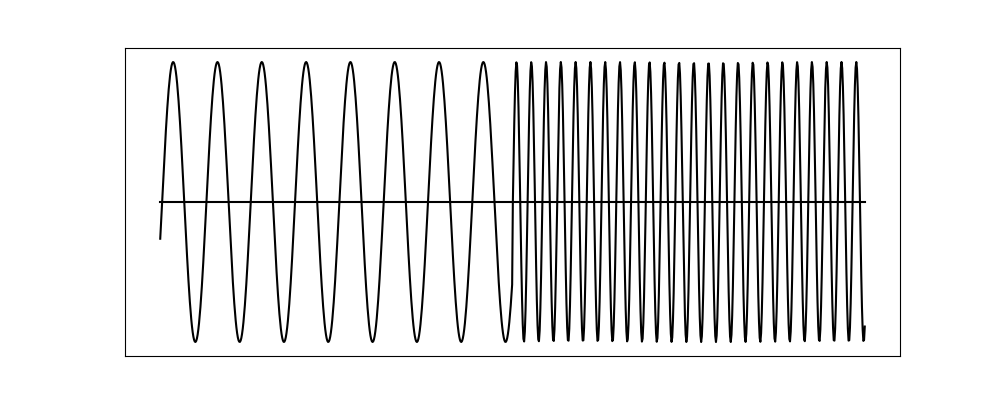
\includegraphics[width=0.9\linewidth]{images/aprupt_change_signal.png}
            \caption{Signal mit einer abrupter Frequenzänderung in der Mitte}
            \label{fig:aprupt_change_signal}
            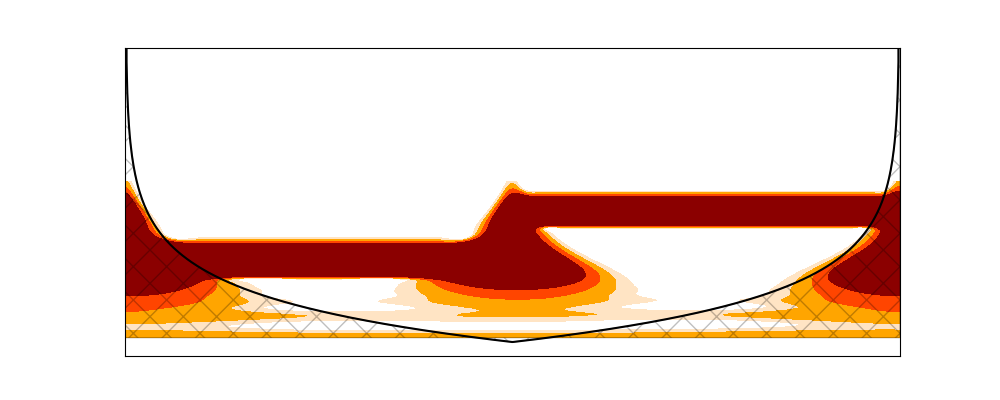
\includegraphics[width=0.9\linewidth]{images/aprupt_change_cwt.png}
            \caption[CWT Analyse eines Signals mit abrupter Frequenzänderung]{CWT Analyse des Signals von Abbildung \ref{fig:aprupt_change_signal}. Die Skalierung der y-Achse ist logarithmisch. Der schraffierte Bereiche stellen den so genannte ,,cone of influence'' da, in dem Randeffekte zu großen Einfluss haben} 
            \label{fig:aprupt_change_cwt}
        % \caption{Two pictures}
\end{figure}

Abbildung \ref{fig:aprupt_change_signal} zeigt ein Signal, das in der Mitte eine abrupte Frequenzänderung aufweist. Die zugehörige \ac{CWT}-Analyse ist in Abbildung \ref{fig:aprupt_change_cwt} dargestellt. Hier ist deutlich zu erkennen, dass die \ac{CWT} die zeitliche Position der Frequenzänderung erfasst. In der linken Hälfte der Analyse ist eine niedrige Frequenz dominant, während in der rechten Hälfte eine höhere Frequenz auftritt. Dies verdeutlicht die Fähigkeit der \ac{CWT}, sowohl zeitliche als auch frequenzielle Informationen des Signals präzise darzustellen.

\begin{figure}[H]   
     \centering
    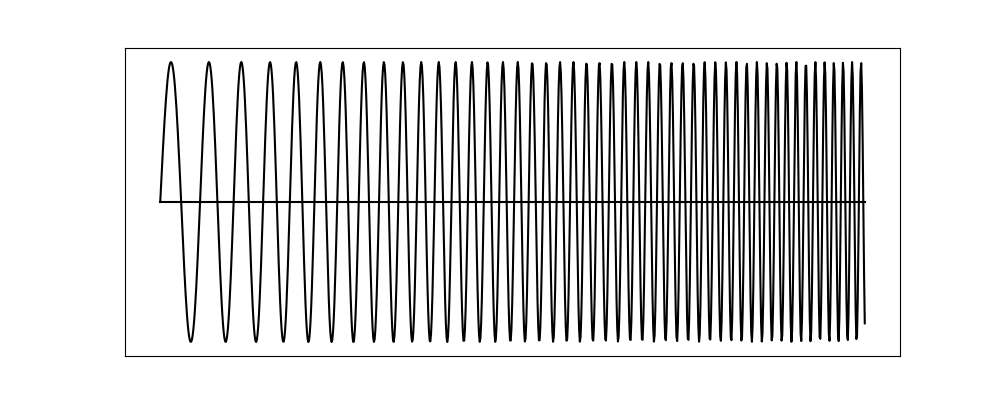
\includegraphics[width=0.9\linewidth]{images/continous_change_signal.png}
    \caption{Signal mit kontinuierlicher Frequenzänderung}
    \label{fig:continous_change_signal}   
    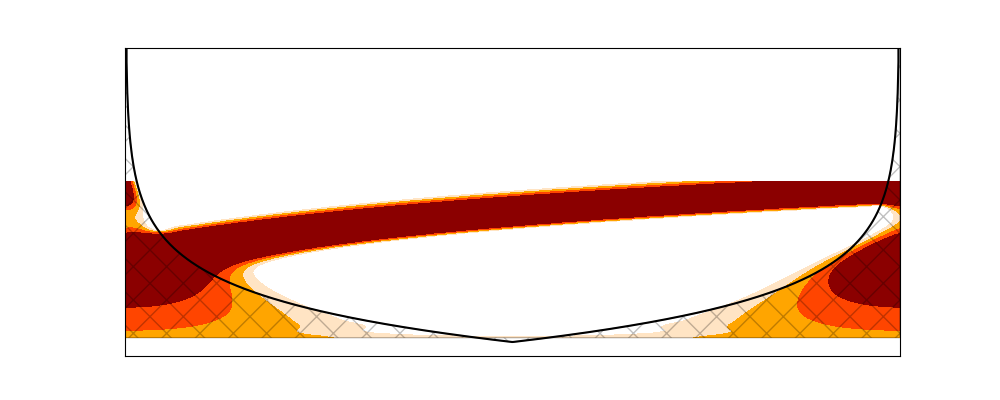
\includegraphics[width=0.9\linewidth]{images/continous_change_cwt.png}
    \caption[CWT Analyse eines Signals mit kontinuierlicher Frequenzänderung]{CWT Analyse des Signals von Abbildung \ref{fig:continous_change_signal}. Die Skalierung y-Achse ist logarithmisch. (Schraffierter Bereich siehe \ref{fig:aprupt_change_cwt})}
    \label{fig:continous_change_cwt}
% \caption{Two pictures}
\end{figure}

In Abbildung \ref{fig:continous_change_signal} sehen wir ein Signal mit einer kontinuierlichen Frequenzänderung. Die zugehörige \ac{CWT}-Analyse ist in Abbildung \ref{fig:continous_change_cwt} dargestellt. Hier zeigt die \ac{CWT}-Analyse eine kontinuierliche Änderung der Frequenz über die Zeit hinweg. Dies wird durch eine schrittweise Verschiebung des Frequenzbereichs in der Zeit-Frequenz-Darstellung deutlich. Diese Analyse ermöglicht es, den Verlauf der Frequenzänderungen im Signal über die Zeit präzise zu verfolgen.

Wie in den beiden Beispielen verdeutlicht wurde, bietet die \ac{CWT} Änderungen verschiedenster Art in Signalen identifizieren zu können. Somit bietet die \ac{CWT} ein vielseitiges Werkzeug, um zeitabhängige Besonderheiten in Signalen identifizieren und im Anschluss analysieren zu können.

\subsection{Signifikanztests}

Ein Problem, dass sich bei der Analyse mit Wavelets ergibt, ist das finden von signifikanten Ereignissen in der Zeit-Frequenz-Domäne, wie auch schon Lau in \cite[2401]{Lau1995} anmerkt. 

Dabei kann zwischen vier verschiedenen statistischen Signifikanztests unterschieden werden \cite{Schulte2019}:

\begin{enumerate}
    \item Point-wise tests
    \item Area-wise test
    \item Geometric test
    \item Cumulativ-area-wise tests
\end{enumerate}

Wir wollen im folgenden nur auf Point-wise und Area-wise tests eingehen.

\paragraph{Point-wise signifikance tests}
Bei Point-wise tests wird zuerst ein Signifikanzniveau ermittelt. Im Anschluss wird dann jeder Punkt mit diesem Signifikanzniveau verglichen um so konkrete Ereignisse zu erkennen.

Um Signifikanzniveaus für ein Waveletspektrum zu bestimmen, muss zunächst ein geeignetes Hintergrundspektrum gewählt werden, oft weißes Rauschen, mit gleichbleibender Leistung für alle Frequenzen. Ein weiteres häufig verwendetes Rauschen ist rotes Rauschen, bei dem die Leistung mit abnehmender Frequenz zunimmt. Diese Spektren dienen als Nullhypothese, gegen die das tatsächliche Spektrum verglichen wird. \cite[67f]{Torrence1998}

Wenn ein Peak im Waveletspektrum signifikant über dem Hintergrundniveau liegt, wird er als echtes Merkmal angenommen. So ist es möglich, Unterschiede zwischen wichtigen Ereignissen im Signal und zufälligen Schwankungen zu erkennen und Bereiche hoher statistischer Signifikanz zu identifizieren.

Wie Maraun und Kurths in \cite[511]{Maraun2004} hinweisen, haben Point-wise tests jedoch einige Nachteile:
So sind, um korrekte Signifikanzniveaus zu wählen oft Monte-Carlo Simulationen notwendig und es kann zu irreführenden Peaks kommen, welche die Auswertung verfälschen.

\paragraph{Area-wise signifikance-tests}

Area-wise signifikance-tests sind eine Erweiterung der Point-wise tests. Hierbei werden, wie beim Point-wise testing, alle Punkte mit einem zuvor ermittelten Signifikanzniveau verglichen. Zusätzlich dazu wird jedoch die Fläche der so entstandenen Flecken betrachtet \cite{Maraun2007}. Hierbei sind Flecken mit größerer Fläche statistisch signifikanter. Zusätzlich müssen diese Flecken eine gewisse Mindestgröße aufweisen, was dabei hilft, kleine, Falsch-Positive Flecken herauszufiltern. Dies hat jedoch zur Folge, das Area-wise signifikance-tests weniger sensitiv für kleine Ereignisse sind \cite{Schulte2016}. 

\section{Klassifizierung}

In folgenden Kapitel werden aktuelle Forschungen und wissenschaftliche Berichte im Bereich Klassifizierung mit KI vorgestellt. Diese Methoden sind vor allem wichtig, um zu sehen was bisher möglich ist. Eine KI Klassifizierung findet jedoch im Zuge der Arbeit nicht statt, vielmehr dient dieses Kapitel dazu, Klarheit darüber zu schaffen, wie es mit der Arbeit weiter gehen könnte. Dennoch ist es uns wichtig dieses Thema hier nicht zu kurz kommen zu lasse, da KI in vielen Bereichen immer mehr an Bedeutung gewinnt. Da wie in Kapitel \ref{Kapitel1} diese Arbeit eine Grundlage für weitere Arbeiten schaffen soll wird das Thema KI unabdingbar sein. 

\subsection{Verwendung von KI}
Die fortgeschrittene Analyse und Überwachung von Schleifprozessen mittels akustischer Daten stellt einen signifikanten Fortschritt in der Fertigungstechnologie dar, insbesondere durch die Anwendung von maschinellem Lernen und speziell tiefen neuronalen Netzwerken. Die Fähigkeit, aus dem kontinuierlichen Strom von Maschinengeräuschen präzise und nützliche Informationen zu extrahieren, hat weitreichende Implikationen für die Effizienz und Zuverlässigkeit industrieller Fertigungsprozesse. Maschinelles Lernen, insbesondere durch den Einsatz von Convolutional Neural Networks (CNNs), bietet eine effektive Lösung für die automatisierte Erkennung und Klassifizierung von Zustandsmerkmalen der Maschine basierend auf akustischen Signalen.

Neuronale Netzwerke sind besonders wertvoll in dieser Anwendung, da sie fähig sind, aus großen Datenmengen von Audiosignalen Muster zu erkennen und zu lernen, die für das menschliche Ohr nicht offensichtlich sind. Diese Fähigkeit, tiefergehende Einsichten aus den Audiodaten zu gewinnen, ohne auf vordefinierte Heuristiken oder manuell codierte Merkmale angewiesen zu sein, stellt einen Paradigmenwechsel dar. Durch Training mit umfangreichen Datensätzen können diese Modelle lernen, subtile akustische Unterschiede zu identifizieren, die auf spezifische Schleifzustände hinweisen. Dies verbessert nicht nur die Präzision in der Überwachung, sondern auch die Reaktionsfähigkeit des Produktionsprozesses, indem Anpassungen in Echtzeit ermöglicht werden, um optimale Betriebsbedingungen zu gewährleisten.


\subsection{Forschungsbeispiele und ihre Bedeutung}

In ihrer bahnbrechenden Studie \cite{Yang2019} untersuchten Yang und Rai die Anwendung von Convolutional Neural Networks (CNNs) zur akustischen Diagnostik von Maschinen mittels ,,Machine Auscultation'', analog zur medizinischen Auskultation, bei der Geräusche von Organen zur Diagnose genutzt werden. Ihre Forschung zielte darauf ab, abnormale Geräusche und Schwingungen, die während des Schleifprozesses auftreten, zu identifizieren und zu klassifizieren, speziell das Phänomen des Chatterns.

Das Team setzte CNNs ein, um die komplexen akustischen Signale, die von CNC-Maschinen während des Betriebs erzeugt werden, zu analysieren. Die Herausforderung bestand darin, aus den hochdimensionalen und oft verrauschten Daten nutzbare Informationen zu extrahieren. Die Forscher entwickelten ein System, das in der Lage war, aus den akustischen Daten zu lernen und diese zu verarbeiten, wodurch eine Echtzeit-Überwachung und -Analyse des Maschinenzustands ermöglicht wurde.

Die Ergebnisse von Yang und Rai zeigten, dass ihre CNN-basierten Modelle eine deutlich höhere Genauigkeit bei der Erkennung von Maschinenanomalien erreichen konnten als traditionelle Methoden. Besonders hervorzuheben ist die Fähigkeit des Modells, Chattern zu erkennen und zu klassifizieren, was zu einer signifikanten Verbesserung der Produktqualität und einer Reduzierung von Ausfallzeiten führen kann. Die Genauigkeit und Effizienz ihres Ansatzes wurde durch umfangreiche Tests und Validierungen bestätigt, wobei die Modelle eine bemerkenswerte Fähigkeit zur Unterscheidung zwischen normalen und abnormalen Betriebszuständen zeigten.

Die Studie von Cheng et al. \cite{Cheng2018} fokussierte sich auf die innovative Anwendung von Deep Convolutional Neural Networks (DCNNs) zur Zustandsüberwachung von Schleifbändern mittels akustischer Daten, die während des Schleifprozesses gesammelt wurden. Diese Forschungsarbeit verdeutlicht, wie DCNNs erfolgreich eingesetzt werden können, um den Verschleißzustand von Schleifwerkzeugen zu analysieren und vorherzusagen.

Cheng et al. entwickelten ein Modell, das darauf trainiert wurde, spezifische akustische Signaturen zu erkennen, die mit verschiedenen Verschleißgraden der Schleifbänder korrelieren. Durch das Training des Netzwerks mit einer umfangreichen Sammlung von Schleifgeräuschen konnten die Forscher eine hohe Genauigkeit in der Vorhersage des Werkzeugzustandes erreichen. Die Ergebnisse zeigten, dass ihr Modell eine Klassifizierungsgenauigkeit von 82,2\% und eine Präzision von 0,863 erzielte, was signifikant über den Fähigkeiten traditioneller Überwachungsmethoden liegt.

Die Anwendung von DCNNs ermöglichte eine detaillierte und zuverlässige Analyse der akustischen Daten, die während des Schleifens erfasst wurden. Diese Technologie bot nicht nur eine effektive Methode zur Vorhersage des Werkzeugverschleißes, sondern auch die Möglichkeit, Wartungsarbeiten präziser zu planen und durchzuführen, wodurch die Lebensdauer der Werkzeuge verlängert und die Produktionskosten gesenkt werden konnten.

In ihrer wegweisenden Studie untersuchten Liu et al. \cite{Liu2022} die Anwendung von Deep Convolutional Neural Networks (DCNNs) zur Klassifizierung von Fehlern in der vibrationsbasierten kontinuierlichen Zahnraderzeugung. Die Forschungsarbeit verdeutlicht, wie durch den Einsatz von fortgeschrittenen maschinellen Lernverfahren, insbesondere DCNNs, präzise und effiziente Überwachungsmethoden entwickelt werden können, die direkt auf die Vibrationsdaten angewendet werden, die während des Schleifprozesses entstehen.

Die Studie zielte darauf ab, nicht nur die Fehler während des Schleifprozesses zu identifizieren, sondern auch die spezifischen Bedingungen, unter denen diese Fehler auftreten, genau zu bestimmen. Dies wurde durch die Analyse der Vibrationsmuster erreicht, die mittels Sensoren erfasst wurden. Die DCNNs wurden dabei genutzt, um diese komplexen Muster zu dekodieren und in verwertbare Informationen umzuwandeln, die zur Fehlerdiagnose und Prozessoptimierung beitragen.

Die Forschungsergebnisse zeigten, dass die angewendeten Modelle in der Lage waren, mit einer beeindruckenden Genauigkeit von 95,83\% zu klassifizieren. Dies unterstreicht die Potenziale von DCNNs in der präzisen Fehlererkennung und der Minimierung von Produktionsausfällen durch frühzeitige Fehlererkennung. Zusätzlich wurden Grad-CAM-Visualisierungen verwendet, um die Entscheidungsfindung der Netzwerke zu illustrieren. Diese Visualisierungen ermöglichten es den Forschern und Praktikern, die spezifischen Merkmale innerhalb der Vibrationsdaten zu verstehen, die zu einer genauen Klassifizierung führten.

Die Studie von Nakai et al. \cite{Nakai2015} konzentrierte sich auf die Bewertung von neuronalen Modellen zur Schätzung des Werkzeugverschleißes beim Schleifen von Hochleistungskeramik. Vier verschiedene Arten von neuronalen Netzwerken, darunter auch tiefgehende neuronale Netzwerke (Deep Neural Networks), wurden untersucht, um deren Effektivität in der präzisen Vorhersage des Werkzeugzustands zu bewerten. Die Ergebnisse dieser Forschung zeigten, dass diese neuronalen Modelle fähig sind, aus den akustischen Daten während des Schleifprozesses wesentliche Informationen zu extrahieren. Diese Informationen sind entscheidend, um nicht nur den Verschleißzustand der Werkzeuge zu überwachen, sondern auch um die Prozesseffizienz zu optimieren und die Wartungskosten zu minimieren. Die Studie demonstrierte, wie maschinelles Lernen effektiv zur Überwachung und Verbesserung der Fertigungsprozesse eingesetzt werden kann, insbesondere in der anspruchsvollen Umgebung der Keramikverarbeitung .

\subsection{Zusammenfassung}

Die vielversprechendsten Methoden für die Klassifizierung im Bereich der Schleifprozessüberwachung sind \acp{CNN} und \acp{DCNN}. Diese Technologien haben gezeigt, dass sie hochdimensionalen und verrauschten akustischen Daten präzise analysieren können, um Anomalien und Zustände von Maschinen zu identifizieren. \acp{CNN}, wie in der Studie von Yang und Rai \cite{Yang2019}, und \acp{DCNN}, wie von Cheng et al. \cite{Cheng2018} und Liu et al. \cite{Liu2022} untersucht, bieten eine hohe Genauigkeit bei der Erkennung und Klassifizierung von Maschinenzuständen und -fehlern. Sie sind in der Lage, subtile akustische Unterschiede und komplexe Vibrationsmuster zu erkennen, was die Überwachung und Prozessoptimierung in der industriellen Fertigung signifikant verbessert. Trotz ihrer hohen Effizienz und Genauigkeit können diese Methoden jedoch nicht innerhalb dieser Arbeit verwendet werden. Die Gründe dafür liegen in der Komplexität und dem Umfang der Implementierung dieser Technologien, die über den Rahmen der aktuellen Arbeit hinausgehen. Es fehlen zudem die erforderlichen Datenmengen, um solche Modelle effektiv zu trainieren und einzusetzen.
In späteren Abschnitten der Arbeit wird erläutert, warum KI-Methoden nicht angewendet werden konnten und welche spezifischen Bedingungen und Anforderungen für deren erfolgreichen Einsatz erfüllt sein müssen. Dies wird dazu beitragen, Klarheit darüber zu schaffen, wie zukünftige Arbeiten auf dieser Grundlage weiterentwickelt werden können.
    
    
    
%%%%%%%%%%%%%%%%%%%%%%%%%%%%%%%%%%%%%%%%%%%%%%%%%%%%%%%%%%%%%%%%%%%%%%%%%%%%%%%
\endinput
%%%%%%%%%%%%%%%%%%%%%%%%%%%%%%%%%%%%%%%%%%%%%%%%%%%%%%%%%%%%%%%%%%%%%%%%%%%%%%%

\part{Durchführung}
\chapter{Sammeln der Daten}
\label{Kapitel5}

Das folgende Kapitel bietet die Einleitung in die Durchführung und beschäftigt sich mit der Datenaufnahme. Hierfür wird zuerst für das Mikrofon eine spezielle eigens angefertigten Halterung konstruiert, dann der Aufbau des Roboters mitsamt des Aufnahme Equipments erläutert und zum Schluss eine Abschnitt über die Durchführung der Aufnahme. Abschließend folgt eine Bewertung über die Probleme und Erfolge bei der Datenaufnahme, bevor dann im nächsten Kapitel die tatsächliche Analyse stattfindet

\section{Konstruktion der Mikrofonhalterung}

Der Entwurf der Mikrofonhalterung begann mit einem simplen Klemmmechanismus als Prototyp. Dieser Mechanismus wurde jedoch aufgrund mangelnder Stabilität schnell verworfen. Anstelle einer einfachen Klemme wurden zwei Halbbögen verwendet, die etwas weniger als die Hälfte des Umfangs des Quickchangers umfassten, an welchem die Halterung dann befestigt wurde. Dadurch konnte die Halterung mittels Schrauben mit Druck zusammengespannt werden, was zu einer deutlich verbesserten Stabilität führte. Zudem erlaubt es der Mikrofonhalterung am Roboterarm um 360° um diesen gedreht zu werden, was weitere Bewegungsfreiheit gewährleistete.

Der nächste Schritt war die Entwicklung des Mikrofonarms. Dieser sollte maximale Freiheit bei der Positionierung des Mikrofons bieten. Daher entschied man sich für zwei Teilarme, die jeweils mit einer Schraube verbunden wurden. Dies ermöglichte eine flexible Positionierung des Mikrofons, vor allem in der Nähe des Schleifers.

Der letzte Teilarm diente als Befestigungspunkt für die offizielle Mikrofon klammer. Das Mikrofon wurde an dieser Klammer angebracht und konnte sich nur um seine eigene Achse drehen. Dabei stand das Mikrofon stets senkrecht zum Roboterarm und zur Schleifmaschine. Eine Anpassung dieses Winkels war nicht nötig, da die Position durch die zwei Teilarme flexibel und präzise eingestellt werden konnte.

\begin{figure}[H]
    \centering
    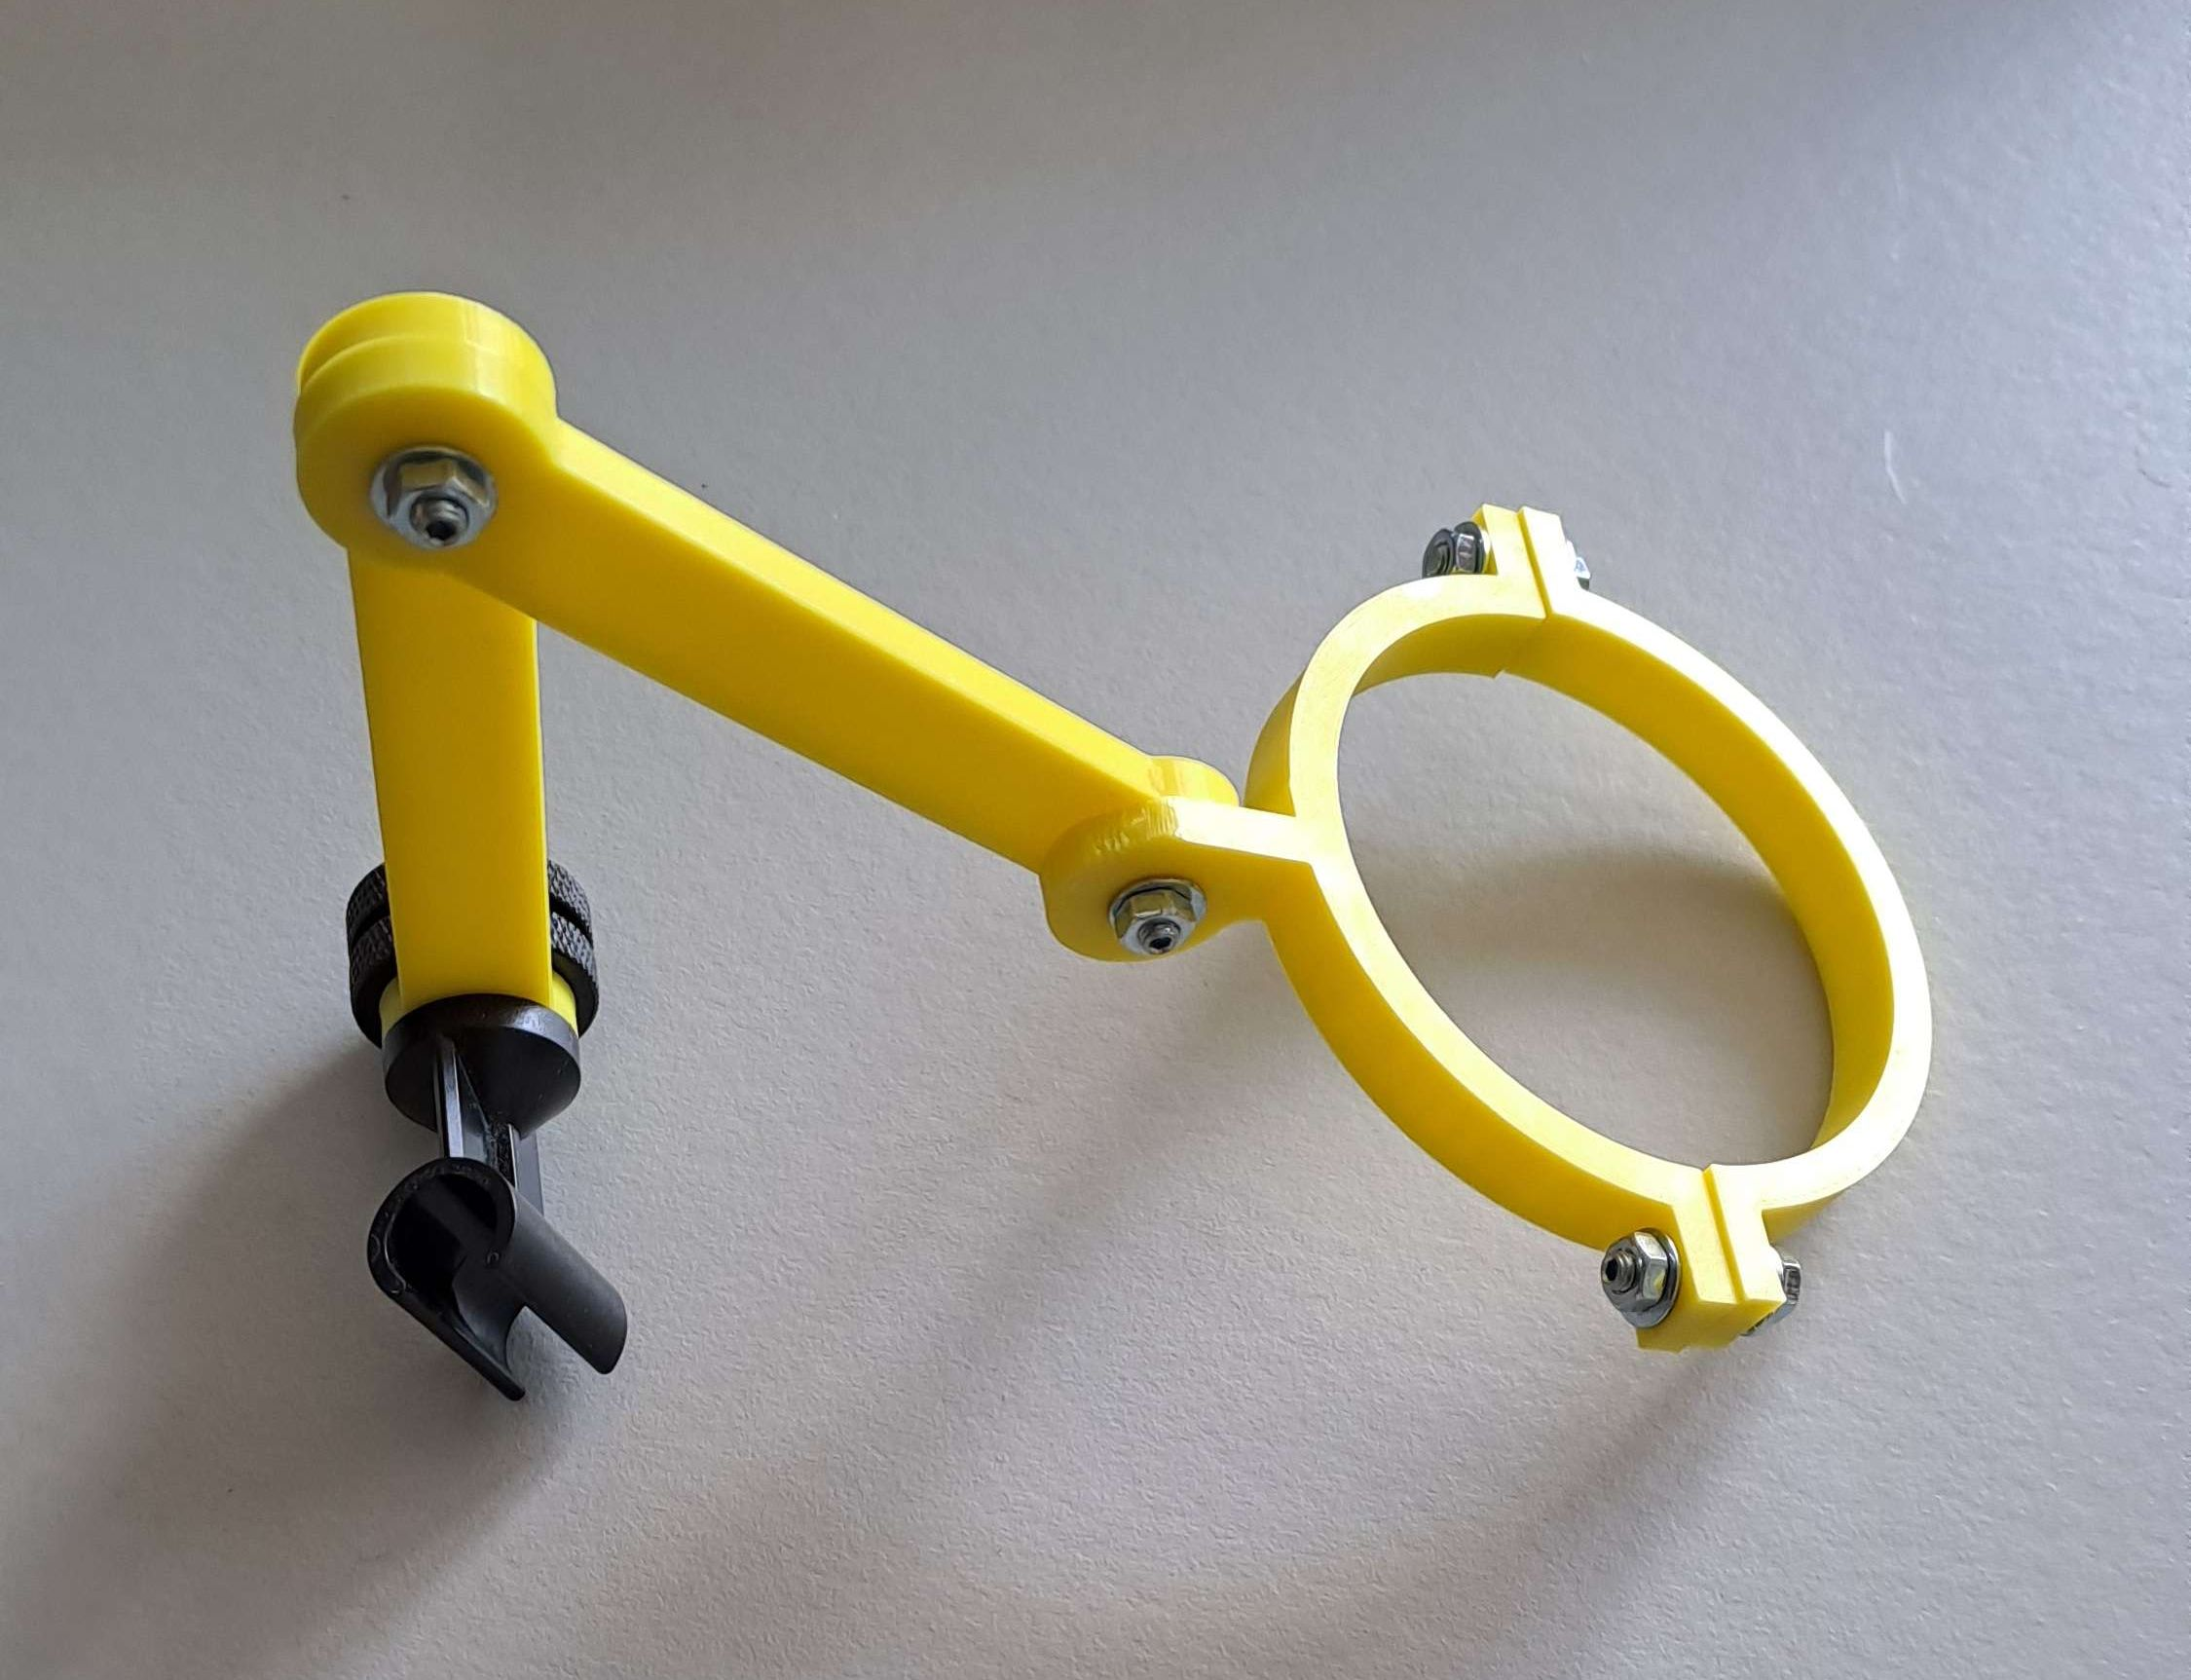
\includegraphics[width=0.5\linewidth]{images/Mikrofonhalterung.jpg}
    \caption{Fertige Mikrofonhalterung}
    \label{fig:Mikrofonhalterung}
\end{figure}

\section{Aufbau}

\begin{figure}[H]
    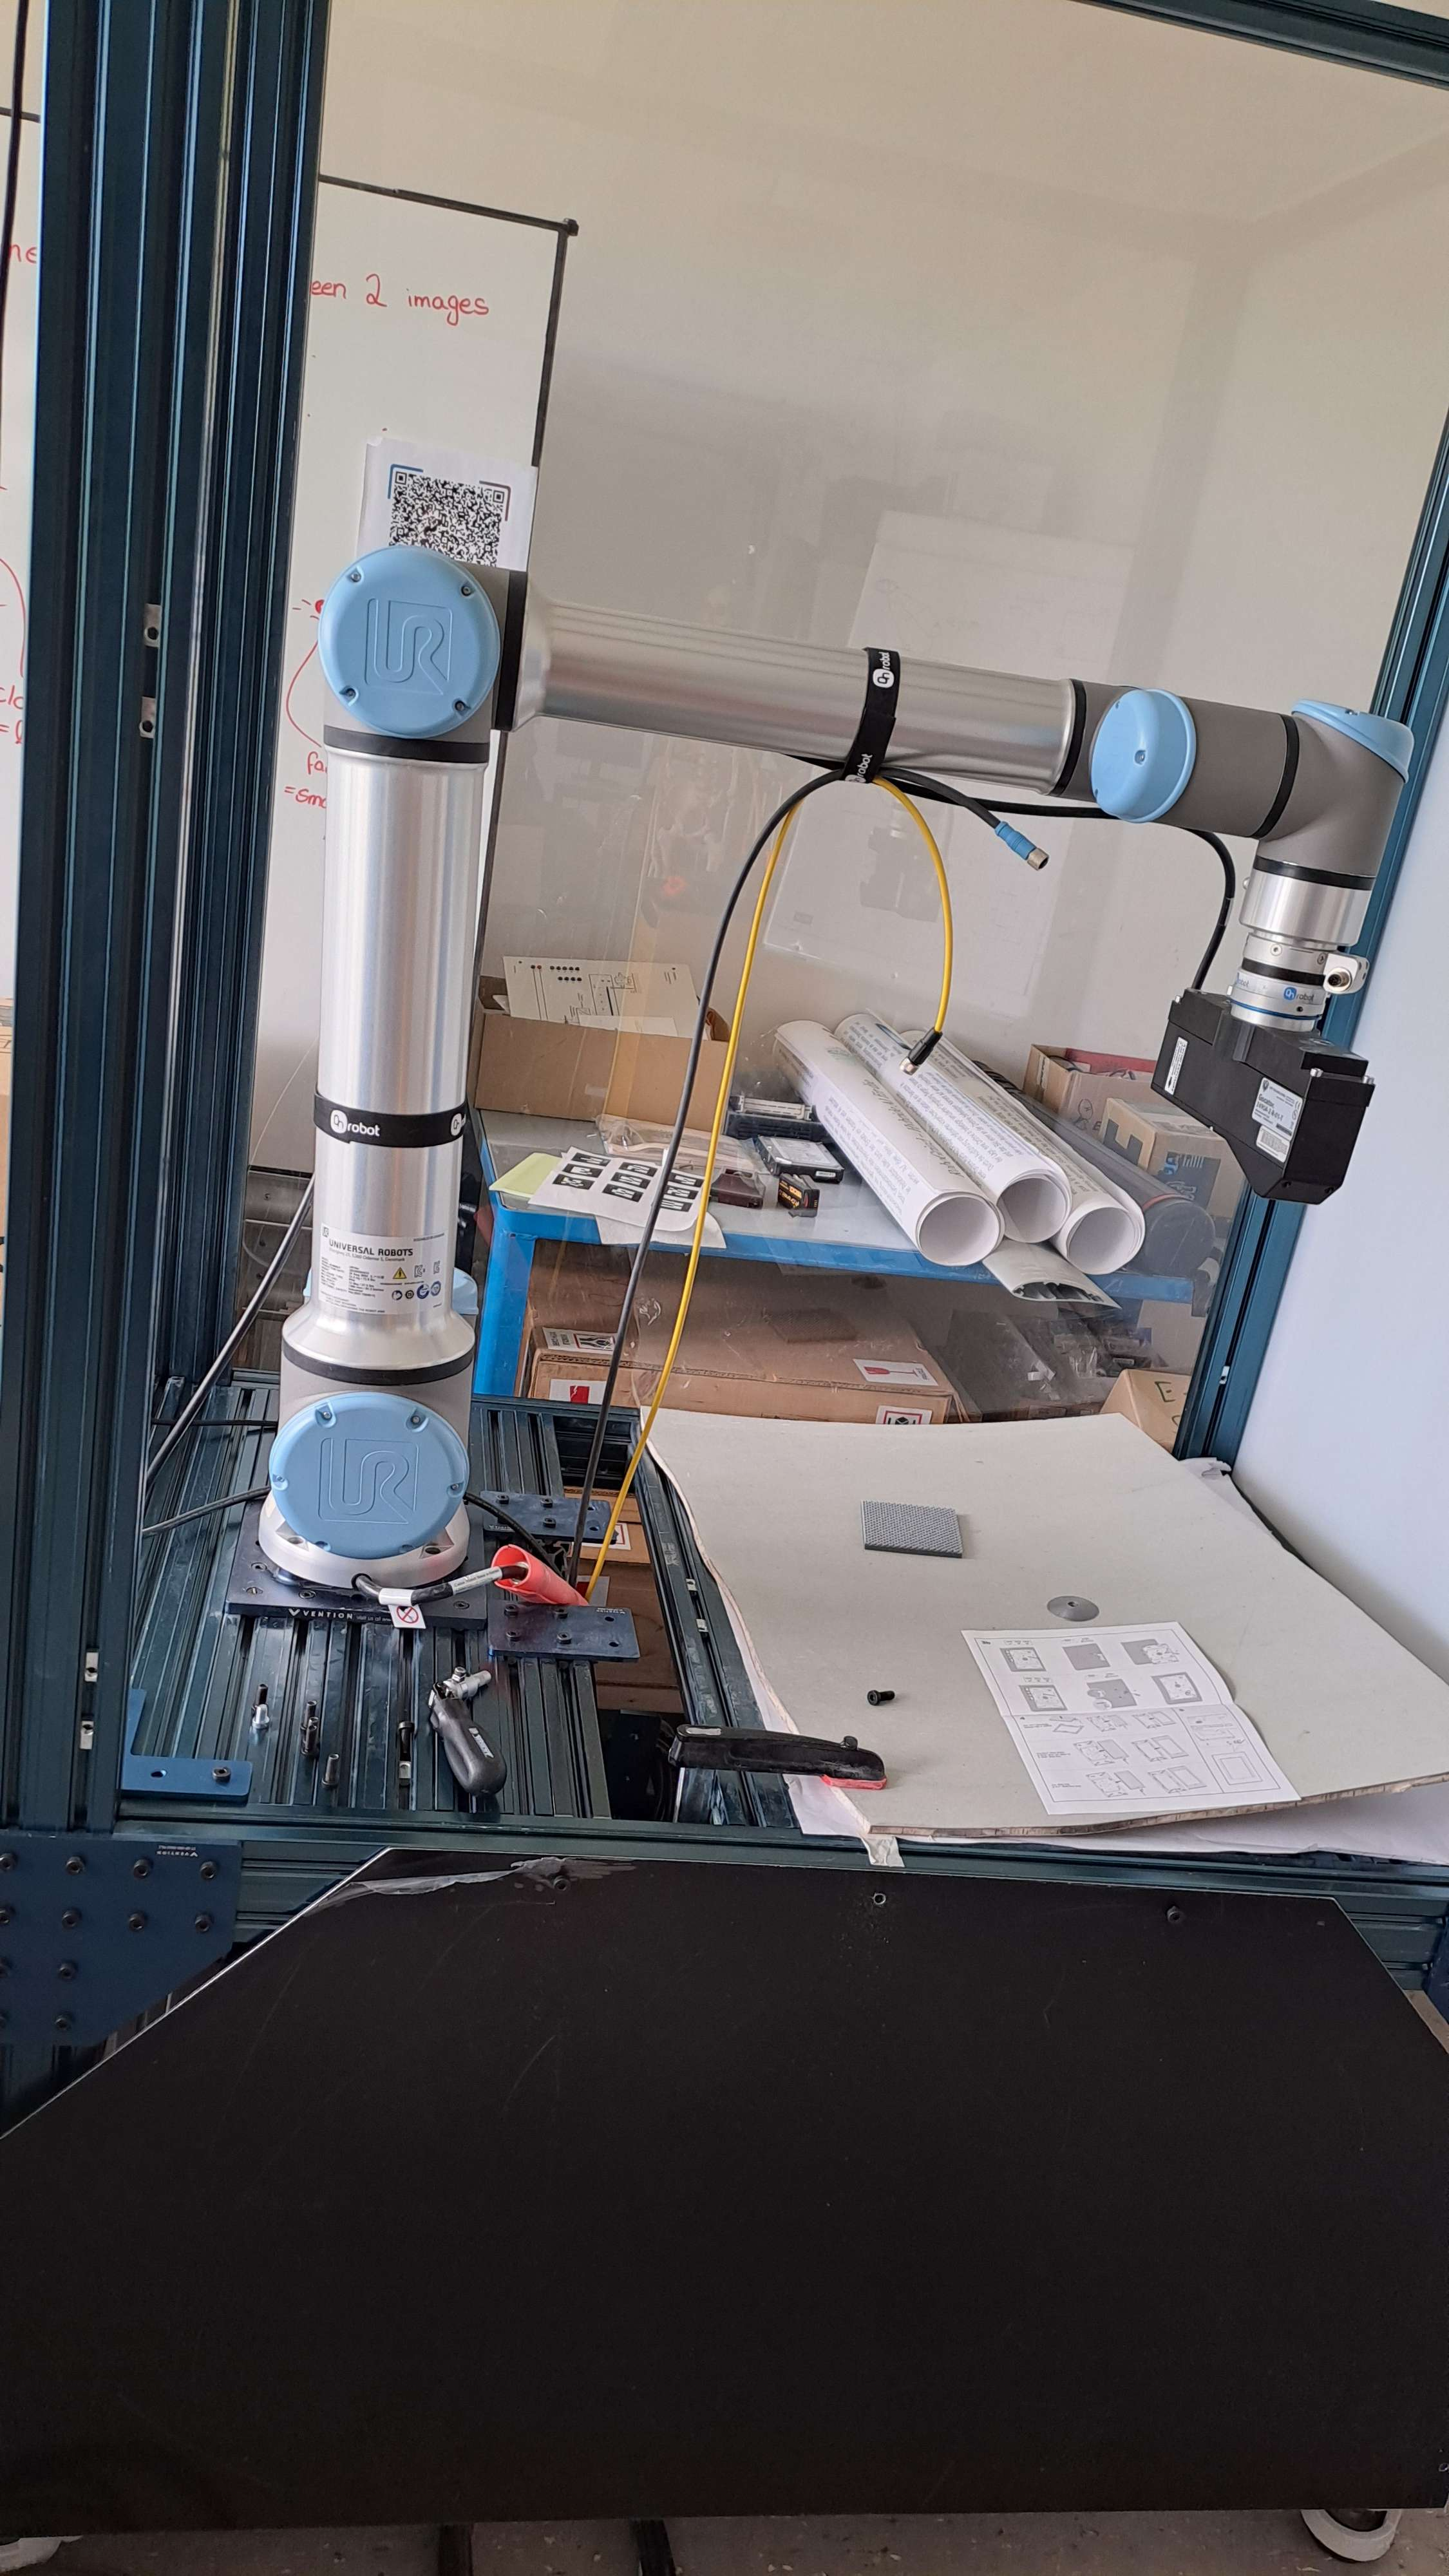
\includegraphics[width=0.5\linewidth]{images/Roboter.jpg}
    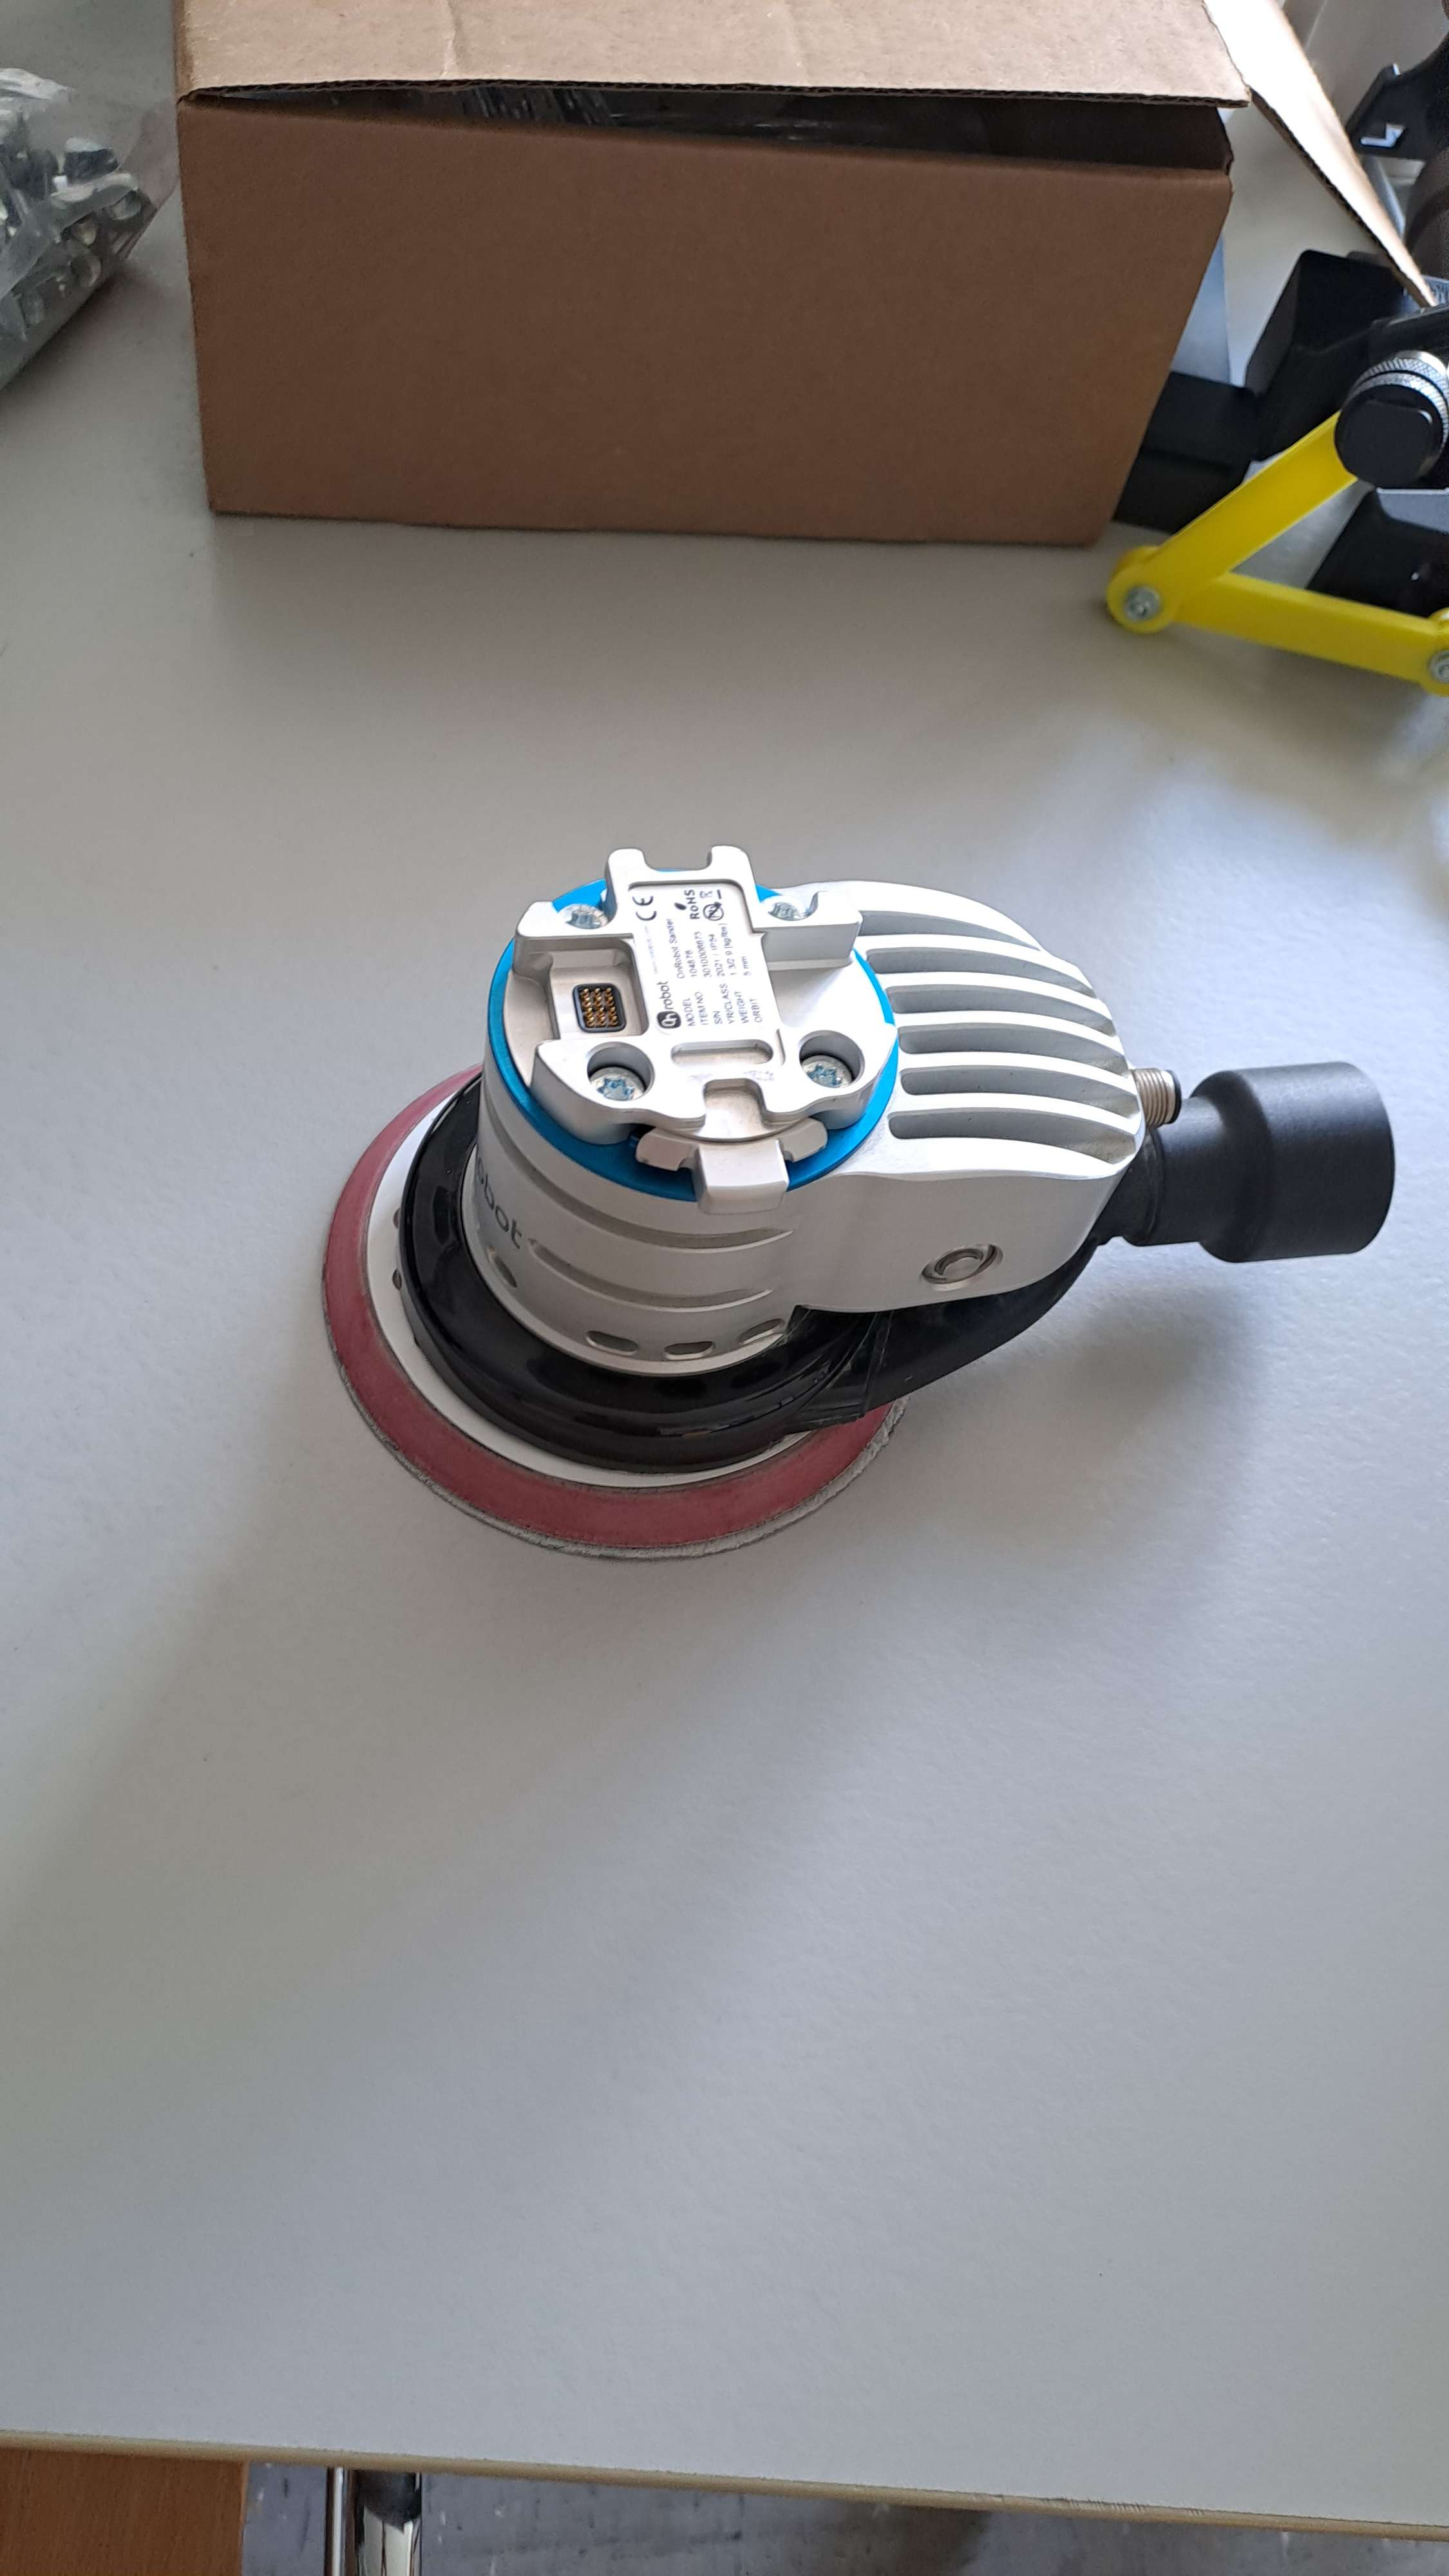
\includegraphics[width=0.5\linewidth]{images/Schleifer.jpg}
    \caption{Roboter und Schleifer}
    \label{fig:Roboter und Schleifer}
\end{figure}

Der Aufbau beinhaltet einen Industrieroboter vom Typ UR10e von Universal Robots. Diese Steuerung des UR10e erfolgt über eine spezielle Software, die es ermöglicht, den Roboter über ein graphisches Benutzerinterface zu programmieren. Diese Software bietet Flexibilität bei der Definition von Bewegungsbahnen, die entweder vorprogrammiert oder während des Betriebs manuell angepasst werden können. Um eine Konsistenz zu gewährleisten wurden mehrere automatische Bahnen programmatisch festgelegt, die den Roboter in definierten Mustern über die Werkstückoberfläche führen. Nach der initialen Konfiguration wurden mehrere Testläufe durchgeführt, um die korrekte Funktion der programmierten Bewegungsbahnen zu überprüfen. Der Roboter operiert innerhalb eines abgeschlossenen Glaskastens, der effektiv den Schleifstaub eingrenzt und den Lärmpegel reduziert, wodurch eine sichere und kontrollierte Arbeitsumgebung gewährleistet wird.

Für den Schleifprozess ist der Roboterarm mit einem OnRobot-104876 Electric Random Orbital Sander ausgestattet, der mittels eines OnRobot-109498 HEX-E Quickchangers befestigt ist. Das verwendete Schleifpapier hat eine Körnung von 120 und war wie neu, ideal für das gleichmäßige Schleifen des Werkstücks, einem Teil eines Windradblattes aus einem Gemisch aus Glasfaser und Holz.

Zur akustischen Überwachung des Schleifvorgangs wurde ein Mikrofon vom Typ M2010 der Marke NTi Audio in einem Abstand von 10-15 mm zum Schleifkopf angebracht. Dieses ist auf dem bereits beschriebenen und in der Abbildung \ref{fig:Mikrofonhalterung} gezeigten 3D gedruckten Mikrofonarm montiert und mit einem Mikrofon-Windschutz (Puschel) ausgestattet, der Störgeräusche wie Luftbewegungen bereits von alleine reduziert.

Die aufgenommenen Audiosignale werden über ein Audiomixer an einen Laptop weitergeleitet, wo sie mit der Software Audacity aufgezeichnet werden. Die Aufzeichnung erfolgt mit einer Abtastrate von 44,1 kHz und einer Bit-Tiefe von 16 Bit, was eine hohe Qualität der Datenerfassung sicherstellt. Diese waren jedoch zu detailliert weswegen diese im Verlauf der Bearbeitung auf 8 kHz Abtastrate heruntergesampelt wurden.

\section{Durchführung}

Bevor der Roboter den Schleifvorgang starten kann, wird der Schleifkopf mit dem passenden Schleifpapier (Körnung 120) bestückt und sicher an der OnRobot-109498 HEX-E Quickchanger-Aufhängung montiert. Anschließend wird das geplante Schleifprogramm auf das Steuerungstablet des UR10e-Roboters geladen und konfiguriert. Hierbei wird insbesondere auf die korrekten Einstellungen für Schleifbahnen, Anpressdruck und Schleifgeschwindigkeit geachtet. Parallel dazu wird die Aufnahmesoftware Audacity auf dem Laptop gestartet. Das Mikrofon wird über Audiomixer an den Laptop angeschlossen. Nachdem die Einstellungen für die Aufnahmesoftware überprüft wurden, wird die Aufnahme gestartet. Dabei wird darauf geachtet, dass die Aufnahmepegel korrekt eingestellt sind, um Übersteuerung zu vermeiden. Sobald die Aufnahme läuft, wird das vorbereitete Schleifprogramm auf dem Roboter gestartet. Der UR10e führt den Schleifprozess entlang der vorgegebenen Bahnen durch und bearbeitet das gebogene Werkstück gleichmäßig mit konstanter Schleifkraft. Die Audiospur in Audacity sieht dann wie folgt aus:

\begin{figure}[H]
    \centering
    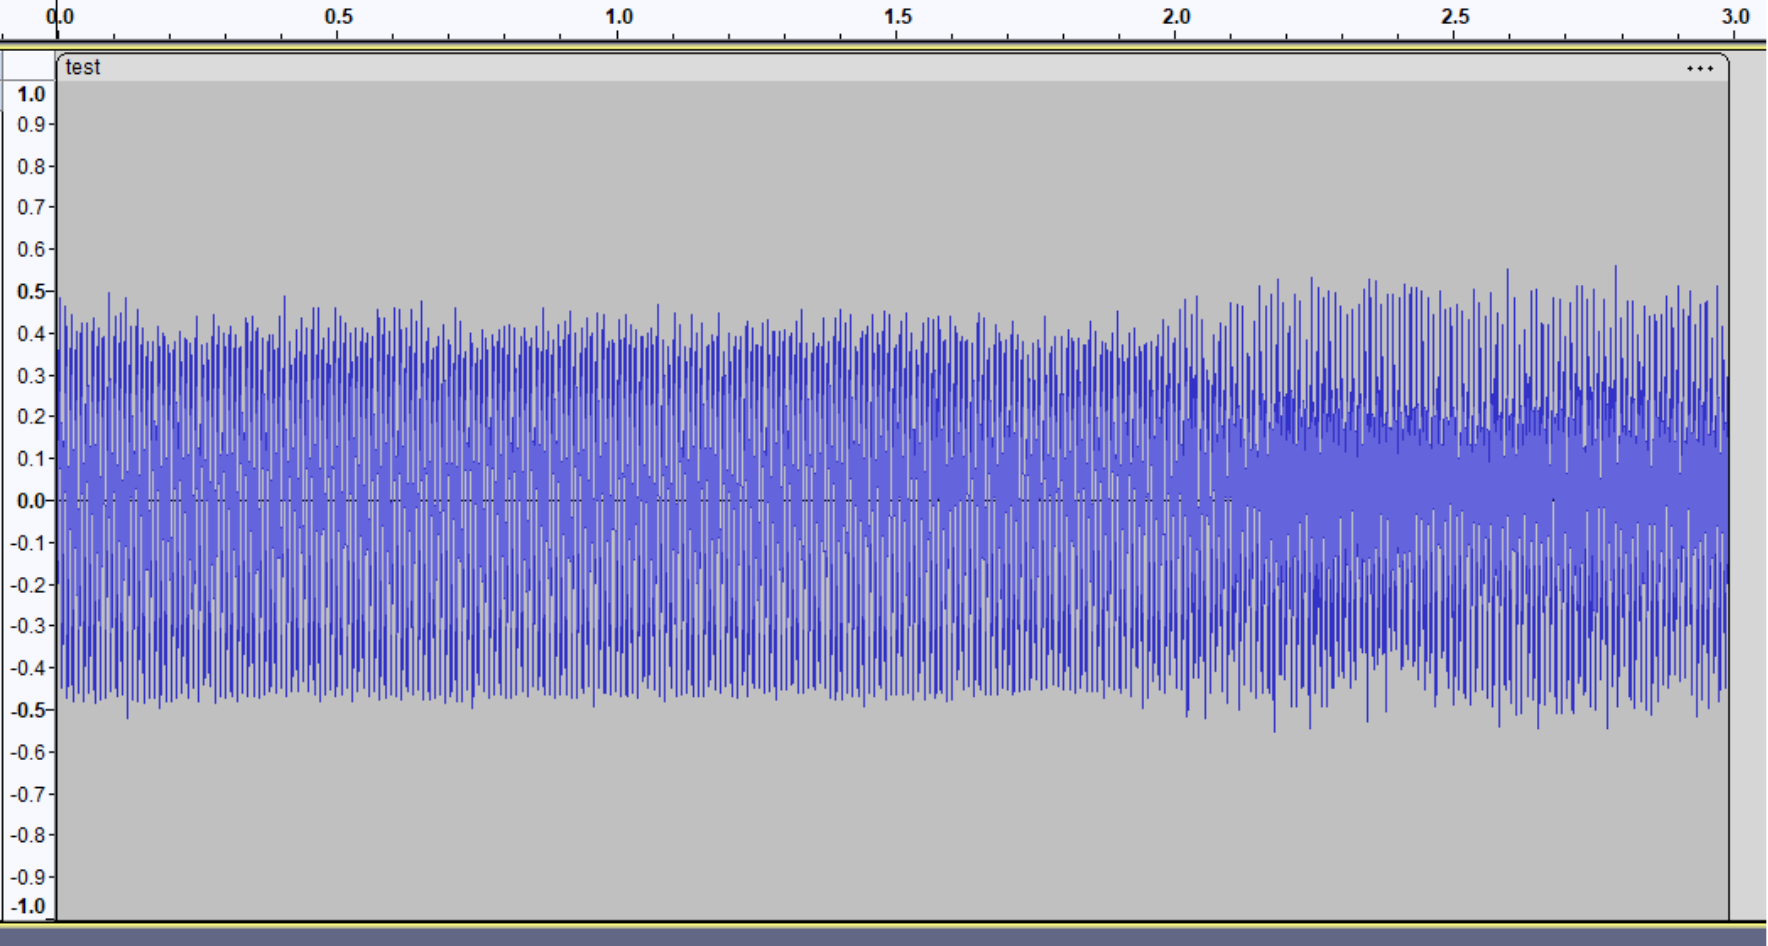
\includegraphics[width=0.7\linewidth]{images/audacity.png}
    \caption{Visualisierung eines Audiosignals in Audacity}
    \label{fig:enter-label}
\end{figure}

Die Aufnahme dauert etwa eine Minute und erfasst den gesamten Schleifvorgang. Sollte während des Schleifens etwas schiefgehen, wie ein zu hoher Anpressdruck, der den Schleifprozess beeinträchtigt, wird die Aufnahme vorzeitig abgebrochen. In diesem Fall wird das Problem identifiziert und behoben, bevor ein neuer Aufnahmeversuch gestartet wird. Nach Abschluss der Aufnahme wird die Audiodatei entsprechend der Einstellungen des Schleifprozesses betitelt und in einer Excel-Tabelle erfasst. Diese Tabelle enthält Informationen zu den verwendeten Schleifprogrammen, Umdrehungszahl, besonderen Ereignissen und weiteren relevanten Parametern, um einen einfachen Überblick über die Aufnahmen zu behalten.     

\section{Auswertung}

Das automatische Schleifen durch vorprogrammierte Bahnen hat nicht immer konsistent funktioniert, da dort mit einer konstanter Kraft nach unten gedrückt wird, was bei einem schrägen Werkstück dazu führt, dass der Schleifer langsam kippt. Bei dem manuellen Schleifen war es allerdings nicht möglich konstistent zu schleifen, da dort die Steuerung deutlich schwieriger ist, was oftmals dazu geführt hat, dass der Anpressdruck bei Beginn des Schleifvorgangs zu hoch war. Weiterhin ist durch die nun nicht mehr automatische Anpressdruckkontrolle dieser über die Breite des Schleifstücks nicht konstant. 

Neben dem Schleifen war auch das Mikrofon anfangs nicht fest genug angebracht, sodass dieses sich durch das Vibrieren des Roboters beim Schleifen langsam abgesenkt hat und somit die Distanz zum Schleifer leicht verändert wurde. Nach erneutem Festziehen der Schrauben war dieses Problem aber gelöst.


%%%%%%%%%%%%%%%%%%%%%%%%%%%%%%%%%%%%%%%%%%%%%%%%%%%%%%%%%%%%%%%%%%%%%%%%%%%%%%%
\endinput
%%%%%%%%%%%%%%%%%%%%%%%%%%%%%%%%%%%%%%%%%%%%%%%%%%%%%%%%%%%%%%%%%%%%%%%%%%%%%%%

\chapter{Auswertung der Audiosignale}
\label{Kapitel6}

Das folgende Kapitel richtet sich nun daran die im vorherigen Kapitel aufgenommenen Daten zu verarbeiten und herauszufinden, welche Informationen aus den aufgenommenen Daten abgelesen werden können. Hierzu wird im ersten Schritt eine \ac{FT} auf die einzelnen Datensätze angewandt. Die Ergebnisse der \ac{FT} können dann ausgewertet werden. Es besteht die Vermutung, dass aus den Frequenzspektren der einzelnen Datensätze bereits einige Informationen extrahiert werden können. Inwiefern diese Vermutung korrekt ist und welche sonstigen Erkenntnisse durch die Anwendung der \ac{FT} getroffen werden können wird nun weiter erläutert. 

\section{FT}
Die Theorie hinter der \ac{FT} wurde bereits erläutert, jedoch ist die Umsetzung dieser Theorie innerhalb von Python-Code komplex. An dieser Stelle verzichten wir darauf die genaue Umsetzung der \ac{FT} zu erläutern, da diese bereits durch die Python-Library scipy erfolgt \cite{scipy-fft}. Wie in der Doku erläutert erfolgt die Berechnung der \ac{FT} durch die scipy-Methode \texttt{fft}. Hierbei handelt es sich um eine Implementierung der \ac{FFT}, welche erheblich schneller umgesetzt werden kann. Da es sich bei unserem Signal zusätzlich um ein reelles und homogenes Signal handelt, wie bereits erläutert, kann auch eine RFFT verwendet werden, welche nur den reellen Teil (R) des Signals betrachtet. Durch die Methode \texttt{rfftfreq} lassen sich zusätzlich die Frequenzen berechnen, welche notwendig sind, um das Ergebnis als Frequenzspektrum zu plotten. Um das Ergebnis zu plotten wird die Python-Library matplotlib genutzt. \cite{matplotlib} Mithilfe dieser beider Librarys lassen sich jetzt die Frequenzspektren der einzelnen Signale plotten. 

Die Abbildung \ref{fig:frequenzspektren-fft} zeigt nun exemplarische Frequenzspektren für verschiedene Konfigurationen. Das Keyword ,,Air'' steht hierbei dafür, dass das gezeigte Signal aufgenommen wurde, als der Schleifer in der Luft war, Signalen mit dem Keyword ,,Grinding'' wurden während eines vermeintlichen Schleifprozesses aufgenommen. Die Zuordnung dieser Keywords erfolgt manuell, dadurch kann es Signale mit dem Keyword ,,Grinding'' geben, bei welchem nicht wirklich geschliffen wurde. Genau diese manuelle Zuweisung des Keywords soll durch diese Arbeit automatisiert werden. Zusätzlich enthalten die Abbildungen die Information über die beim Roboter ansteuern festgelegten RPM. Diese festgelegten RPM können als SOLL angesehen werden, das Ziel dieser Arbeit wiederum ist es den IST-Wert der RPM automatisiert zu berechnen. 

\begin{figure}[H]
    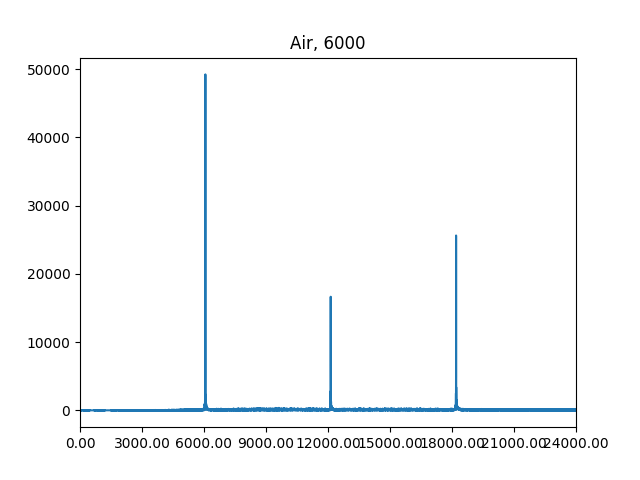
\includegraphics[width=0.5\linewidth]{Studienarbeit//images/Air, 6000, FFT.png}    
    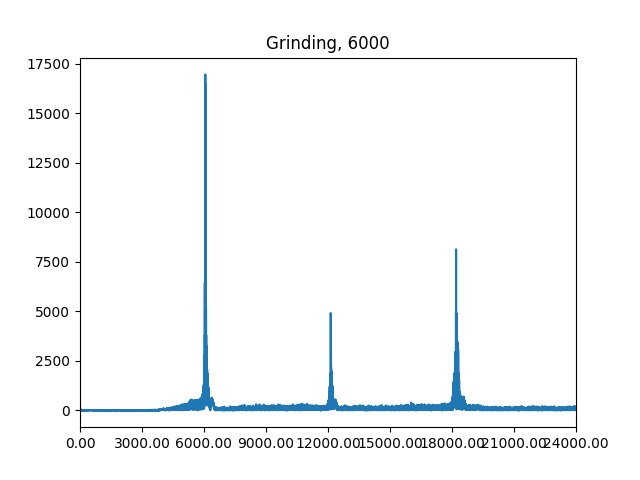
\includegraphics[width=0.5\linewidth]{Studienarbeit//images/Grinding, 6000, FFT.png}
    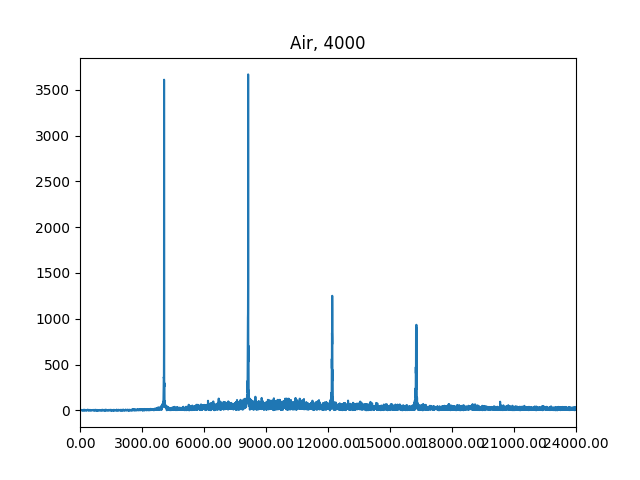
\includegraphics[width=0.5\linewidth]{Studienarbeit//images/Air, 4000, FFT.png}
    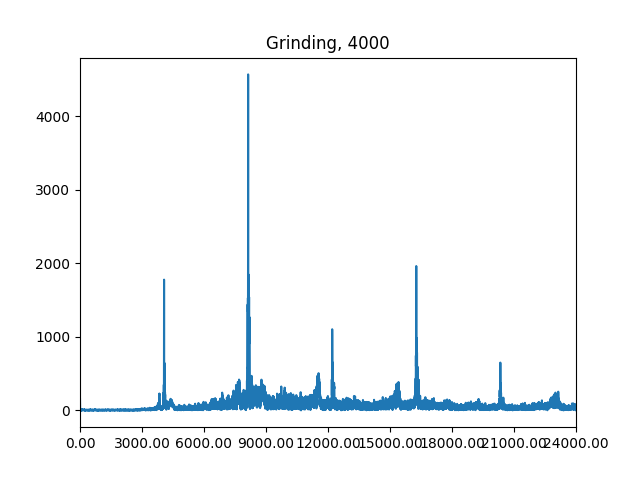
\includegraphics[width=0.5\linewidth]{Studienarbeit//images/Grinding, 4000, FFT.png}
    \caption{Frequenzspektren verschiedener Signale}
    \label{fig:frequenzspektren-fft}
\end{figure}

Die erste Annahme ist, dass der höchste Peak im Frequenzspektrum mit der verwendeten RPM korreliert, da sowohl der Schleifer als auch der Motor Geräusche in diesem Frequenzbereich erzeugen sollten. Wenn man diese Annahme weiterführt, sollten sich bei jedem vielfachen dieser korrelierenden Frequenz ebenfalls ein Peak befinden. Beim betrachten der Abbildungen fällt nun auf, dass dies nicht überall der Fall ist. So ist deutlich zu erkennen, dass diese Annahme bei 6000RPM erfüllt ist, bei 4000RPM ist der höchste Peak jedoch bei 4000 RPM. Stattdessen befindet sich der höchste Peak bei 8000RPM also der doppelten Drehzahl. Woher genau dieser Peak stammt konnte nicht herausgefunden werden, es besteht allerdings die Vermutung, dass durch die 4000 RPM eine Eigenschwingung angeregt wird. Des Weiteren ist es möglich, dass die benutzte Technik hier Probleme aufweist. Um jetzt diese RPM auszulesen bietet es sich an eine Methode zu schreiben, welche alle diese Daten durchgeht und immer dann ein Peak als solchen identifiziert, wenn ein vorher festgelegter Grenzwert überschritten wird. Betrachten wir jedoch die beiden oberen Frequenzspektren fällt auf, dass die Amplitude der Frequenzen sehr unterschiedlich sein kann, so ist es nicht möglich  für jedes Signal den gleichen Grenzwert verwenden kann. Um dies zu beheben müssten nun die Amplituden der Signale normalisiert werden. Diese Normalisierung wird an dieser Stelle zunächst nicht durchgeführt, da durch die bereits aufgeführten Grundlagen die Vermutung auftritt, dass dieses Problem sich durch die Verwendung einer \ac{STFT} oder einer \ac{CWT} lösen lässt. Als Ergebnis lässt sich hier an dieser Stelle bereits festhalten, dass sie die RPM des 6000 gut herauslesen lassen und mit mehr Aufwand bereits dies bereits bei der \ac{FFT} möglich wäre. Das einfache Ablesen durch eine Methode bei 4000RPM ist dies jedoch nicht möglich, da der höchste Wert nicht die RPM widerspiegelt.

Die zweite Eigenschaft, die durch diese Arbeit automatisiert heraus gelesen werden sollte ist die Erkennung, ob der Schleifer tatsächlich geschliffen hat oder die Schleifleistung nicht wie erwartet erfolgt ist. Betrachten wir uns wieder die Abbildung \ref{fig:frequenzspektren-fft} sehen wir, dass die Frequenzspektren der Signale mit der Angabe ,,Grinding'' viel mehr kleinere Spikes besitzen. Auch hier fällt wieder auf, dass bei 4000RPM auch in der Luft das Frequenzspektren viele kleine Spikes aufweist, dies verstärkt wiederum die Vermutung, dass irgendwas die Frequenzen dort verstärkt und verrauscht. Um nun automatisiert zu ermitteln, ob in dem vorhandenen Datensatz geschliffen wurde, könnte man auch hier eine Methode implementieren, welche die Anzahl der Peaks zählt und einen Grenzwert festlegen, ab welchem ein vorliegendes Signal mit dem Zusatz ,,Grinding'' klassifiziert wird. Eine Alternative dazu ist die Ermittlung des Signal-Rausch-Verhältnis des Frequenzspektrum, wenn nun das SNR berechnet wurde, kann auch hier ein Grenzwert festgelegt werden. Bei diesen beiden Grenzwerten tritt ähnlich wie bei der Festlegung des Grenzwertes für die RPM Bestimmung das Problem auf, dass sich der Grenzwert hier für jedes Signal Unterscheiden kann. An dieser Stelle stellt sich auch die Vermutung auf, dass dieses Problem durch die Nutzung einer \ac{STFT} oder \ac{CWT} gelöst werden kann, da durch die \ac{STFT} und die \ac{CWT} das Signal besser normalisiert wird.

Zusammenfassend lässt sich an dieser Stelle sagen, dass es den Anschein erweckt, dass aus den vorliegenden Daten Informationen über die RPM und die Schleifleistung extrahiert werden können. Diese Daten könnten vielleicht durch die Entwicklung komplexer Algorithmen für die Grenzwertfestlegung der Amplitude, der Peakanzahl und für das SNR berechnet werden. Die Implementierung dieser Methoden erfolgt an dieser Stelle aber zunächst nicht, da die Vermutung besteht, dass durch die Anwendung einer \ac{STFT} oder \ac{CWT} die gewünschten Informationen schneller und weniger komplex ausgelesen werden können, da bei beiden das Eingangssignal durch die Beibehaltung der zeitlichen Komponente besser normalisiert werden kann. Durch diese Normalisierung, können dann mehr unterschiedliche Signale analysiert werden, wodurch die Fehleranfälligkeit sinken würde. Um diese Vermutung zu überprüfen erfolgen nun in den nächsten Unterkapiteln die Durchführung einer \ac{STFT} und einer \ac{CWT}, mit dem Ziel Informationen über die RPM und die Schleifleistung mit einer höheren Zuverlässigkeit bereitstellen zu können.


\section{STFT}
Dieses Kapitel richtet sich nun daran die Audiosignale mithilfe einer \ac{STFT} zu analysieren. Die Grundlagen, wie eine solche \ac{STFT} funktioniert wurde schon bereits erläutert. Die Phyton Implementierung der \ac{STFT} findet durch die bereits für die \ac{FT} verwendete Phyton-Library scipy statt. Diese Implementierung basiert auf dem vorgestellen Algorithmus von Cooley und Tukey \cite{scipy-stft}. Um nun \ac{STFT} mit dieser Bibilothek durchführen zu können muss zunächst das Fenster festgelegt werden, welches danach Schritt für Schritt über das Signal gelegt werden kann. Zusätzlich muss der Versatz festgelegt werden. Um trotz der Überlappung möglichst viele Informationen extrahieren zu können bietet es sich an ein nicht lineares Fenster zu benutzen. Ein weit verbreitetes Fenster ist das Gaussian-Fenster, welches Glockenförmig ist und somit Daten in der Mitte des Fensters eine höhere Gewichtung gibt. Diese höhere Gewichtung ist sinnvoll, da die Daten am Rand des Fensters durch die Überlappung doppelt ausgewertet werden. Zusätzlich lässt sich bei diesem Gaussian-Fenster die Standardabweichung festlegen, welche die Glocken-breite bestimmt. Die Form und Länge des Fensters bestimmt das Ergebnis der \ac{STFT}, um herauszufinden, welche Parameter für den spezifischen Anwendungsfall am besten geeignet sind, müssen verschiedene Parameter verglichen werden.

\paragraph{Parameterwahl}
Die Abbildung \ref{fig:parameter-stft} zeigt die Anwendung verschiedener Versätze (\(\Delta t\)) und Fenster-Längen und Standardabweichungen des Gaussian-Fenster (\(\sigma\)) zu erkennen. Hierbei wurde als Signal mit 6000RPM und der Klassifizierung ,,Air'' gewählt und der Länge von 60s gewählt.

\begin{figure}[H]
    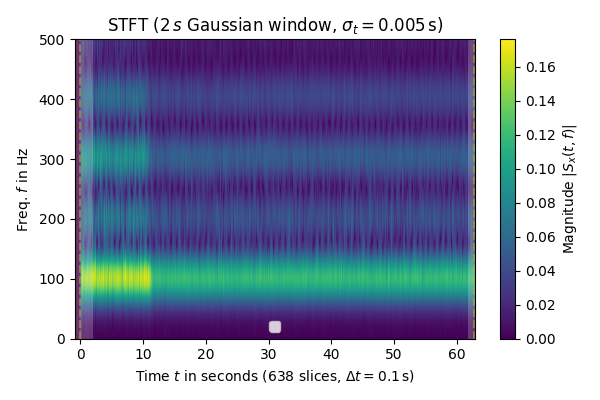
\includegraphics[width=0.5\linewidth]{Studienarbeit//images/2sr-1_400-sr_10.png}    
    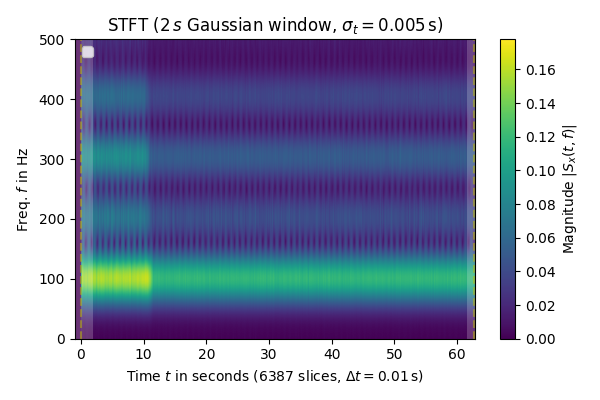
\includegraphics[width=0.5\linewidth]{Studienarbeit//images/2sr-1_400-sr_100.png}
    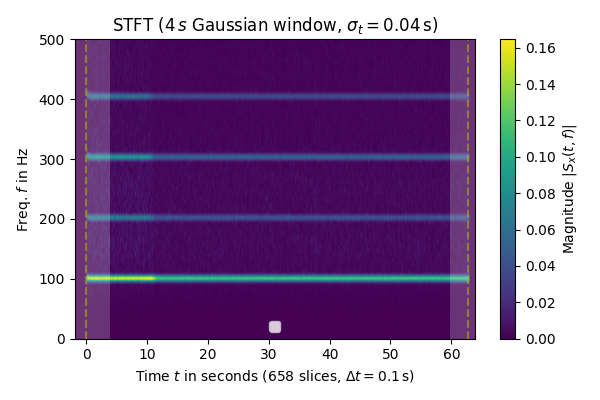
\includegraphics[width=0.5\linewidth]{Studienarbeit//images/4sr-1_100-sr_10.png}
    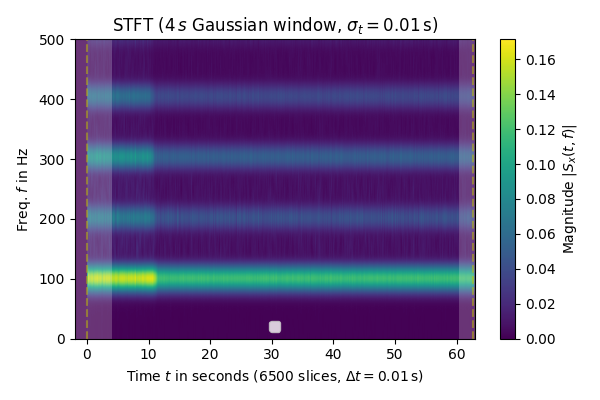
\includegraphics[width=0.5\linewidth]{Studienarbeit//images/4sr-1_400-sr_100.png}
    \caption{Auswirkung verschiedener Parameter auf die STFT}
    \label{fig:parameter-stft}
\end{figure}

Wie bereits im Grundlagen Kapitel \ref{Kapitel2} erläutert muss man sich je nach Anwendungsfall für Zeit- oder Frequenzgenauigkeit entscheiden, da bereits durch die \ac{FFT} auffällt, dass die Schleifgeräusche nicht besonders deutlich zu erkennen sind, scheint hier eine Fokussierung auf die Frequenzgenauigkeit sinnvoll, um die wenigen Informationen die man hat möglichst detailiert auszuwerten. Wie in der Abbildung \ref{fig:parameter-stft} erkennbar erreicht man eine diese durch die Verlängerung des Fensters. So sind die Frequenzen viel detaillierter in den beiden unteren Abbildungen mit einer Fenstergröße von 4s zu erkennen, als bei 2s. Eine noch höhere Genauigkeit wird durch die Vergrößerung der Standardabweichung \(\sigma\) erreicht, zu erkennen in den unteren Bildern. Zusätzlich erhöht sich jedoch die Zeitliche Genauigkeit durch Verringerung des Versatzes (\(\Delta t\) auf der X-Achse). Da besonders der Fokus auf die Frequenzen notwendig ist, wird sich an dieser Stelle für eine Fenstergröße von 4s entschieden, dies der 4-fachen sampling-rate entspricht. Zusätzlich wird ein Versatz von 0,1s, also 1/10 der sampling-rate als sinnvoll betrachtet. Für die Standardabweichung wird sich für 0,04s entschieden, dies entspricht 1/100 der Fensterbreite. Diese Wahl der Parameter sorgt dafür, dass die Frequenz und deren Schwankungen sehr genau abgebildet werden und trotzdem noch genügend Informationen vorhanden sind, um zeitliche Angaben zu treffen.

\paragraph{Auswertung verschiedener Datensätze}
Da nun die Wahl der Parameter erfolgt ist, werden nun verschiedene Datensätze mithilfe einer \ac{STFT} und diesen gewählten Parametern ausgewertet. Die Abbildung \ref{fig:verschiedene-stft} zeigt mehrere repräsentative Ergebnisse. Die Beschriftungen der Abbildungen ist wie auch bei der \ac{FFT} gewählt.

\begin{figure}[H]
    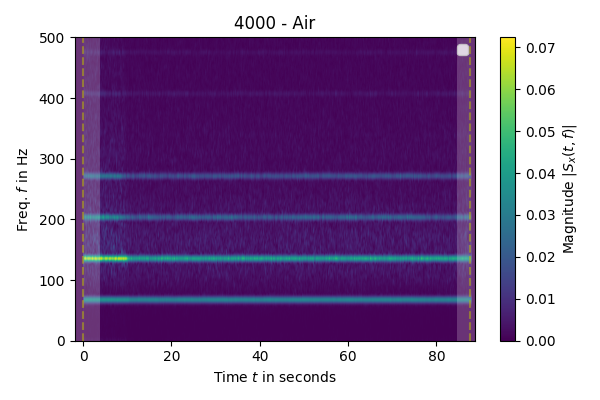
\includegraphics[width=0.5\linewidth]{Studienarbeit//images/stft-4000-air.png}    
    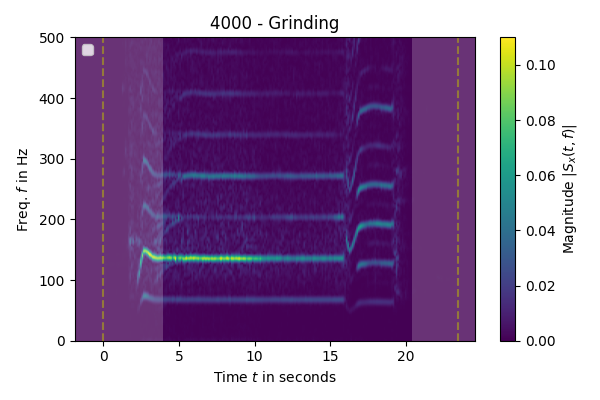
\includegraphics[width=0.5\linewidth]{Studienarbeit//images/stft-4000-grinding.png}
    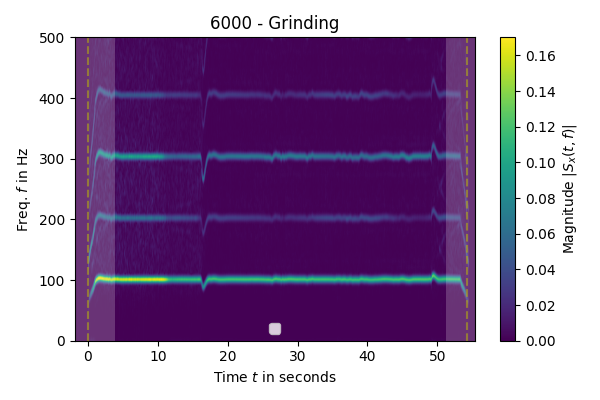
\includegraphics[width=0.5\linewidth]{Studienarbeit//images/stft-6000-grinding.png}
    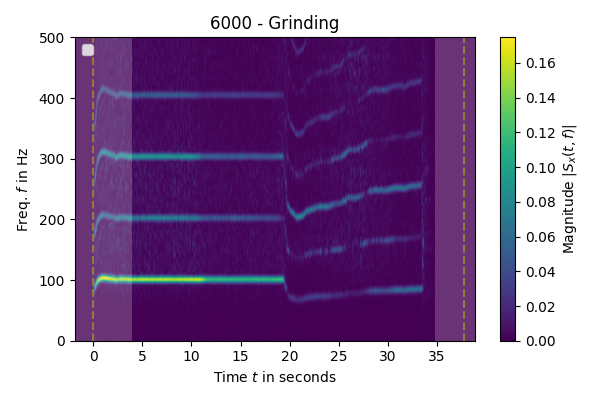
\includegraphics[width=0.5\linewidth]{Studienarbeit//images/stft-6000-grinding-hard.png}
    \caption{Anwendung der STFT auf verschiedene Signale}
    \label{fig:verschiedene-stft}
\end{figure}

Ähnlich wie auch bei der \ac{FFT} ist in den Abbildungen deutlich zu erkennen, dass eine Frequenz stärker heraus sticht, als die anderen. Bei einem SOLL von 4000 RPM sticht die Frequenz von \textasciitilde 130Hz besonders hervor, 130HZ entsprechen hier \textasciitilde 8000RPM. Das verstärkte Auftreten der doppelten Frequenz bei SOLL-4000RPM wurde bereits bei der \ac{FFT} beobachtet. Die Gründe dafür bleiben weiter unbekannt. Da diese Verstärkung jedoch immer auftritt und auch über die gesamte Audiolänge hinweg, kann davon ausgegangen werden, dass dies vom Motor des Schleifers selbst stammt. Bei den SOLL von 6000RPM liegt die gemessene Frequenz bei \textasciitilde 100HZ, was wiederum 6000RPM entspricht. Da dieser Peak konstant zu sein scheint, lässt sich daraus die IST-RPM berechnen, mehr dazu im nächsten Abschnitt. Vorher betrachten wir die beiden rechten Abbildungen. Bei beiden ist am Ende eine Verwischung der Frequenzen zu erkennen. Interessant hierbei ist, dass beim Aufnehmen dieser beiden Audiospuren der Schleifer am Ende zu stark auf das Material gedrückt hat. So stellt sich hier die Vermutung auf, dass es sich bei der zu sehenden Anomalie um einen zu hohen Anpressdruck handelt. Diese Vermutung wird an späterer Stelle nochmals aufgegriffen. Eine weitere zu erkennende Anomalie ist, dass in jedem Audiosignal in den ersten 10 Sekunden die Frequenzen stärker ausgeprägt scheinen. Ein Grund dafür lässt sich auch nur vermuten, aber da die Frequenz hierbei konstant bleibt und der Zeitraum der Verstärkung immer am Anfang der Aufnahme liegt, liegt die Vermutung nahe, dass es sich möglicherweise um Resonanzen im Aufnahmesystem oder elekrisches Rauschen handelt. Da dieses Rauschen in jedem Audiosignal gleich stark aufzutreten scheint, kann dies vernachlässigt werden.

Um nun die RPMs berechnen zu können wird eine Methode implementiert, welche die maximale Ausprägung einer Frequenz findet. Da durch die \ac{STFT} auch eine zeitliche Komponente enthalten ist, liegt die Entscheidung nahe die RPMS nicht für die gesamte Audiospur, sondern immer für kleine Teile zu berechnen. Im Sinne der reellen Anwendung scheint hierbei eine Auswertung auf Sekunden-ebene sinnvoll. Nachdem die am stärksten ausgeprägte Frequenz gefunden wurde lässt sich diese mit 60 multiplizieren um RPMs zu erhalten. Der Algorithmus geht also Sekunden-weise durch die Ergebnisse der \ac{STFT} durch und sucht immer die am stärksten ausgeprägte Frequenz. Die Abbildung \ref{fig:rpm-stft} zeigen nun die berechneten RPMs für die in der Abbildung \ref{fig:verschiedene-stft} gezeigten Datensätze, zusätzlich ist auf den Diagrammen die Stärke der Ausprägung (Intensity) angegeben, zur Veranschaulichung ist diese Ausprägung mit einem Faktor von 100000 multipliziert.

\begin{figure}[H]
    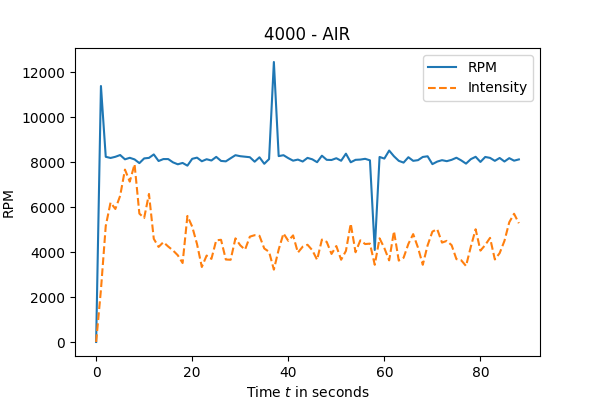
\includegraphics[width=0.5\linewidth]{Studienarbeit//images/stft-rpm-4000-air.png}    
    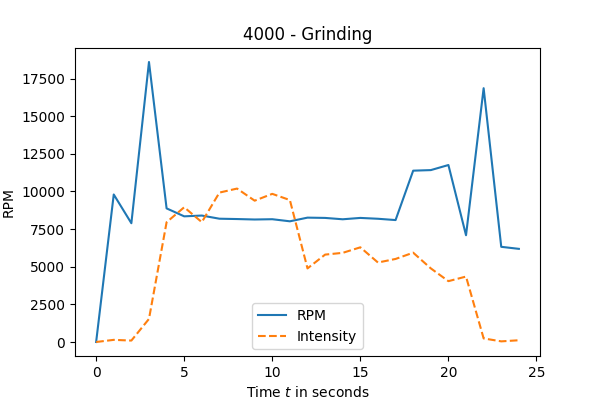
\includegraphics[width=0.5\linewidth]{Studienarbeit//images/stft-rpm-4000-grinding.png}
    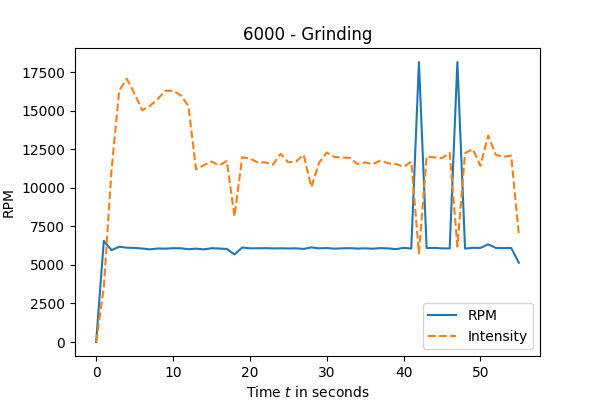
\includegraphics[width=0.5\linewidth]{Studienarbeit//images/stft-rpm-6000-grinding.png}
    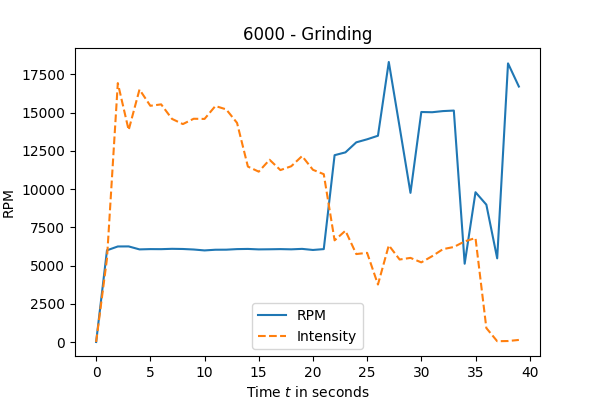
\includegraphics[width=0.5\linewidth]{Studienarbeit//images/stft-rpm-6000-grinding-hard.png}
    \caption{Berechnung der RPM durch die STFT}
    \label{fig:rpm-stft}
\end{figure}

Wie bereits erwartet und auch sowohl bei der \ac{FFT} als auch bei der \ac{STFT} sichtbar, weißt die berechnete RPM bei SOLL-4000 eine Abweichung auf und es wird ein IST von 8000 RPM berechnet. Die Quelle für dieses akustische Rauschen in den Audiosignalen im Bereich von 4000 RPM konnte jedoch nicht gefunden werden, es besteht weiterhin die Vermutung, dass es sich hierbei um ein Rauschen handelt, welches durch die Eigenfrequenz des Schleifers ausgelöst wird. Für die Datensätze mit einem SOLL von 6000 RPM erzielt die Methode gute Ergebnisse, jedoch gibt es auch hier Abweichungen. So treten immer dann Abweichungen auf, wenn in der \ac{STFT} Anomalien auftreten, welche vielleicht auf die Schleifleistung zurückzuführen sind, zu sehen in den linken Plots. Interessant ist auch die Intensität der RPM, so ist die Intensität bei den mit ,,Grinding'' markierten Diagrammen immer dann höher, wenn auch die korrekte IST-RPM berechnet wurde. Bei den in der Luft aufgenommenen Datensätzen ist die Intensität auch niedriger. Daraus lässt sich die Vermutung aufstellen, dass die Intensität während der Erbringung einer guten Schleifleistung höher ist. Sinkt die Intensität, so steigt oder sinkt der Anpressdruck so stark, dass die Schleifleistung beeinträchtigt wird. Einen wirklichen Grenzwert lässt sich hierfür jedoch nicht festlegen.

Insgesamt lässt sich an dieser Stelle festhalten, dass es teilweise möglich ist die richtigen RPM zu berechnen, jedoch ist diese Berechnung fehleranfällig. Zusätzlich lassen sich aus den Plots Vermutungen über die Schleifleistung aufstellen. Dennoch haben wir uns entschieden den Ansatz der \ac{STFT} nicht weiter zu Verfolgen. Die \ac{STFT} hat ihren Zweck in der Arbeit erfüllt, in dem Sinne, dass durch die Anwendung aufgezeigt wurde, dass die zeitliche Komponente in diesem Anwendungfall wichtig ist, zusätzlich hat es Beweise dafür geliefert, dass in den Daten Informationen über die RPM und die Schleifleistung enthalten sind. Durch das analysieren vorhandener State-of-the-Art Methoden im Kapitel \ref{Kapitel3} wurde aufgezeigt, dass es eine Methode gibt, welche zwar teilweise komplizierter zu implementieren ist, jedoch im direkten Vergleich wesentlich detailliertere Ergebnisse liefert. Die Rede ist von der \ac{CWT}. Dies ist der Hauptgrund dafür, dass wir uns an dieser Stelle uns dafür entscheiden nicht tiefer die Ergebnisse der \ac{STFT} zu analysieren und stattdessen die grobe Ergebnisse als Machbarkeitsbestätigung zu interpretieren und die genaueren Analysen mithilfe der \ac{CWT} durchzuführen. 


\section{Auswertung mithilfe von CWT}
Wie bereits erwähnt, findet nun die Auswertung mithilfe der \ac{CWT} statt. Hierfür verwenden wir eine auf \cite{Torrence1998} basierende Python-Bibliothek, welche bereits im Kapietel \ref{Kapitel3} ausführlich erläutert wurde. Die wichtigsten Punkte werden hier nun nochmal zusammengefasst.

Um verschiedene Frequenzen isolieren zu können, werden die oben genannten Audiospuren mithilfe einer Wavelet-Transformation analysiert. Dabei verwenden wir das Morlet Wavelet, wobei die Transformation unter der Verwendung einer in \cite{Torrence1998} vorgestellten Methode im Fourier-Raum erfolgt. Wie bereits in Kapitel \ref{Kapitel3} gezeigt, besteht das Morlet-Wavelet aus einer komplexen Exponentialfunktion, die von einer Gauß'schen Funktion moduliert wird \(e^{i\omega_0 t/s}e^{-t^2/(2s^2)}\), wobei \(t\) die Zeit, \(s\) die Skalierung des Wavelets und \(\omega_0\) eine dimensionslose Frequenz ist. Als Erweiterung zu einer einfachen \ac{CWT} nutzt die Bibilothek einen Signifikanz-Test, welcher die Peaks im Wavelet-Powerspektrum betont. Um die Signifikanz zu testen, muss ein Hintergrund-Fourier-Spektrum gewählt werden. Um nicht stationäre Änderungen in der Varianz zu testen, ist es am besten, das globale Wavelet-Spektrum (GWS) zu wählen, das sich aus dem Zeitdurchschnitt des Wavelet-Leistungsspektrums ergibt. Das Wavelet-Leistungsspektrum ist dann um das GWS (Verteilung als Chi-Quadrat mit zwei Freiheitsgraden) verteilt. Zusätzlich wird ein Filter festgelegt, damit einzelne Frequenzbereiche besser isoliert betrachtet werden können. Die Abbildung \ref{fig:cwt-filter} zeigen nun die Anwendung dieses Filters auf das GWS. Gezeigt wird ein Red-Noise-Filter und dessen inverse.

\begin{figure}[H]
    \centering
    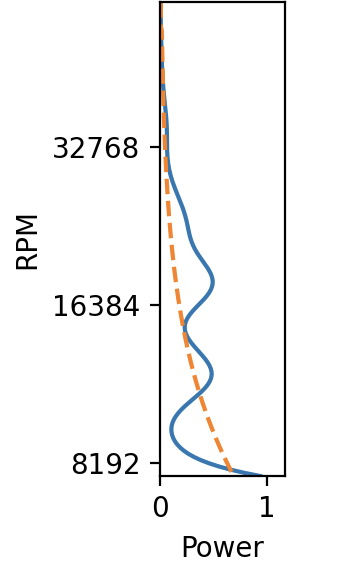
\includegraphics[width=0.25\linewidth]{Studienarbeit//images/cwt-red-noise.png}    
    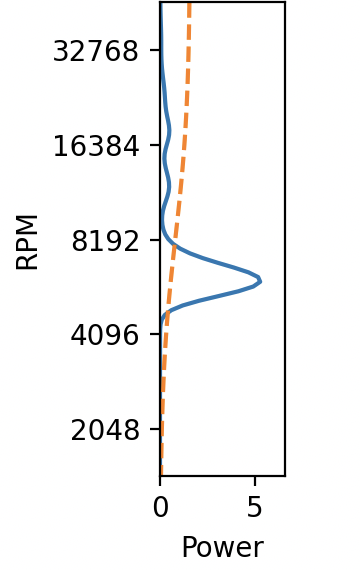
\includegraphics[width=0.25\linewidth]{Studienarbeit//images/cwt-inverse-red-noise.png}
    \caption{Anwendung verschiedener Filter auf das globale Wavelet-Spektrum}
    \label{fig:cwt-filter}
\end{figure}

Zu erkennen ist hierbei, dass durch den Red-Noise-Filter eher die tiefen Frequenzen isoliert werden und durch die inverse die hohen Frequenzen. 

\paragraph{Auswertung der Drehzahl}
Da durch den inversen Red-Noise-Filter vor allem die unteren Frequenzen isoliert werden wird klar, dass dieser Filter sich dazu eignet die Drehzahl zu bestimmen, da diese in diesem unteren Frequenzbereich liegt, wie an dem größten Peaks zu erkennen. Da für die Drehzahl die oberen Frequenzen keine Rolle spielen findet die weitere Verarbeitung mit diesem Filter statt. Wird nun ein Signifikanz-Test mit diesem Filter auf die Ergebnisse der \ac{CWT} angewendet, so entstehen die in der Abbildung \ref{fig:cwt-powerspek-1} gezeigten Plots. Die Beschriftung der Plots erfolgt ähnlich wie auch bei der \ac{STFT} mit der SOLL-RPM und SOLL-Schleifleistung. Die schwarzen Flächen sind jene Flächen, welche durch den Signifikanz-Test heraus gestochen sind, also nicht durch den Red-Noice-Filter ausgefiltert werden.

\begin{figure}[H]
    \centering
    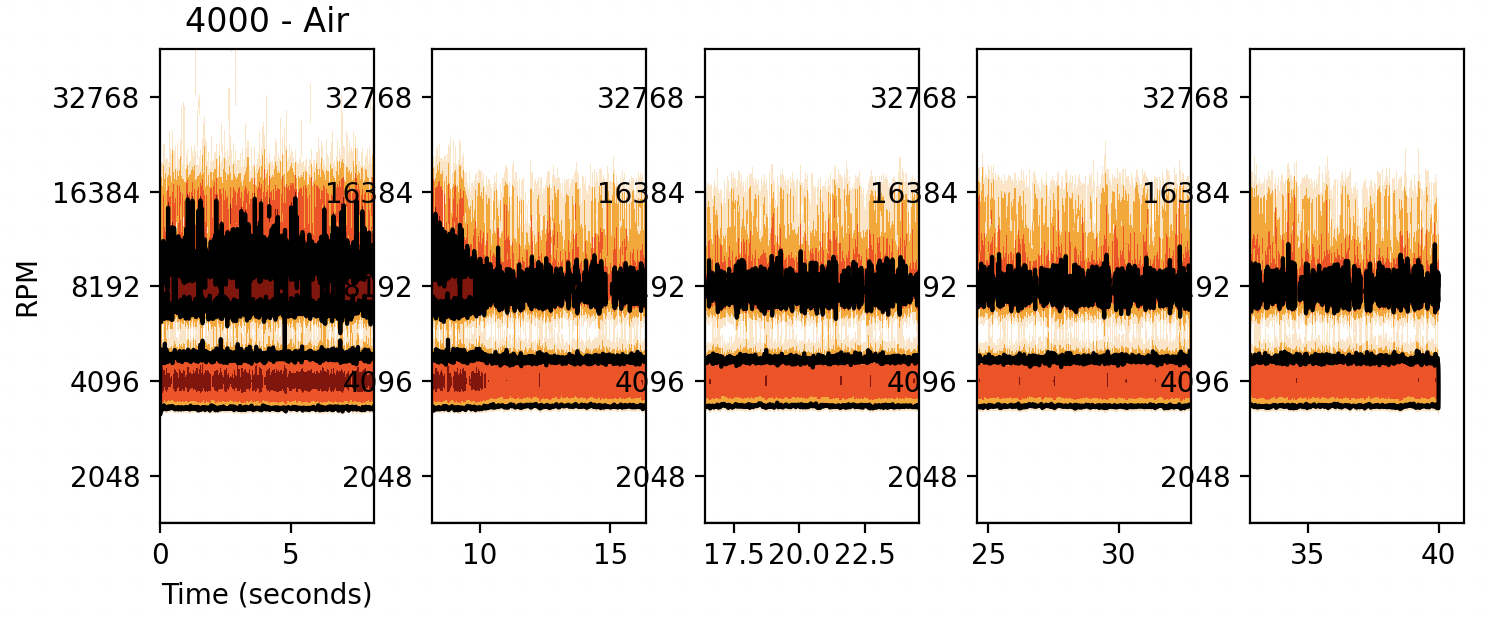
\includegraphics[width=0.8\linewidth]{Studienarbeit//images/cwt-4000-air.png}     
    \centering
    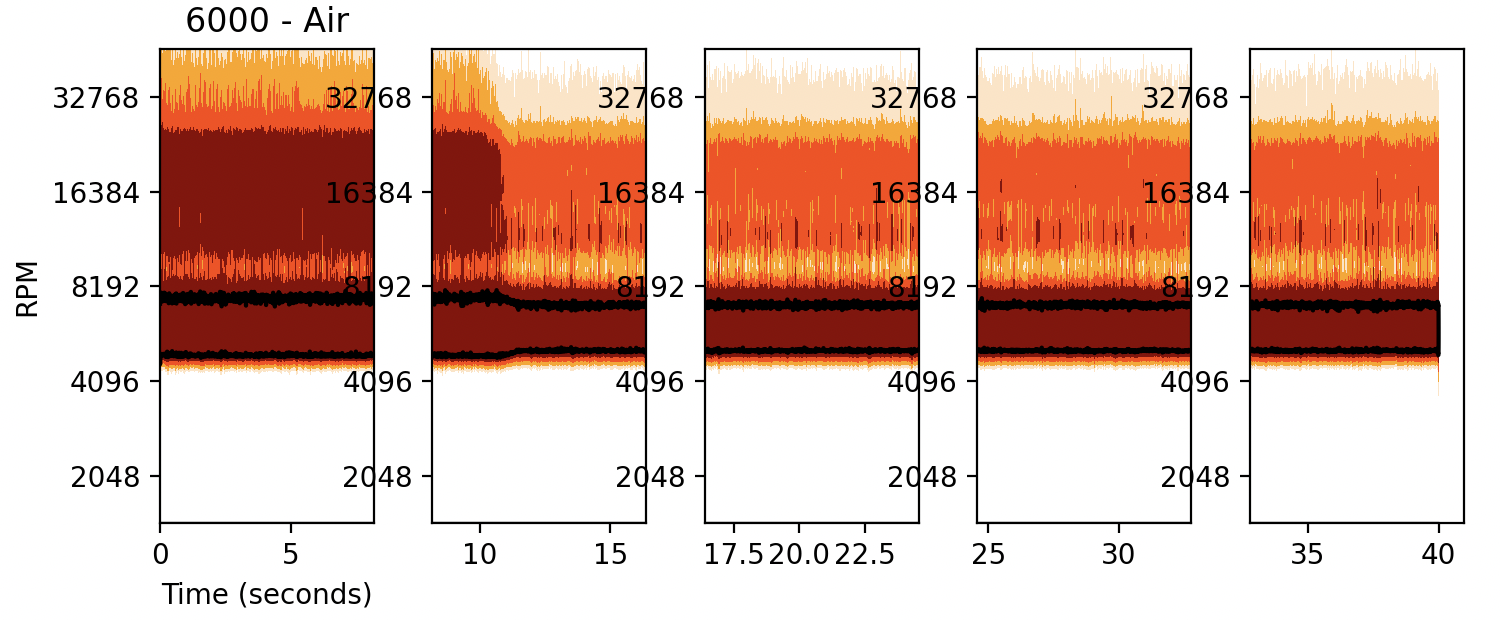
\includegraphics[width=0.8\linewidth]{Studienarbeit//images/cwt-6000-air.png}  
    \centering
    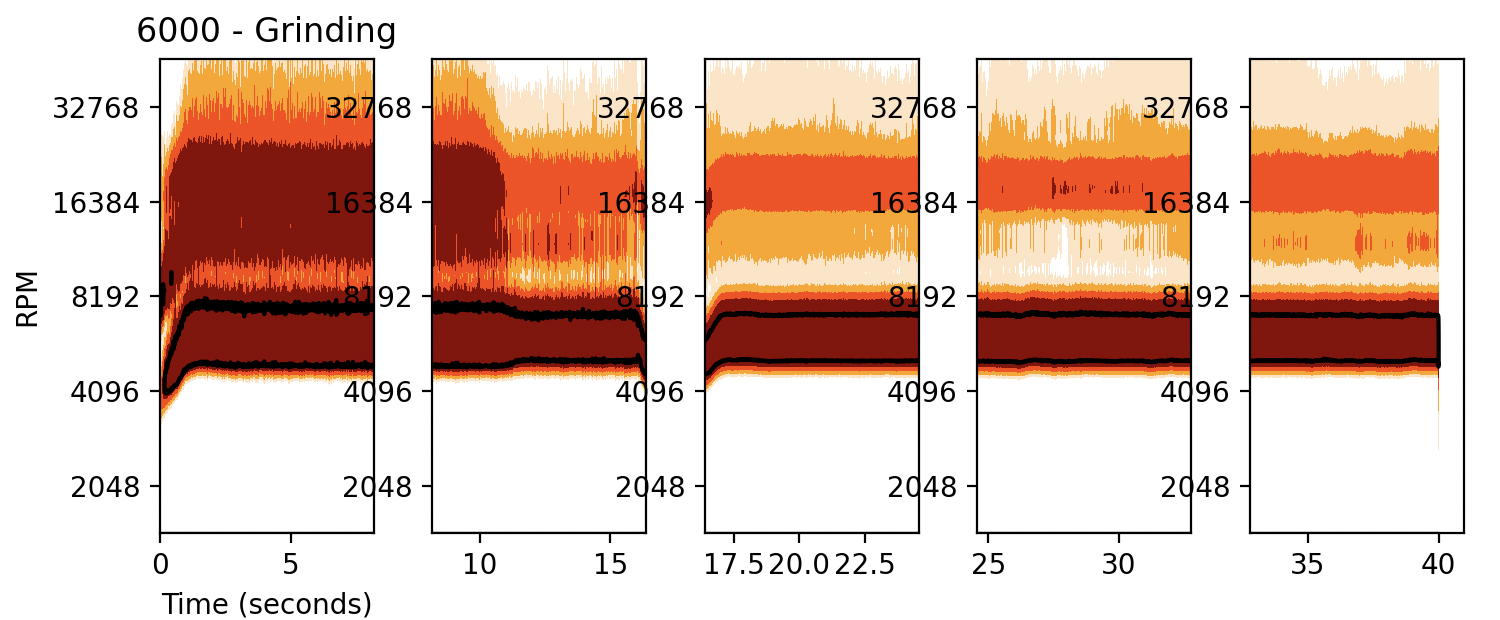
\includegraphics[width=0.8\linewidth]{Studienarbeit//images/cwt-6000-grinding.png}    
    \caption{Powerspektren verschiedener Audiosignale, als Ergebnis der CWT}
    \label{fig:cwt-powerspek-1}
\end{figure}


In der Abbildung deutlich zu erkennen ist, dass die höchsten Frequenzen sich im Bereich von 6000 RPM befinden. Zusätzlich wird deutlich, dass durch den Signifikanz-Test genau diese Frequenz nochmals isoliert wird und somit nur der Bereich um 6000 RPM eine hohe Signifikanz besitzt. Der Signifikante Bereich ist in der gezeigten Abbildung jeweils der, der sich zwischen den schwarzen Linien befinden. Vor allem interessant ist dies, da deutlich wird, dass dieser Bereich sowohl ohne erbrachte Schleifleistung (linkes Bild) als auch mit erbrachter Schleifleistung (rechtes Bild) gleich bleibt. Dies bildet nun den Vorteil gegenüber der \ac{STFT}, bei welcher die Frequenzen bei erbrachter Schleifleistung nicht mehr deutlich sichtbar waren. Durch diese Beobachtung lässt sich nun wiedereinmal eine Methode schreiben, welche immer die Frequenz eines bestimmten Zeitintervalls (z. B. einer Sekunde) ausliest, welche am stärksten ausgeprägt ist und sich gleichzeitig in durch den Signifikanz-Test heraus gestochenen Bereich befinden. So fließt in die Berechnung der höchsten Frequenz nicht nur die lokal stärkste Frequenz ein, sondern auch der globale Durchschnitt. Wendet man diese Methode nun an erhält man die in der Abbildung \ref{fig:cwt-rpm} gezeigten Plots. Auch hier wird nun wieder eine Intensität mit angegeben. Diese Intensität ist die aus der\ac{CWT} stammenden Intensität aber jedoch mit 1000 multipliziert, um die Visualisierung zu Verbessern. 

\begin{figure}[H]
    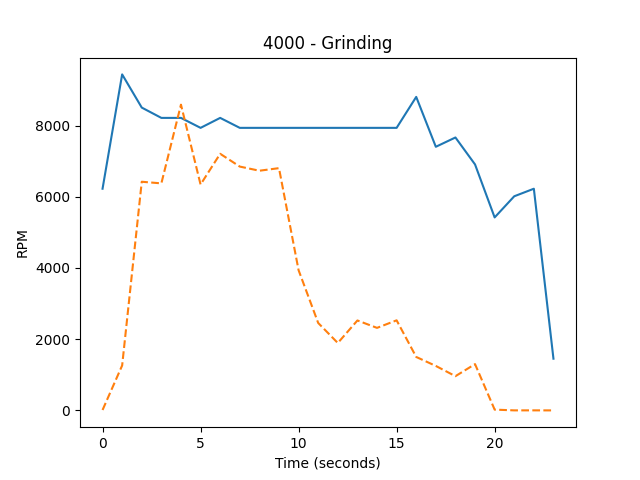
\includegraphics[width=0.5\linewidth]{Studienarbeit//images/cwt-rpm-4000-grinding.png} 
    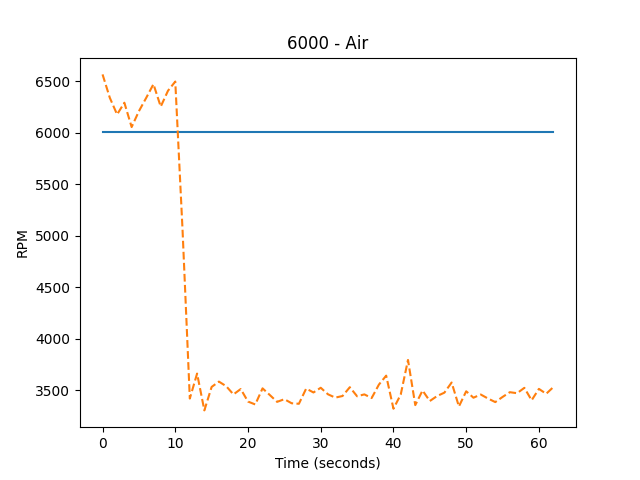
\includegraphics[width=0.5\linewidth]{Studienarbeit//images/cwt-rpm-6000-air.png}    
    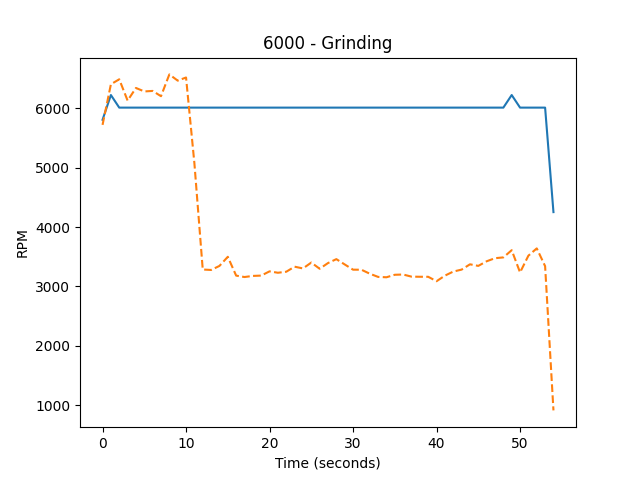
\includegraphics[width=0.5\linewidth]{Studienarbeit//images/cwt-rpm-6000-grinding.png}    
    \caption{Berechnung der Drehzahl auf Grundlage einer CWT}
    \label{fig:cwt-rpm}
\end{figure}


Betrachtet man sich nun diese Ergebnisse, fällt auf, dass die berechneten RPM bei 6000 RPM sehr genau sind und im Gegensatz zu der \ac{STFT} die Berechnung auch dann noch 6000 RPM ausgibt, wenn eine Schleifleistung erbracht wird, was bei der \ac{STFT} nicht der Fall war. Doch auch hier ist wiederum deutlich zu erkennen, dass bei den SOLL-4000 RPM als IST 8000 RPM ausgegeben werden. Dieses Ergebnis war jedoch zu erwarten, da wie bereits in der Abbildung \ref{fig:cwt-powerspek-1} zu erkennen ist, dass bei 4000RPM vor allem die doppelte Frequenz der Drehzahl über dem Signifikanz-Test liegt. Zwar könnte man hier eine Art Gaussian-Glocke über den Peak bei 8000 RPM legen, jedoch würde dies dann nur bei 4000RPM zu einem Ergebnis führen und bei allen anderen Drehzahlen wird das Ergebnis verschlechtert. Festhalten lässt sich an dieser Stelle, dass die Berechnung der Drehzahl auf Grundlage eines Signifikanz-Test auf einer\ac{CWT} hohe Erfolgschancen aufzeigt.


\paragraph{Auswertung von Schleifleistung}
Im letzten Abschnitt wurde die Methode beschrieben, mit welcher mithilfe der\ac{CWT} die RPM ausgerechnet werden können. Dieser Abschnitt richtet sich nun daran die dafür aufgetretenen Beobachtungen genauer zu betrachten und anhand-dessen einen Algorithmus zu finden, welcher den Schleif-Status innerhalb eines bestimmten Zeitintervalls berechnen kann. Wichtig an dieser Stelle zu erwähnen ist, dass die Beobachtungen nur um den Bereich von 6000 RPM gemacht werden konnten und sich dieser Abschnitt nur daran richtet die Schleifleistung um den Bereich von 6000 RPM bestimmen zu können. Betrachtet man sich nun noch einmal die Abbildung \ref{fig:cwt-powerspek-1}, so fällt auf, bei der dreifachen Frequenz des Schleifers häufig Anomalien auftreten, vor allem wenn das analysierte Audiosignal mit dem Label ,,Grinding'' versehen ist. Aus dieser Beobachtung lässt sich die Vermutung ableiten, dass diese Anomalie immer dann auftritt, wenn der Schleifer tatsächlich am Schleifen ist. Diese Vermutung gilt es nun zu überprüfen, indem diese Anomalie isoliert betrachtet wird. Um dies zu erreichen wird der Red-Noise-Filter verwendet, welcher die tieferen Frequenzen herausfiltert. Zusätzlich wird das Morlet-Wavelet so angepasst, dass nur die Frequenzen über 8000 RPM in der\ac{CWT} betrachtet werden. Die Auswahl des Filters und die Regelung dessen Stärke gelingt durch ausprobieren. Inwiefern der Filter angepasst werden muss, wurde durch die Anwendung des Filters auf das GWS verdeutlicht. Wird nun diese angepasste\ac{CWT} und der angepasst Filter des Signifikanz-Test angewendet, so erhält man die in der Abbildung \ref{fig:cwt-powerspek-2} gezeigten Power-Spektren. Rechts neben dem Power-Spektrum ist jeweils das GWS und der Filter zu sehen.

\begin{figure}[H]
    \centering
    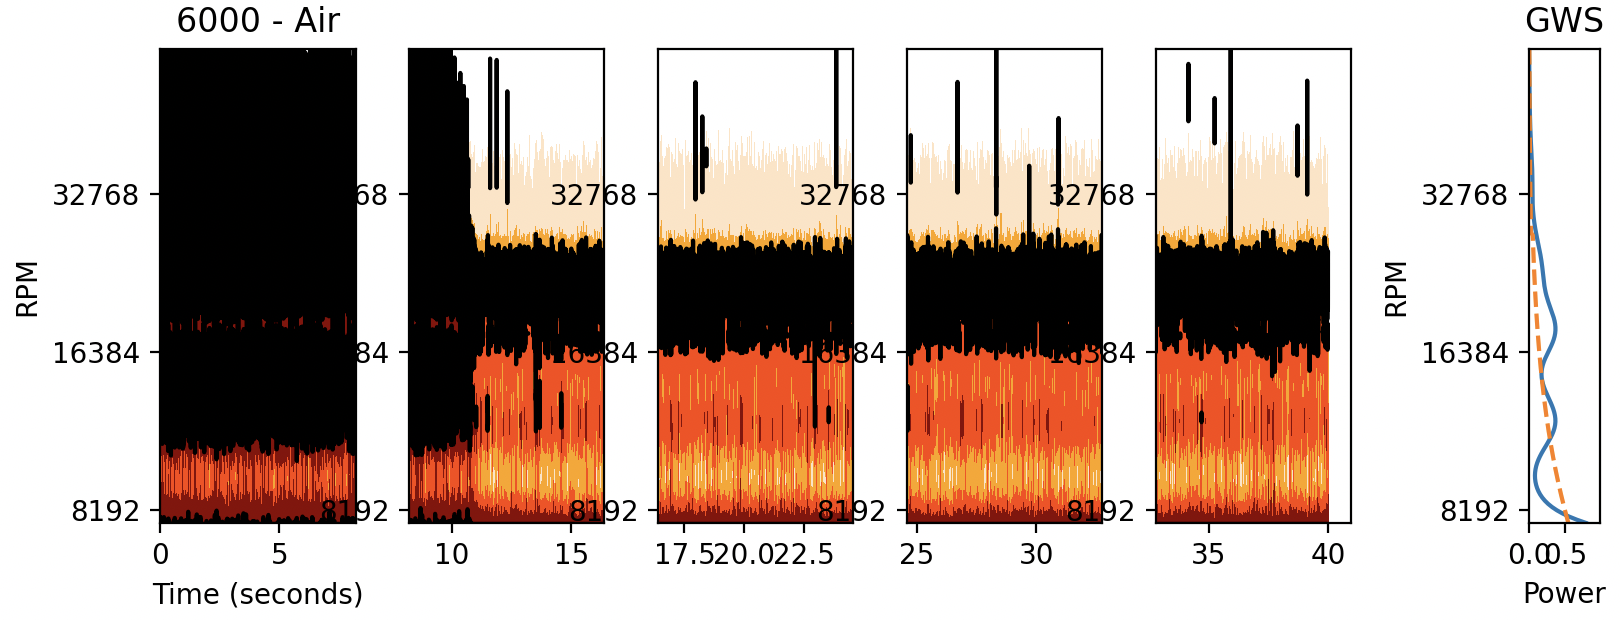
\includegraphics[width=0.8\linewidth]{Studienarbeit//images/cwt-iso-6000-air.png}    
    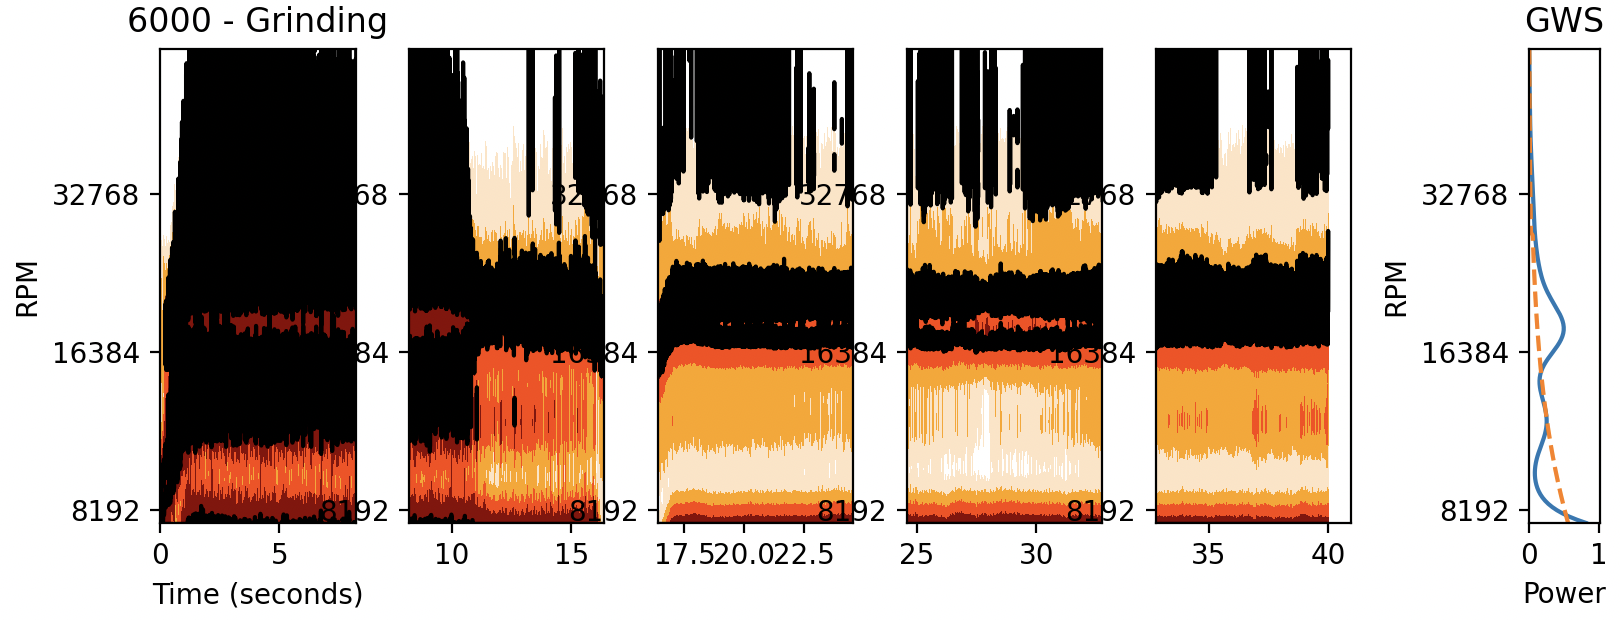
\includegraphics[width=0.8\linewidth]{Studienarbeit//images/cwt-iso-6000-grinding.png}   
    \caption{Powerspektrum isolierter Frequenzen, als Ergebnis der CWT}
    \label{fig:cwt-powerspek-2}
\end{figure}


Wie bereits im vorherigen Kapitel beschrieben markieren die schwarzen Flächen jeweils die Frequenzen, welche durch den Signifikanz-Test aufgefallen sind. Deutlich zu erkennen ist hier, dass der Signifikanz-Test in zwei Bereichen besonders ausschlägt. Bereich 1 ist der bereits vermutete Bereich bei der dreifachen Drehzahl des Schleifer und bei dem mit ,,Grinding'' markierten Datensätze schlägt der Signifikanz-Test auch ab dem Bereich von 32 000 vermehrt an.  Die Ausschläge über 32000 RPM entstehen vermutlich durch Rauschen, welches beim Schleifen des Werkstücks auftreten. Die Quelle dieses Rauschen ist leider unbekannt, womöglich stammt dies vom Material des Werkstücks oder der Schwingung des Werkstücks während des Schleifprozesses. Im nächsten Schritt werden nun diese auftretenden Bereiche genauer analysiert, um herauszufinden, welche Frequenz jeweils besonders heraus-sticht. Um nun die Daten Ergebnisse der\ac{CWT} genauer zu betrachten wird hier nun ähnlich wie auch zu Bestimmung der RPM eine Methode implementiert, welche immer jeweils immer die stärkste Frequenz im Zeitraum einer Sekunde bestimmt. Plottet man nun die Daten erhält man die in der Abbildung \ref{fig:cwt-iso-freqs} gezeigten Plots. 

\begin{figure}[H]
    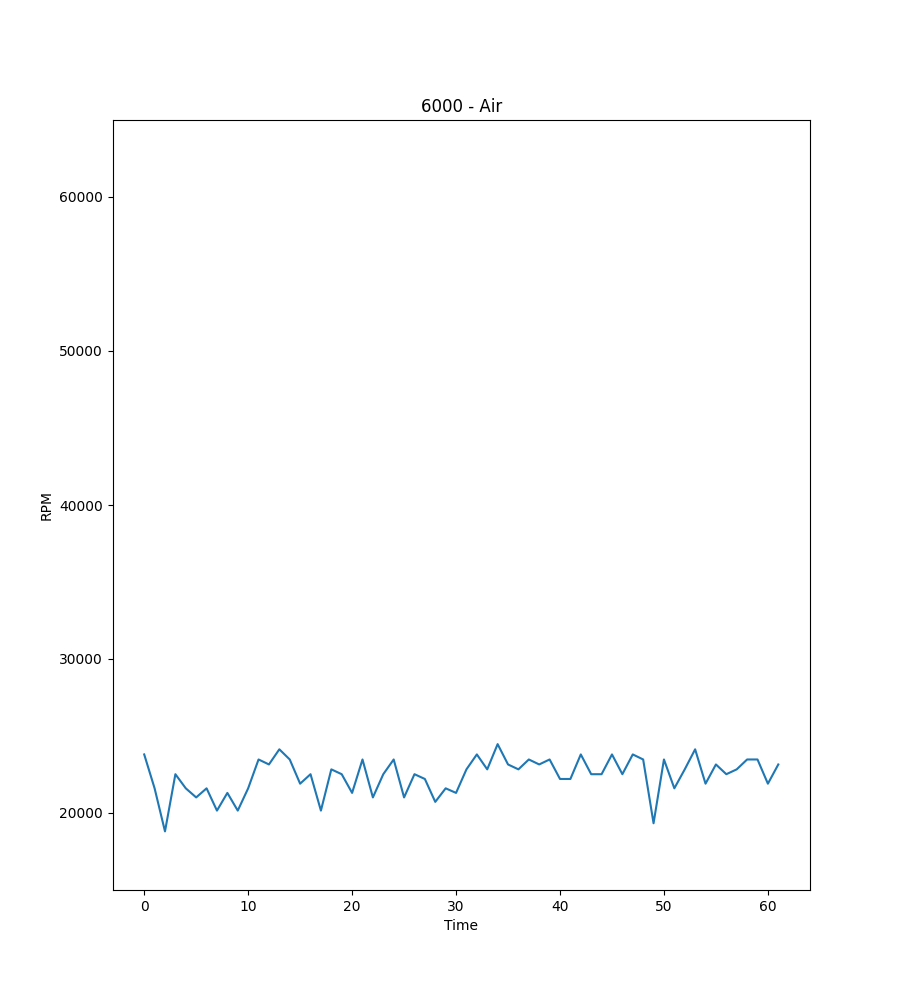
\includegraphics[width=0.5\linewidth]{Studienarbeit//images/cwt-6000-air-freqs-1.png}    
    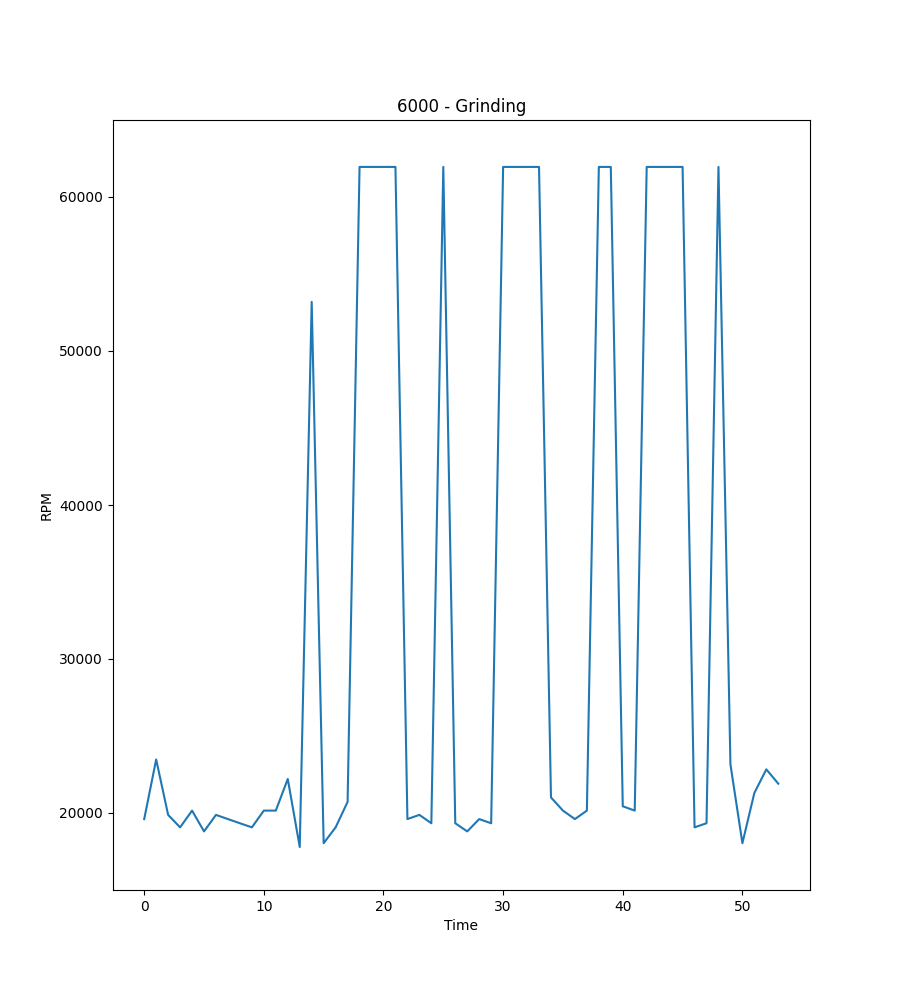
\includegraphics[width=0.5\linewidth]{Studienarbeit//images/cwt-6000-grinding-freqs-1.png}    
    \caption{Berechnung der am stärksten auftretenden Frequenz}
    \label{fig:cwt-iso-freqs}
\end{figure}

Hier zu erkennen ist deutlich, dass bei den Datensätzen, in welchem geschliffen wird tatsächlich viele Peaks im Bereich von 60000 RPM auftreten, welche der 10-fachen Drehzahl entsprechen, wobei erwähnt sein muss, dass es sich hierbei auch um Zufall handeln kann. Genauso wichtig zu erwähnen ist hierbei, dass die Quelle dieser Peaks unbekannt ist. So gibt es viele Faktoren, welche ein solches Rauschen verursachen können. Auch die Korrelation mit der Schleifleistung scheint hier zwar zu existieren, aber auch dabei kann es sich um Umstände handeln, die nur in genaue dieser exakten Umgebung des Roboters auftreten. Da diese Arbeit jedoch in erster Linie eine Machbarkeitsanalyse ist, die überprüft, ob überhaupt etwas aus den Daten heraus gelesen werden kann, wird an dieser Stelle mit diesen Daten weitergearbeitet und angenommen, dass die Frequenzen bei 60000 durch Schleifen erzeugt wird. Allen in allen wirken die Abbildungen recht ungenau und die gebildeten Platteua's bei 60000R RPM unnatürlich, weshalb sich im nächsten Schritt dafür entschieden wurde die Auflösung zu erhöhen. Dies wurde erreicht, indem das Zeitintervall, in welchem die stärkste Frequenz gesucht wird, verringert wird. Verschiedene dieser Zeitintervalle sind in der Abbildung \ref{fig:cwt-iso-freqs-genauigkeit} aufgezeigt. Grundlage für diese war immer das gleiche Audiosignal, um einen Vergleichswert zu schaffen.

\begin{figure}[H]
    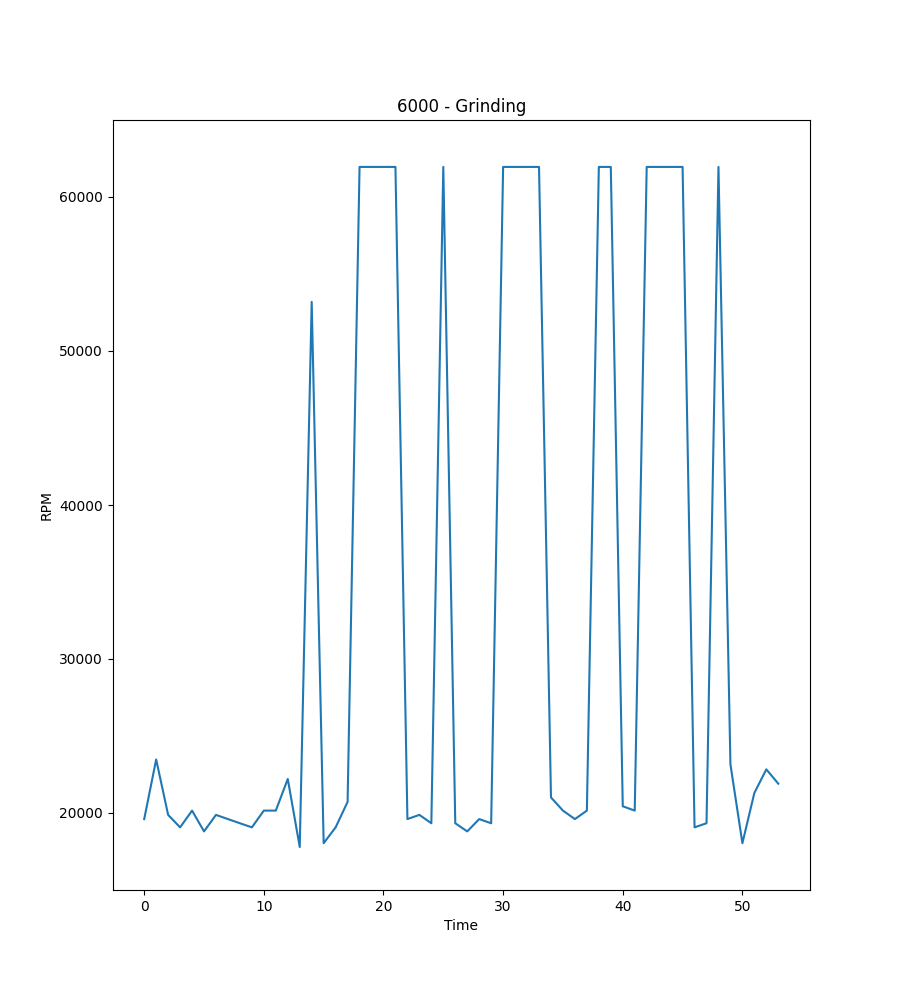
\includegraphics[width=0.5\linewidth]{Studienarbeit//images/cwt-6000-grinding-freqs-1.png} 
    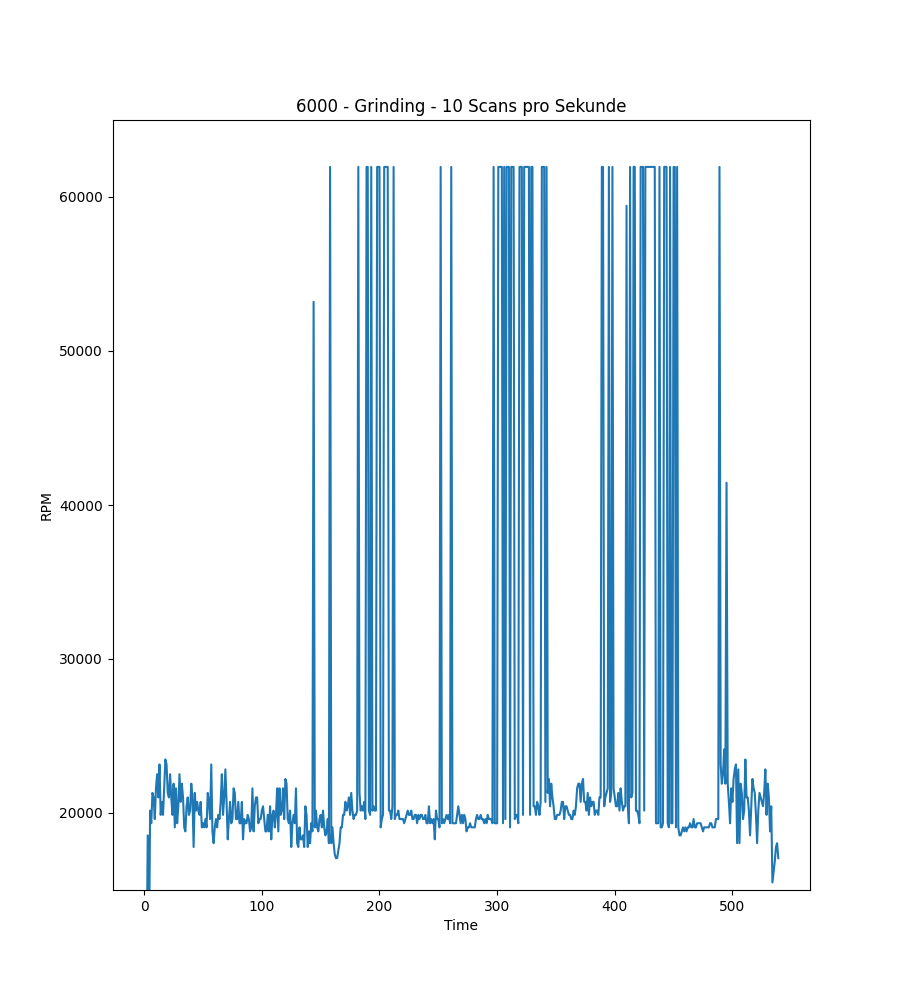
\includegraphics[width=0.5\linewidth]{Studienarbeit//images/cwt-6000-grinding-freqs-10.png}   
    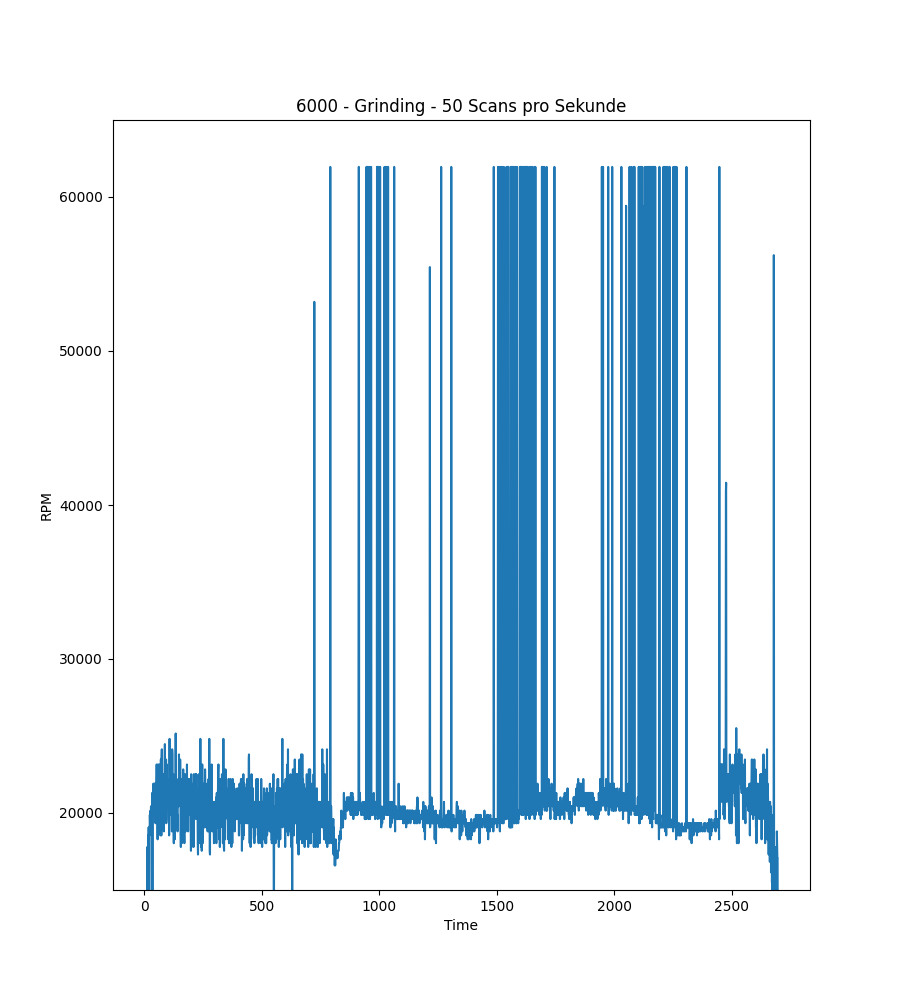
\includegraphics[width=0.5\linewidth]{Studienarbeit//images/cwt-6000-grinding-freqs-50.png}   
    \caption{Vergleich verschiedener zu untersuchende Zeitintervalle}
    \label{fig:cwt-iso-freqs-genauigkeit}
\end{figure}


Wie erwartet zeigt sich in höherer Auflösung, dass es sich bei den Plateaus, eigentlich nur um ganz viele Ganz kurze Peaks handelt. Dadurch wird klar, dass um die Schleifleistung zu bestimmen ein viel höherer Detaillierungsgrad notwendig ist, als zur Bestimmung der Drehzahl. Nun hat man   detaillierte Daten, welche Informationen über die Schleifleistung enthalten, diese müssen jetzt jedoch noch irgendwie richtig gedeutet werden. Eine Möglichkeit hierbei ist, sich den Mittelwert der Frequenzen innerhalb eines Zeitintervalls, z. B. einer Sekunde zu betrachten und mithilfe eines Grenzwertes festzulegen, ab welchem Mittelwert geschliffen wurde. Ein Mittelwert ist jedoch in der Hinsicht problematisch, dass die Frequenzen nicht bei 0 Anfangen und somit immer ein Bias existiert. Zwar könnte man auch in den Grenzwert mit einbeziehen, jedoch bietet die Stochastik genau dafür bereits eine Lösung an und zwar die Standardabweichung. Diese wird im nächsten Schritt berechnet, da diese selbst bei de gewählten Auflösung von 1/50s noch sehr kantig ist wird zusätzlich ein Mittelwert-Filter eingesetzt. Die Abbildung \ref{fig:cwt-std-mit-und-ohne-mittelwert-filter} zeigt nun diese Standardabweichung mit und ohne Mittelwert-Filter. 

\begin{figure}[H]
    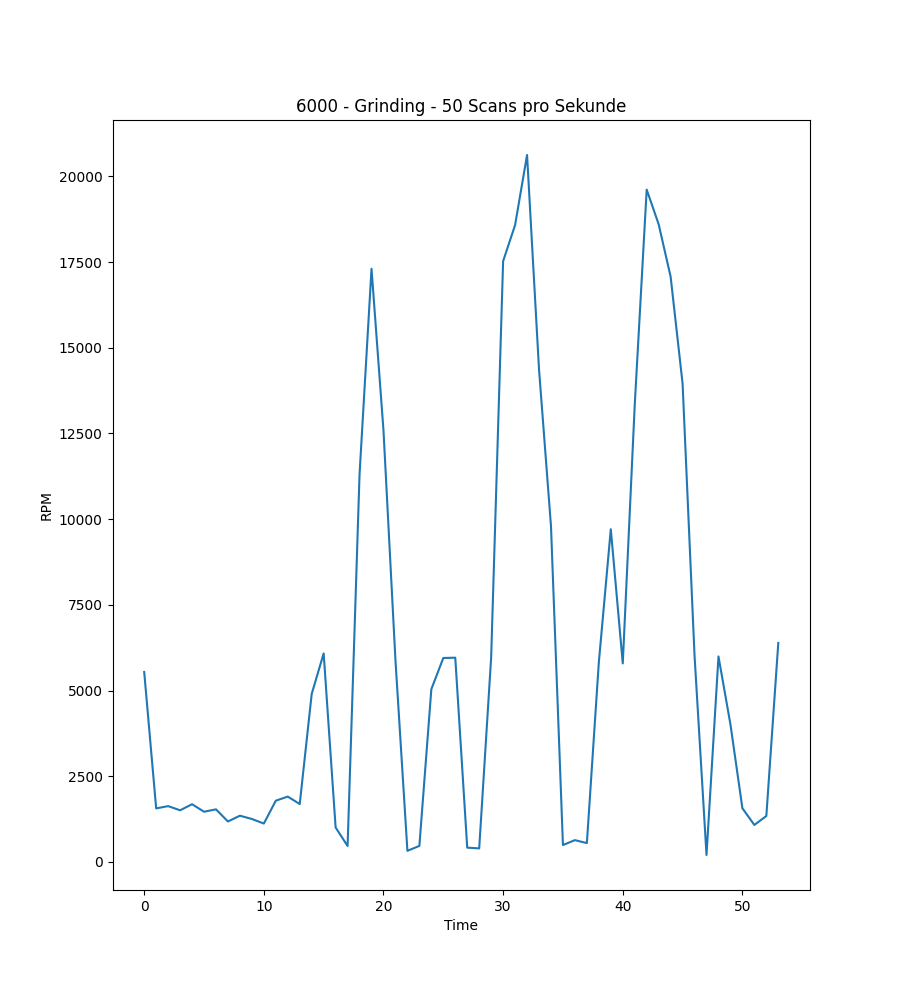
\includegraphics[width=0.5\linewidth]{Studienarbeit//images/cwt-6000-grinding-std.png} 
    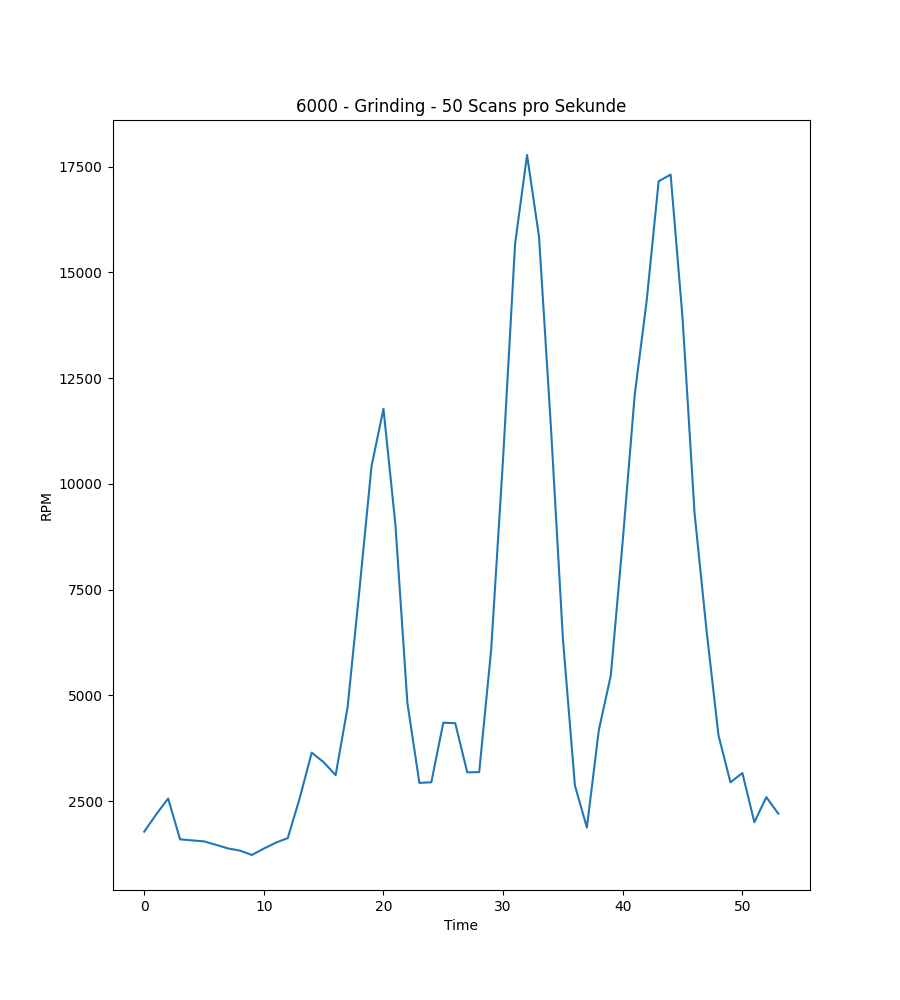
\includegraphics[width=0.5\linewidth]{Studienarbeit//images/cwt-6000-grinding-std-mw.png} 
    \caption{Standardabweichung mit und ohne Mittelwert-Filter}
    \label{fig:cwt-std-mit-und-ohne-mittelwert-filter}
\end{figure}

Da nun die Standardabweichung vorliegt muss ein Grenzwert festgelegt werden, aber welcher Standardabweichung ein Abschnitt als ,,Grinding'' eingeordnet hier. Durch die Auswertung mehrerer Datensätze fällt dieser Grenzwert auf 7500. Wichtig an dieser Stelle zu erwähnen ist, dass der Grenzwert vermutlich nur für eine Auswertung im Bereich von 6000 RPM gültig ist. Eine Berechnung dieses Grenzwertes ist an dieser Stelle leider nicht möglich, da es keine allgemeine Basis gibt, an welcher man sich orientieren kann. Zusätzlich kann sich der Grenzwert auch bei verschiedenen Materialien unterscheiden. Für den in Rahmen dieser Arbeit betrachte Schleifprozess ist dieser Grenzwert jedoch ausreichend und gibt sorgt für die grundlegende Erkenntnis darüber, dass eine akustische Vermessung eines robotischen Schleifprozesses funktionieren kann. Die Abbildung \ref{fig:cwt-schleif} zeigt nun das letztendliche Ergebnis mit einem von Grenzwert von 15000 auf verschiedene Audiosignale. Zur Veranschaulichung wurde ein Wert von 0 gewählt, wenn keine Schleifleistung erfolgt ist innerhalb der letzten Sekunde und ein Wert von 1 entspricht einer erbrachten Schleifleistung.

\begin{figure}[H]
    \centering
    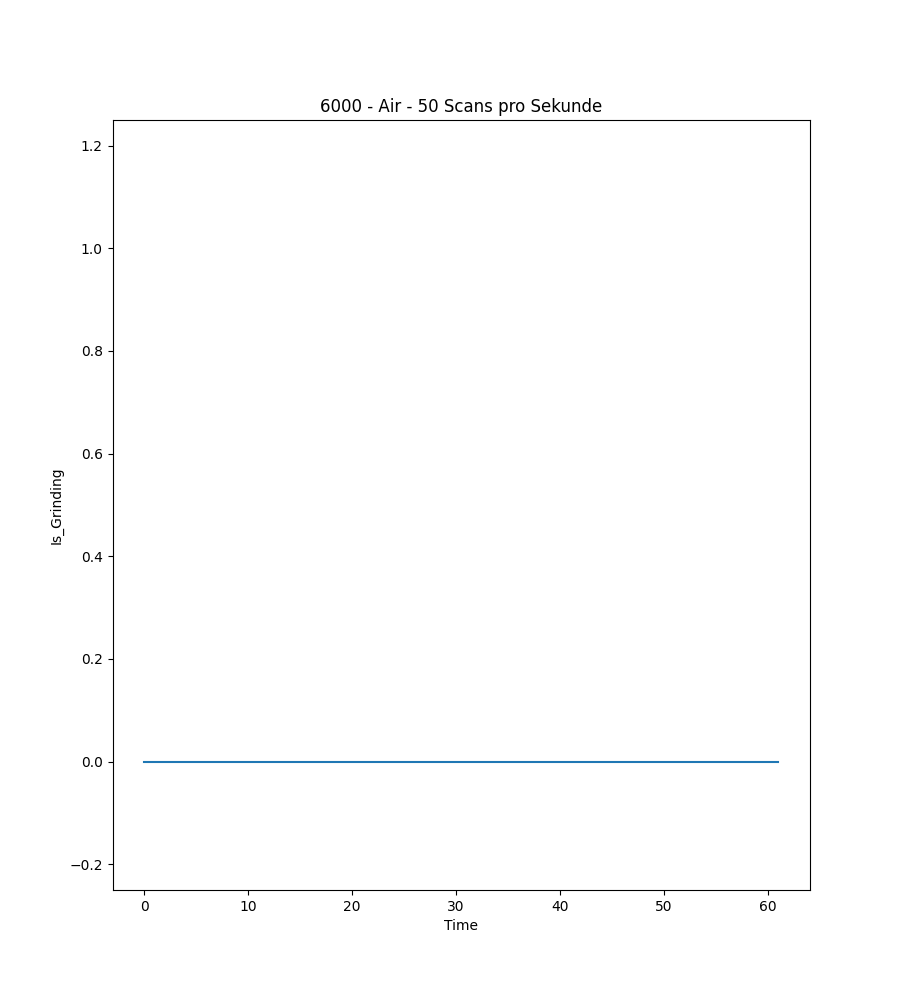
\includegraphics[width=0.44\linewidth]{Studienarbeit//images/cwt-6000-air-final-1.png} 
    \includegraphics[width=0.44\linewidth]{Studienarbeit//images/cwt-6000-grinding-final-2.png}

    \includegraphics[width=0.44\linewidth]{Studienarbeit//images/cwt-6000-grinding-final-3.png} 
    \includegraphics[width=0.44\linewidth]{Studienarbeit//images/cwt-6000-grinding-final-4.png} 
    \caption{Ergebnisse der Schleifleistung-Berechung}
    \label{fig:cwt-schleif}
\end{figure}

Die Ergebnisse zeigen deutlich, dass das Schleifgerät nicht zu jedem Zeitpunkt schleift. Auch bei den mit ,,Grinding'' markierten Audiosignalen kommt es so zu Zeitabschnitten, in welchen der Schleifer nicht schleift. Mithilfe einer solchen Darstellung kann nun analysiert werden, wie erfolgreich ein Schleifprozess war. Im folgenden Abschnitt werden nun die Ergebnisse dieser Durchführung nochmals zusammengefasst, zusätzlich werden Ideen für weitere Möglichkeiten erläutert, um diesen Prozess zu allgemeineren. Darin Anklang findet auch eine Klassifizierung mittels \ac{KI}, deren Umsetzbarkeit auch bereits im Kapitel \ref{Kapitel3} ausgiebig erläutert wurde.


\section{Ergebnis}
Im Letzten Kapitel wurden drei verschiedene Ansätze zur Audioanalyse getestet. Das Ziel war er herauszufinden, welche Informationen aus dem Audiosignal heraus gelesen werden können. Der erste Ansatz, welcher hier benutzt wurde war die \ac{FFT}, also eine Fourier-Transformationen. Diese ist bildete viele Jahre lang die Grundlage für jegliche Signalanalyse, so auch in diesem Anwendungsfall. Die Betrachtung der Audiosignale im Frequenzraum hat dazu geführt, dass sichtbar wurde, dass zum einen die Drehzahl des Schleifers zu erkennen ist, als auch ein Rauschen in den Audiosignalen, in denen geschliffen wurde. Nun ist jedoch auch der Fall, dass sichtbar wurde, dass bei einem SOLL von 4000RPM die stärkste Frequenz auf ein IST von 8000RPM hingedeutet hat. Dieses Problem ist vermutlich auf eine Eigenschwingung des Motors zurückzuführen, welche bei 4000RPM verstärkt wird. Diese Erkenntnis hat dann dazu beigetragen, dass sich in den Folgenden Ansätzen und bei der Analyse der Schleifleistung auf ein SOLL von 4000RPM beschränkt wurde. Letztendlich reichte die \ac{FFT} jedoch nicht aus um detaillierte Informationen sinnvoll auszulesen, weshalb sich dazu entschieden wurde der zeitlichen Komponente mehr Bedeutung zu geben. Hierfür wurde eine \ac{STFT} implementiert. Die Ergebnisse dieser \ac{STFT} bestätigten nochmals die Anomalie bei 4000RPM und bestätige auch, dass die Drehzahl bei SOLL 6000RPM abgelesen werden kann. Zudem wurden durch die zeitliche Komponente weitere Anomalien in den Ergebnissen sichtbar. Eine Anomalie lies auf ein Rauschen in den ersten 10 Sekunden jedes Audiosignals deuten, die andere Anomalie zeigt, dass allgemein viel mehr Rauschen in den Audiosignalen vorhanden ist, in welchen wahrscheinlich geschliffen wurde. Da jedoch auch diese Ergebnisse nicht sehr detailliert waren und zudem stark abhängig von den gewählten Parametern der STFT, kam schließlich eine\ac{CWT} zum Einsatz. Die Durchführung dieser verdeutlichte die davor aufgestellten Vermutungen und zeigte deutlich, dass die Berechnung der Drehzahl funktioniert. Zusätzlich offenbarte die\ac{CWT} auch, dass die Schleifleistung sich offenbar mit der dreifachen Frequenz korreliert, aus diesem Grund wurde die\ac{CWT} dann so verfeinert, dass dieser Frequenzbereich isoliert wurde. Die Auswertung zeigte dann jedoch, dass zwar auch die dreifache Drehzahl irgendwie mit der Schleifleistung zusammenhängt, viel auffälliger war hier jedoch ein Rauschen, welches sich im Bereich vom 5-10 fachen Drehzahlbereich befindet. Beim Auslesen der stärksten Frequenzen zeigte sich dann, dass im Falle einer erbrachten Schleifleistung zwischen der dreifachen-Drehzahl und der zehnfachen Drehzahl hin und her springen, während in Audiosignalen ohne Schleifleistung diese stärkste Frequenz konstant bei der dreifachen Drehzahl lag. Dies ermöglichte es dann anhand der Standardabweichung, der stärksten Drehzahl innerhalb eines Zeitintervalls, zu bestimmen, ob in diesem Zeitintervall geschliffen wurde oder nicht. Hierfür wurde ein fester Grenzwert festgesetzt. Soviel zu den erzielten Ergebnissen, nun folgt eine Bewertung dieser Ergebnisse. 

Auf den ersten Blick scheinen die Ergebnisse sehr gut zu sein, jedoch müssen hierbei einige Dinge beachtet werden. Erst einmal wurden alle Audiosignale in einer geschlossenen Atmosphäre aufgenommen, wobei immer das gleiche Material geschliffen wurde. Zusätzlich ist es möglich, dass gewisse Anomalien gar nicht durch das Schleifen selbst, sondern durch beispielsweise die Befestigung des Materials entstand. So ist es möglich, dass diese gefundene Anomalie bei der 10-fachen Drehzahl also nicht auf das Schleifen zurückzuführen ist und nur in genau dieser Prototypischen Umgebung existiert, in der geschliffen wurde. Dies führt zeitgleich auch dazu, dass dieser festgelegte Grenzwert möglicherweise nur in dieser Umgebung gute Ergebnisse liefert. Auch wichtig anzumerken ist, dass es nur möglich war diese Erkenntnisse bei Audiosignalen zu treffen, welche im Bereich von 6000 RPM aufgenommen wurde. Bei 4000 RPM trat Rauschen auf, welches es nicht ermöglichte automatische Analysen zu machen. Insgesamt lässt sich hier also festhalten, dass die erzielten Ergebnisse mit Vorsicht zu betrachten sind und die Methoden zur Analyse der RPM und der Schleifleistung nur in diesem prototypischen Umfeld gute Ergebnisse erzielen kann.

Insgesamt zeigen aber genau diese Ergebnisse, dass es möglich ist Methoden zu entwickeln, welche eine prädiktive Wartung ermöglichen. Aus diesem Grund haben wir uns auch dafür entschieden in Kapitel \ref{Kapitel3} mögliche State of the Art Lösungen zum Thema KI zu betrachten. Die verschiedenen Ergebnisse zeigen deutlich, dass Muster in den Daten zu erkennen sind. Diese Muster gilt es nur auszulesen. Dies ist mit ,,einfachen'' Algorithmen nicht gelungen, doch der Einsatz von KI scheint hier erfolgversprechend zu sein, da wie bereits erwähnt ähnliche Klassifizierungen und Analysen in diesem Bereich bereits mit Erfolg in diesem Bereich durchgeführt wurden. Klar stellt sich nun die Frage, wieso diese Arbeit die Analyse mit KI nicht in Betracht gezogen hat. Der Grund dafür liegt darin, dass die Datengrundlage viel zu gering ist, um eine KI von neu auf zu trainieren. So wäre es notwendig gewesen mehrere Tausende Daten manuell aufzunehmen und zu Labeln, wobei nicht mal sichergestellt ist, dass die Label richtig sind. Aus diesem Grund lag die Entscheidung nahe, dass es erst mal wichtig ist grundsätzlich die Daten zu analysieren, um aufzuklären, ob überhaupt Muster in den Daten zu erkennen sind, die dann von einer KI analysiert werden können. Zusätzlich zeigt diese Arbeit auch Möglichkeiten zur Vorverarbeitung von Daten und ermöglicht es zugleich, dass nicht alle Daten manuell gelabelt werden müssen, sondern der aufgezeigte Algorithmus dieses Labeln übernehmen kann. Manuell müssen diese Labels dann nur noch stichprobenartig überprüft werden. Insgesamt zeigt diese Arbeit also auf, dass sehr wohl die grundsätzliche Möglichkeit besteht, Eigenschaften über den Schleifprozess aus den Audiosignalen aus.


%%%%%%%%%%%%%%%%%%%%%%%%%%%%%%%%%%%%%%%%%%%%%%%%%%%%%%%%%%%%%%%%%%%%%%%%%%%%%%%
\endinput
%%%%%%%%%%%%%%%%%%%%%%%%%%%%%%%%%%%%%%%%%%%%%%%%%%%%%%%%%%%%%%%%%%%%%%%%%%%%%%%

\chapter{ROS-Node zur Analyse der Signale}
\label{Kapitel7}

Um nun die Algorithmen zum Auswerten der Audio-Signale über ROS zur Verfügung zu stellen wird in diesem Kapitel zu Erstellung einer ROS-Node beschrieben, welche die notwendigen Daten publisht. Die Anforderungen an diese Node sind, dass man im Vorhinein einen Pfad angibt, unter welchem das zu analysierende Audiosignal jeweils verfügbar ist. Des Weiteren müssen die Audiosignale länger als eine Sekunde sein, da die Genauigkeit der Ausgabe auf Sekundenebene ist.

Um nun die ROS-Node zu erzeugen wird eine Python-Methode erstellt. Der erste Schritt darin ist über die Python-Bibilothek rospy eine Node zu initialisieren. In unserem Fall erhält die Node den Namen ,,\texttt{grinding\_audio\_data\_publisher}''. Da die Node nur Daten publishen soll, wird im nächsten Schritt ein Publisher erzeugt, auch über rospy. Dieser Publisher ist das Topic, unter dem gepublished wird, mit dem Namen ,,\texttt{grinding\_data}'', zusätzlich wird hier festgelegt, dass die Nachrichten als \texttt{String} gepublished werden. Nachdem nun die Node und das Topic erstellt wurden, werden die Daten analysiert, indem das Audiosignal, zu welchem der hart-codierte Pfad führt, ausgelesen und anschließend verarbeitet wird. Für die Analyse werden getrennt die zwei Algorithmen aufgerufen, welche im letzten Kapitel beschrieben wurden. Algorithmus 1 berechnet die RPMs und deren Intensität, Algorithmus 2 berechnet die Grinding-Stati.Diese Daten werden anschließend über eine for-Schleife gepublished. Hierbei werden immer die Daten für eine Sekunde als String ausgegeben. Das Publishen erfolgt mit einer Frequenz von 10Hz.


%%%%%%%%%%%%%%%%%%%%%%%%%%%%%%%%%%%%%%%%%%%%%%%%%%%%%%%%%%%%%%%%%%%%%%%%%%%%%%%
\endinput
%%%%%%%%%%%%%%%%%%%%%%%%%%%%%%%%%%%%%%%%%%%%%%%%%%%%%%%%%%%%%%%%%%%%%%%%%%%%%%%
\part{Fazit und Ausblick}
\chapter{Fazit}
\label{Kapitel8}

In dieser Arbeit wurde ein umfassender Ansatz zur Analyse von Audiosignalen im Kontext eines robotischen Schleifprozesses entwickelt und evaluiert. Die Hauptziele bestanden darin, Frequenzmuster zu erkennen, die mit der Drehgeschwindigkeit des Schleifers und dem Anpressdruck korrelieren, sowie die Machbarkeit einer akustischen Überwachung zur prädiktiven Wartung zu prüfen. Hierzu wurden verschiedene Methoden der Signalverarbeitung angewendet und verglichen. In diesem Kapitel werden nun die Ergebnisse nochmal kurz zusammengefasst und kritisch refektiert.

\section{Zusammenfassung der Hauptergebnisse}
\subsection{Datenaufnahme}

Bei der Datenaufnahme wurden zwei Methoden untersucht: automatisches und manuelles Schleifen. Das automatische Schleifen durch vorprogrammierte Bahnen erwies sich als problematisch, da der konstante Anpressdruck bei schrägen Werkstücken dazu führte, dass der Schleifer kippte. Beim manuellen Schleifen war es schwierig, konsistent zu arbeiten, weil die Steuerung komplizierter ist und der Anpressdruck zu Beginn oft zu hoch war, was zu einer ungleichmäßigen Druckverteilung über das Schleifstück führte. Zudem gab es anfänglich Probleme mit der Befestigung des Mikrofons, das sich durch die Vibrationen des Roboters während des Schleifens absenkte und die Distanz zum Schleifer veränderte. Dieses Problem wurde durch erneutes Festziehen der Schrauben behoben.

\subsection{Ergebnisse der Datenanalyse}

Zur Analyse der Schleifgeräusche wurden drei verschiedene Audioanalysemethoden getestet: Die Fast Fourier Transformation, die Short-Time Fourier Transformation und die Continuous Wavelet Transformation.

\begin{itemize}
    \item \textbf{\ac{FFT}}:
        Die \ac{FFT} zeigte auf, dass in den Audiodaten Informationen enthalten sind, welche sich möglicherweise auf die verwendete Drehzahl und die Schleifleistung zurückführen lassen. Auffällig an dieser Stelle war eine Anomalie bei einer SOLL-Drehzahl von 4000 RPM, da hier die doppelte Frequenz und nicht die einfache Frequenz besonders stark ausgeprägt war.
    \item \textbf{\ac{STFT}}:
        Die \ac{STFT} lieferte weitere detaillierte Informationen, vor allem über die zeitliche Komponente. Auch hier war die Anomalie bei einer SOLL-Drehzahl noch deutlich zu erkennen, was zu der Annahme führte, dass es sich hierbei um ein Rauschen handelt, welches nicht verhindert werden kann, da es sich über das gesamte Audiosignal ausbreitet. Auf grundlage der STFT konnte eine erste Methode zur Berechnung der IST-Drehzahl implementiert werden, welche jedoch sehr fehleranfällig war. Da die Ergebnisse bei der \ac{STFT} stark von den gewählten Parametern abhängig sind, kam die Vermutung auf, dass die Ergebnisse durch eine \ac{CWT} besser sind.

    \item \textbf{\ac{CWT}}:
        Die \ac{CWT} bestätigte nun alle vorherigen Vermutungen und hat bewiesen, dass eine Berechnung der IST-Drehzahl bei 6000 RPM mit hoher Wahrscheinlichkeit gelingen kann. Eine Auswertung von anderen IST-Drehzahlen blieb weiterhin sehr ungenau. Zusätzlich zeigte sich durch die CWT eine Korrelation der Schleifleistung und der dreifachen Frequenz der Drehzahl. Als diese Frequenz dann isoliert betrachtet wurde zeigte sich, dass ein auffälliges Rauschen im Bereich des 5-10-fachen der Drehzahl während des Schleifprozesses auftritt. Durch die Analyse der genauen Existenz dieses Rauschen konnte dann eine Methode entwickelt werden, die Anhand der Standardabweichung der stärksten Drehzahl innerhalb eines Zeitintervalls bestimmt, ob in diesem Intervall geschliffen wurde oder nicht. Hierbei diente ein fester Grenzwert  als Entscheidungskriterium.
\end{itemize}


\section{Kritische Reflexion}

Auf den ersten Blick scheinen die Ergebnisse sehr gut zu sein, jedoch müssen hierbei einige Dinge beachtet werden. Erstens wurden alle Audiosignale in einer geschlossenen Atmosphäre aufgenommen, wobei immer das gleiche Material geschliffen wurde. Dies stellt eine kontrollierte, aber auch stark eingeschränkte Umgebung dar. 

Zusätzlich ist es möglich, dass gewisse Anomalien nicht durch das Schleifen selbst, sondern durch die Befestigung des Materials entstanden sind. Beispielsweise könnte die gefundene Anomalie bei der 10-fachen Drehzahl nicht auf das Schleifen zurückzuführen sein und nur in dieser prototypischen Umgebung existieren. Dies führt dazu, dass der festgelegte Grenzwert möglicherweise nur in dieser Umgebung gute Ergebnisse liefert. 

Ein weiterer kritischer Punkt ist, dass die Erkenntnisse nur bei Audiosignalen getroffen werden konnten, die im Bereich von 6000 RPM aufgenommen wurden. Bei 4000 RPM trat ein Rauschen auf, welches automatische Analysen verhinderte. Insgesamt lässt sich festhalten, dass die erzielten Ergebnisse mit Vorsicht zu betrachten sind und die Methoden zur Analyse der RPM und der Schleifleistung nur in diesem prototypischen Umfeld zuverlässige Ergebnisse liefern können.

Insgesamt können die kritschen Punkte wie folgt zusammengefasst werden.
\begin{itemize}
    \item \textbf{Einfluss externer Faktoren}: Die Ergebnisse könnten durch externe Faktoren wie Temperaturschwankungen, Luftfeuchtigkeit oder andere Umgebungsbedingungen beeinflusst werden, die in der kontrollierten Umgebung konstant gehalten wurden. Diese Faktoren könnten in einer realen Anwendung variieren und die Ergebnisse verfälschen.
    \item \textbf{Materialvariationen}: Die Analyse wurde nur mit einem einzigen Materialtyp durchgeführt. Unterschiede in der Materialhärte, Oberflächenbeschaffenheit oder Zusammensetzung könnten die Schleifgeräusche und damit die Analyseergebnisse erheblich beeinflussen.
    \item \textbf{Langzeitstabilität}: Es bleibt unklar, wie stabil die Ergebnisse über längere Zeiträume sind. Verschleiß am Schleifer, Veränderungen an den Befestigungen oder andere altersbedingte Faktoren könnten die Zuverlässigkeit der Analyse beeinträchtigen.
    \item \textbf{Granularität der Daten}: Die Analyse könnte durch die Auflösung der Audiodaten oder die Samplingrate der Aufnahmen beeinflusst werden. Höhere Granularität könnte zu detaillierteren, aber auch zu komplexeren Daten führen, die schwerer zu analysieren sind.
\end{itemize}

Insgesamt zeigen aber genau diese Ergebnisse, dass es möglich ist, Methoden zu entwickeln, welche eine prädiktive Wartung ermöglichen. Aus diesem Grund haben wir uns auch dafür entschieden, in Kapitel \ref{Kapitel3} mögliche State-of-the-Art-Lösungen zum Thema Künstliche Intelligenz (KI) zu betrachten. Die erzielten Ergebnisse zeigen deutlich, dass Muster in den Daten zu erkennen sind. Diese Muster gilt es nur auszulesen. Dies ist mit ''einfachen'' Algorithmen nicht gelungen, doch der Einsatz von KI scheint hier erfolgversprechend zu sein, da ähnliche Klassifizierungen und Analysen bereits mit Erfolg durchgeführt wurden.

Die Frage, warum diese Arbeit die Analyse mit KI nicht in Betracht gezogen hat, lässt sich durch die unzureichende Datengrundlage erklären. Um eine KI von Grund auf zu trainieren, wäre es notwendig gewesen, mehrere Tausend Daten manuell aufzunehmen und zu labeln, wobei nicht einmal sichergestellt ist, dass die Labels korrekt sind. Daher war es wichtig, zunächst die Daten zu analysieren, um festzustellen, ob überhaupt Muster vorhanden sind, die dann von einer KI analysiert werden könnten.

Zusätzlich zeigt diese Arbeit Möglichkeiten zur Vorverarbeitung von Daten und ermöglicht es, dass nicht alle Daten manuell gelabelt werden müssen. Der aufgezeigte Algorithmus kann dieses Labeln übernehmen, und die Labels müssen dann nur noch stichprobenartig überprüft werden. Insgesamt zeigt diese Arbeit, dass die grundsätzliche Möglichkeit besteht, Eigenschaften des Schleifprozesses aus den Audiosignalen zu extrahieren.

    
%%%%%%%%%%%%%%%%%%%%%%%%%%%%%%%%%%%%%%%%%%%%%%%%%%%%%%%%%%%%%%%%%%%%%%%%%%%%%%%
\endinput
%%%%%%%%%%%%%%%%%%%%%%%%%%%%%%%%%%%%%%%%%%%%%%%%%%%%%%%%%%%%%%%%%%%%%%%%%%%%%%%
\chapter{Ausblick}
\label{Kapitel9}

Die vorliegenden Ergebnisse und deren kritische Betrachtung legen nahe, dass es mehrere vielversprechende Forschungsrichtungen gibt, um die prädiktive Wartung weiter voranzutreiben. Diese Themen könnten in zukünftigen Arbeiten vertieft werden:

\paragraph{Erweiterung der Datengrundlage}

Um die Robustheit und Generalisierbarkeit der Analyseverfahren zu verbessern, könnten zukünftige Studien eine umfangreichere Datengrundlage schaffen. Dies beinhaltet:
\begin{itemize}
    \item \textbf{Unterschiedliche Materialien}: Die Aufnahme und Analyse von Audiosignalen bei verschiedenen Materialtypen würde helfen, die Algorithmen auf eine breitere Anwendungsbasis zu erweitern.
    \item \textbf{Verschiedene Umgebungsbedingungen}: Datenaufnahmen unter variierenden Umweltbedingungen wie Temperatur, Luftfeuchtigkeit und Umgebungsgeräuschen könnten die Robustheit der Analyse verbessern.
    \item \textbf{Langzeitstudien}: Langfristige Beobachtungen und Datenaufnahmen könnten helfen, die Stabilität und Zuverlässigkeit der Analyse über längere Zeiträume zu gewährleisten.
\end{itemize}

\paragraph{Verbesserung der Analysemethoden}

Die verwendeten Audioanalysemethoden könnten durch fortschrittlichere Techniken ergänzt oder ersetzt werden:
\begin{itemize}
    \item \textbf{Künstliche Intelligenz und Maschinelles Lernen}: Der Einsatz von KI und maschinellem Lernen, insbesondere Deep Learning, könnte die Erkennung und Analyse komplexer Muster in den Audiodaten verbessern. Eine größere und vielfältigere Datengrundlage würde es ermöglichen, Modelle zu trainieren, die verlässliche Vorhersagen treffen können.
    \item \textbf{Hybride Modelle}: Eine Kombination aus traditionellen Signalverarbeitungstechniken und modernen KI-Ansätzen könnte die Stärken beider Methoden vereinen und zu präziseren Ergebnissen führen.
    \item \textbf{Automatisierte Labeling-Methoden}: Weiterentwicklungen in der automatisierten Datenannotation könnten den Bedarf an manuellem Labeln verringern und die Effizienz der Datenauswertung steigern. Hierfür können die bereits erzielten Ergebnisse genutzt und ausgebaut werden.
\end{itemize}

Zusammenfassend bietet die Weiterentwicklung der prädiktiven Wartung durch erweiterte Datenanalyse, den Einsatz moderner KI-Technologien und die Integration in industrielle Prozesse ein großes Potenzial zur Steigerung der Effizienz und Zuverlässigkeit in der Fertigung. Zukünftige Arbeiten sollten diese Bereiche weiter erforschen und die prädiktive Wartung somit auf ein neues Level heben.


%%%%%%%%%%%%%%%%%%%%%%%%%%%%%%%%%%%%%%%%%%%%%%%%%%%%%%%%%%%%%%%%%%%%%%%%%%%%%%%
\endinput
%%%%%%%%%%%%%%%%%%%%%%%%%%%%%%%%%%%%%%%%%%%%%%%%%%%%%%%%%%%%%%%%%%%%%%%%%%%%%%%

% Ab hier beginnt der Anhang
\appendix

\addcontentsline{toc}{chapter}{Literaturverzeichnis}

% Haben Sie das "biblatex"-Paket nicht installiert, benutzen Sie folgendes:
% Ohne das "biblatex"-Paket (s. bericht.sty) produziert folgendes
% "deutsche" Zitate in Literaturverzeichnissen gemaß der Norm DIN 1505,
% Teil 2 vom Jan. 1984.
% Die Zitatmarken werden alphabetisch nach Verfassern
% sortiert und sind durch abgekürzte Verfasserbuchstaben plus
% Erscheinungsjahr in eckigen Klammern gekennzeichnet.

%\bibliographystyle{alphadin}
%\bibliography{bericht}

%%%%%%%%%%%%%%%%%%%%%%%%%%%%%%%%%%%%%%%5
% BIBLATEX
% Benutzt man das "biblatex"-Paket, muß man folgendes schreiben:
\def\refname{Literaturverzeichnis}
\printbibliography
%%%%%%%%%%%%%%%%%%%%%%%%%%%%%%%%%%%%%%%5


\end{document}
